%%
%% Copyright 2007, 2008, 2009 Elsevier Ltd
%%
%% This file is part of the 'Elsarticle Bundle'.
%% ---------------------------------------------
%%
%% It may be distributed under the conditions of the LaTeX Project Public
%% License, either version 1.2 of this license or (at your option) any
%% later version.  The latest version of this license is in
%%    http://www.latex-project.org/lppl.txt
%% and version 1.2 or later is part of all distributions of LaTeX
%% version 1999/12/01 or later.
%%
%% The list of all files belonging to the 'Elsarticle Bundle' iss
%% given in the file `manifest.txt'.
%%

%% Template article for Elsevier's document class `elsarticle'
%% with numbered style bibliographic references
%% SP 2008/03/01

\documentclass[preprint,review,12pt]{elsarticle}

%% Use the option review to obtain double line spacing
%% \documentclass[authoryear,preprint,review,12pt]{elsarticle}

%% Use the options 1p,twocolumn; 3p; 3p,twocolumn; 5p; or 5p,twocolumn
%% for a journal layout:%% \documentclass[final,1p,times]{elsarticle}
%% \documentclass[final,1p,times,twocolumn]{elsarticle}
%% \documentclass[final,3p,times]{elsarticle}
%% \documentclass[final,3p,times,twocolumn]{elsarticle}
%% \documentclass[final,5p,times]{elsarticle}
%% \documentclass[final,5p,times,twocolumn]{elsarticle}

%% For including figures, graphicx.sty has been loaded in
%% elsarticle.cls. If you prefer to use the old commands
%% please give \usepackage{epsfig}

%% The amssymb package provides various useful mathematical symbols
\usepackage{amssymb}
\usepackage[caption=false,font=footnotesize]{subfig}
\usepackage{multirow}
%% The amsthm package provides extended theorem environments
%% \usepackage{amsthm}

%% The lineno packages adds line numbers. Start line numbering with
%% \begin{linenumbers}, end it with \end{linenumbers}. Or switch it on
%% for the whole article with \linenumbers.
%% \usepackage{lineno}

\journal{Big Data Research}

\begin{document}

\begin{frontmatter}

%% Title, authors and addresses

%% use the tnoteref command within \title for footnotes;
%% use the tnotetext command for theassociated footnote;
%% use the fnref command within \author or \address for footnotes;
%% use the fntext command for theassociated footnote;
%% use the corref command within \author for corresponding author footnotes;
%% use the cortext command for theassociated footnote;
%% use the ead command for the email address,
%% and the form \ead[url] for the home page:
%% \title{Title\tnoteref{label1}}
%% \tnotetext[label1]{}
%% \author{Name\corref{cor1}\fnref{label2}}
%% \ead{email address}
%% \ead[url]{home page}
%% \fntext[label2]{}
%% \cortext[cor1]{}
%% \address{Address\fnref{label3}}
%% \fntext[label3]{}


%% \title{Frequent Itemsets Mining for Big Data: an experimental analysis}
\title{Frequent Itemsets Mining for Big Data: a comparative analysis}


%% use optional labels to link authors explicitly to addresses:
%% \author[label1,label2]{}
%% \address[label1]{}
%% \address[label2]{}
\author{Daniele Apiletti}
\ead{daniele.apiletti@polito.it}
\author{Elena Baralis}
\ead{elena.baralis@polito.it}
\author{Tania Cerquitelli}
\ead{tania.cerquitelli@polito.it}
\author{Paolo Garza}
\ead{paolo.garza@polito.it}
\author{Fabio Pulvirenti\corref{cor1}}
\cortext[cor1]{Corresponding author}
\ead{fabio.pulvirenti@polito.it}


\address{Politecnico di Torino, Dipartimento Automatica e Informatica, Torino, Italy}

\begin{abstract}
%% Text of abstract
Itemset mining is a well-known exploratory data mining technique used to
discover interesting correlations hidden in a data collection. Since it supports
different targeted analyses, it is profitably exploited in a wide range of
different domains, ranging from network traffic data to medical records. With
the increasing amount of generated data, different scalable algorithms have been
developed, exploiting the advantages of distributed computing
frameworks, such as Apache Hadoop and Spark.


This paper reviews scalable algorithms addressing the frequent itemset mining 
problem in the Big Data frameworks through both theoretical and experimental 
comparative analyses. 
Since the itemset mining task is computationally expensive, its distribution and 
parallelization strategies heavily affect memory usage, load balancing, 
and communication costs.  
A detailed discussion of the algorithmic choices of the  
distributed methods for frequent itemset mining is followed by an experimental 
analysis comparing the performance of state-of-the-art distributed implementations on both 
synthetic and real datasets. 
The strengths and weaknesses of the algorithms are
thoroughly discussed with respect 
to the dataset features (e.g., data distribution, average 
transaction length, number of records), 
and specific parameter settings. 
Finally, based on theoretical and experimental analyses, open 
research directions for the parallelization of the itemset mining problem 
are presented.
\end{abstract}

\begin{keyword}
%% keywords here, in the form: keyword \sep keyword
Big Data \sep Frequent itemset mining \sep Hadoop and Spark platforms
%% PACS codes here, in the form: \PACS code \sep code

%% MSC codes here, in the form: \MSC code \sep code
%% or \MSC[2008] code \sep code (2000 is the default)



\end{keyword}

\end{frontmatter}

%% \linenumbers

%% main text
\section{Introduction}
\label{Introduction}
In recent years, the increasing availability of huge amounts of data has changed the importance of
data analytic systems for Big Data and the interest towards data mining, an important set of techniques useful to extract effective and usable knowledge
from data.
On the one hand, the Big Data analytics scenario is very challenging for researchers. Indeed, 
the application of traditional data mining techniques to big
volumes of data is not straightforward and 
some of the most popular techniques had to be redesigned from
scratch to fit the new environment.
On the other hand, companies are
interested in the strategic benefits that Big Data could deliver.
Data mining, together with machine learning~\cite{DBLP:journals/bdr/Al-JarrahYMKT15}, is the main research area on which Big Data analytics
rely. It includes (i) clustering
algorithms to discover hidden structures in unlabeled
data~\cite{Xu_2005SurveyClustering}, (ii) frequent itemsets mining and association
rule mining techniques to discover interesting correlations and
dependencies~\cite{Han_2007SurveyFIM}, and (iii) supervised algorithms 
to infer models from labeled datasets and use them to predict the label of new data~\cite{AggarwalBookClassification}.

Several traditional centralized mining algorithms have been proposed. They are very efficient when the datasets can be completely loaded in 
main memory. However, they cannot cope with Big Data, because they are not designed for a parallel and distributed environment.  
The recent shift towards horizontal scalability has highlighted the need of
distributed/parallelized data mining algorithms able to exploit the available hardware resources and 
distributed computing frameworks (e.g., Apache Hadoop~\cite{HDFS}, Apache Spark~\cite{Zaharia_spark}).
In this survey, we focus on distributed/parallel itemset mining algorithms in the Big Data context because they
represent exploratory approaches widely used to discover frequent co-occurrences from the data. 
These algorithms have been widely exploited in different
application domains (e.g., network traffic data~\cite{ApilettiBCCG13},
healthcare~\cite{META-TIST-2015}, biological data~\cite{DBLP:conf/sigmod/CongXPTY04}, energy
data~\cite{NostroENDM2016_senzacrossref}, images~\cite{zaianeimage},  open
linked data~\cite{BCOpenLinkedData}, document and data summarization~\cite{BaralisCFG15,DBLP:journals/cg/LopesPPM07,Mampaey:2011:TMI:2020408.2020499}).

The parallelization of the frequent itemset mining problem in a distributed environment by means of the MapReduce programming paradigm and a Big Data framework
is not an easy task. The main challenge is devising a smart partitioning of the problem in independent subproblems, each one based on a subset of the data, to exploit the computation power of a cluster of servers in parallel. In the following, we will describe how this problem has been addressed so far and which are pros and cons of the current parallel algorithms by taking into consideration load balancing and communication costs, which are two very important issues in the distributed domain. 
They are strictly related to the adopted parallelization strategy and usually represent the main bottlenecks of parallel algorithms.

The contributions of this survey are the followings. 

\begin{itemize}
\item A theoretical analysis of the algorithmic choices that have been proposed to address the itemset mining problem 
in the Big Data context, with the analysis of their expected impact on main memory usage, load balancing, and communication costs. 

\item An extensive evaluation campaign to assess the reliability of our expectations.
Precisely, we ran more than 300 experiments on 14 synthetic datasets and 2 real datasets to evaluate the execution time, load balancing, and communication costs
of five state-of-the-art parallel itemset mining implementations. 

\item The identification of strengths and weaknesses of the algorithms 
with respect to 
the input dataset features (e.g., data distribution, average  transaction length, number of records), 
and specific parameter settings. 

\item The discussion of promising open research directions for the parallelization of the itemset mining problem.

\end{itemize}

This paper is organized as follow. Section~\ref{bigdata} briefly introduces the
Hadoop and Spark frameworks,  while Section~\ref{Preliminaries} introduces the
background about the itemset mining problem, providing the main definitions and a brief description of the state-of-the-art centralized itemset mining algorithms. 
Section~\ref{parallelization} describes the algorithmic strategies adopted so far to partition and parallelize the frequent itemset mining problem by means of the MapReduce paradigm, while 
Section~\ref{algorithms} describes the state-of-the-art distributed algorithms and their implementations.
In Section~\ref{experimental} we benchmark the selected algorithms with a large set of experiments on both real and synthetic datasets.
Section~\ref{lesson} summarizes the concrete and practical lessons learned from our evaluation analysis, while Section~\ref{openissues} discusses the open issues raised by the experimental validation of the theoretical analysis, highlighting some possible research directions to support a more effective and efficient data mining process on Big Data collections. 
%Finally, Section~\ref{conclusion} draws conclusions.

%\textbf{The problem of distributed frequent itemset mining is a two-fold problem. It has to deal with the challenges related to the itemset mining itself (search space exploration). However, it belongs also to the domain of distributed algorithms. This domain is strongly characterized by fundamental aspects which cannot be ignored in the design of the algorithm. The most important challenge is the partitioning of the problem. Since the main ratio behind the leverage of distributed frameworks is to exploit the computation power of more machines, it is crucial to smartly partition the problem. Some problems are easily separable into a number of small parallel tasks; this happens when the results of the computation does not relies on a full knowledge of the input dataset or on a centralized state. Unfortunately, this is not the case of most of data mining problems and, specifically, frequent itemset mining. The search space exploration, indeed, is not easily divisible into independent tasks and some trade-off are required. 
%In addition, also Load Balancing and Communication Costs are very important issues in the distributed domain. They are strictly related to the parallelization strategy and, in general, easily represent the main bottleneck on parallel algorithms performances.
%The main target of this work is to discuss and analyze the different algorithmic choices behind the set of selected algorithms. 
%This analysis takes into account features related to the centralized domain (i.e. search space exploration strategies and the related most suitable data distribution) and the distributed one (i.e. parallelization strategies and the related consequences on load balancing and communication costs issues).  
%We selected the five algorithms to perform the itemset mining discovery on distributed environment. 	These
%algorithms (i.e., Mahout PFP~\cite{Mahout}, Mllib PFP~\cite{MLLib},
%BigFIM~\cite{bigfim}, DistEclat~\cite{bigfim}, YAFIM~\cite{YAFIM}) cover the
%different search space strategies adopted in the centralized architecture to
%efficiently address the mining activity by effectively dealing with different
%data distribution.}
%\textbf{
%After the theoretical analysis, the results of an extensive set of experiments are shown and discussed. Precisely, we run more than 300 experiments on 14 synthetic datasets and 2 real datasets to
%evaluate the algorithm performance, load balancing and communication cost as
%well. The results are deeply analyzed to understand when the performances match the expectations related to the theoretical analysis and motivate the reasons behind unexpected behaviors.
%Specifically, as shown in Table~\ref{survey_recap}, which summarizes the aspects included into the analysis, the discussion takes into account the impact on the performance of centralized algorithmic choices and the pro/cons related to the handling of Load Balancing and Communication costs. 
%The experimental validation of the theoretical analysis have also two secondary take aways:
%\begin{enumerate}
%\item As predictable, it arises numerous open questions. For instance, analyzing the not reliable performance of approaches giving a lot of importance to communication costs, we wonder if, in the specific frequent itemset domain, these costs are a price worth be paying in the sake of robustness. In a similar way, we understood how a better load balancing could mitigate the disadvantages related to a less suitable, related to the specific use case, search space exploration strategy. For these reasons, the analysis represents a valuable contribution in the identification of promising open directions.
%\item From the performance point of view, as exhaustively shown in Section~\ref{experimental}, no algorithm is universally superior. Each of the algorithms, mirroring their algorithmic design choices, could represent an optimal solution in some use cases. For this reason, the algorithm selection for a given analytics case study is usually manually performed based on analyst expertise and it is very time
%consuming. The results obtained in the experiments are very useful to help the analyst in the algorithm selection process. Therefore, one of the takeaways of this work is the discussion of the lessons learned to share general advices gained from the experience of performing the in-depth comparative analysis.
%\end{enumerate}
%This paper is organized as follow. Section~\ref{bigdata} briefly introduces the
%Hadoop and Spark frameworks while Section~\ref{criteria} presents the
%evaluation criteria considered in this study. Section~\ref{Preliminaries} briefly recalls the
%frequent itemset mining problem, introducing the main algorithmic approaches of the domain.  Section~\ref{parallelization} introduces the strategies adopted to partition and parallelize the problem of frequent itemset mining. Section~\ref{algorithms} discusses
%the selected algorithms, while in
%Section~\ref{experimental} we benchmark the algorithms with a large set of
%experiments on both real and synthetic datasets.
%Section~\ref{openissues} discusses the open questions and issues raised by the experimental validation of the theoretical analysis, highlighting some possible research directions to
%be addressed to support a more effective and efficient data mining process on
%big data collections
%Section~\ref{lesson} summarizes the more concrete lessons learned from our evaluation
%analysis. Finally, Section~\ref{conclusion} provides a brief summary of this
%review.}



%Although different algorithms have been proposed to perform the computationally
%intensive frequent itemset mining task, also in the distributed frameworks, no
%algorithm is universally superior. Several aspects influence which algorithm
%performs best, including input data cardinality and data distribution, adopted
%strategies to process the data into independent tasks, strategies to reduce the
%communication costs. The algorithm selection for a given analytics case study is
%usually manually performed based on analyst expertise and it is very time
%consuming. To help the analyst in the algorithm selection process, here we
%present an experimental comparison of different scalable itemset mining
%algorithms. Specifically, as summarized in Table \ref{survey_recap}, the
%contribution of this review includes:
%\begin{itemize}
%\item The discussion of the state-of-the-art itemset mining algorithms dealing
%with huge data collections to analyze how technological development efficiently
%support the continuous design of more scalable and more efficient algorithms. We
%selected the most two widespread and recent distributed frameworks as
%Hadoop~\cite{HDFS}, Apache Spark~\cite{Zaharia_spark} to set the experimental
%scenario. We selected the five algorithms
%%, released as open source code, 
%to
%perform the itemset mining discovery on distributed environment. 	These
%algorithms (i.e., Mahout PFP~\cite{Mahout}, Mllib PFP~\cite{MLLib},
%BigFIM~\cite{bigfim}, DistEclat~\cite{bigfim}, YAFIM~\cite{YAFIM}) cover the
%different search space strategies adopted in the centralized architecture to
%efficiently address the mining activity by effectively dealing with different
%data distribution.
%\item
%The definition of four evaluation criteria to characterize both  the algorithmic
%strategies and the distributed implementation as well.
%\item
%A detailed comparative analysis of the selected, running on either Spark or
%Hadoop framework, with a thoroughly discussion on interesting results got by
%performing a large set of experiments on real and synthetic datasets.
%Specifically, we run more than 250 experiments on 14 synthetic datasets and 2 real datasets to
%evaluate the algorithm performance, load balancing and communication cost as
%well.
%\item
%The discussion of the lessons learned to share general advices gained from the
%experience of performing the in-depth comparative analysis.
%\item
%The discussion of some open issues that should be addressed to support a more
%effective and efficient data mining process on very large datasets.
%\end{itemize}
%
%This paper is organized as follow. Section~\ref{bigdata} briefly introduces the
%Hadoop and Spark frameworks. Section~\ref{Preliminaries} briefly recalls the
%frequent itemset mining problem, while Section~\ref{criteria} presents the
%evaluation criteria considered in this study. Section~\ref{algorithms} discussed
%the selected algorithms, while in
%Section~\ref{experimental} we benchmark the algorithms with a large set of
%experiments on both real and synthetic datasets.
%Section~\ref{lesson} summarizes the lessons learned from our evaluation
%analysis, while Section~\ref{openissues} discusses some research directions to
%be addressed to support a more effective and efficient data mining process on
%big data collections. Section~\ref{conclusion} provides a brief summary of this
%revies.


\section{Apache Hadoop and Spark}
\label{bigdata}
The availability of increasing amounts of data has highlighted the need of distributed algorithms able to scale horizontally.
To support the design and implementation of these algorithms, the MapReduce~\cite{ArticoloMapReduceGoogle} programming paradigm 
and the Apache Hadoop~\cite{HDFS} distributed platform have been commonly used in the last decade. 
In the last couple of years, instead, Apache Spark~\cite{Zaharia_spark}
has become the favorite distributed platform for large data analytics,
outperforming Hadoop thanks to its distributed dataset abstraction. 

The success of Hadoop and Spark is mainly due to their data locality paradigm. The basic idea consists in processing data in the same node storing it instead of sending large amounts of data on the network.

Hadoop and Spark support the MapReduce paradigm, a distributed programming model introduced by
Google~\cite{ArticoloMapReduceGoogle}.
A MapReduce application consists of two main phases,
named map and reduce. The map phase applies a map function on the input data and, after processing them, it emits a set of key-value pairs. 
To parallelize the execution of the map phase, each node of the cluster applies the map function in isolation on a disjoint subset of the input data. 
Then, the map results are exchanged among the cluster nodes and the reduce phase is run.
Specifically, the reduce phase considers one unique key at a time and iterates
through the values that are associated with that key to emit the final results. Also the reduce phase can be parallelized by assigning to each node a subset of keys.

MapReduce-based programs implemented on Hadoop do not fit well iterative processes because 
each iteration requires a new reading phase from disk.
This feature is critical when dealing with huge datasets.
This issue motivated the improvements introduced by Spark, 
which enables the nodes of the cluster to cache data and intermediate results
in memory, instead of reloading them from the disk at each iteration. This goal is achieved through
the introduction of the Resilient Distributed Dataset (RDD) data structure, which is a read-only
partitioned collection of records distributed across the nodes of the cluster. An RDD, when it is reused multiple times,
is cached in the main memory of the nodes to avoid the overhead given by multiple reads from disk.

\subsection{Hadoop and Spark Data Mining and Machine Learning Libraries}
In recent years the success of Hadoop and Spark was supported by the introduction of open
source data mining and machine learning libraries.
Mahout~\cite{Mahout} for Hadoop has been one of the most popular
collection of Machine Learning algorithms, providing distributed implementations of well-known clustering, classification, and itemset mining algorithms.
All the current implementations are based on MapReduce.
MADlib~\cite{madlib}, instead, provides a SQL toolkit of algorithms that run over Hadoop. Finally,
MLLib~\cite{MLLib} is the Machine Learning and data mining library developed on Spark. MLlib allows researchers to exploit Spark special features
to implement all those applications that can benefit from them, e.g. faster iterative procedures.


\section{Frequent itemset mining}
\label{Preliminaries}
\begin{figure}[!t]
{\subfloat[Horizontal representation of $\mathcal{D}$]{
\label{back_horizontalexampledataset}
\begin{tabular}{|c|l|}
\hline
\multicolumn{2}{|c|}{$\mathcal{D}$}\\
\hline
\hline
	tid & items \\
\hline
	1 &	a b c d \\
\hline
2 &	a c d e\\
\hline
	3 &b c d e\\
\hline
4 &	a d e \\
\hline
\end{tabular}}}
\hfil
{\subfloat[Transposed representation of $\mathcal{D}$]{
\label{back_TTexampledataset}
\begin{tabular}{|c|l|}

\hline
\multicolumn{2}{|c|}{$TT$}\\
\hline
\hline
	item & tidlist \\ \hline
	a & 1,2,4 \\ \hline
	b & 1,3 \\ \hline
	c & 1,2,3 \\ \hline
	d & 1,2,3,4 \\ \hline
	e & 2,3,4 \\ \hline
\end{tabular}}}%
\hfil
{\subfloat[Frequent itemset extracted from $\mathcal{D}$ with a minsup=2 ]{
\label{back_frequent}
\begin{tabular}{|c|l|}
\hline
\multicolumn{2}{|c|}{Frequent itemsets}\\
\hline
\hline
itemset & support \\
\hline
a & 3\\
\hline
b & 2 \\
\hline
c & 3\\
\hline
d & 4\\
\hline
e& 3 \\ 
\hline
	a c & 2\\
\hline
	a d & 3\\
\hline
	a e & 2\\
\hline
	b c & 2\\
\hline
b d & 2\\
\hline
	c d & 3\\
\hline
	c e & 2\\
\hline
	d e & 3\\
\hline
a c d & 2\\
\hline
a d e& 2\\
\hline
b c d & 2\\
\hline
c d e & 2\\
\hline
\end{tabular}}}%
\caption{Running example dataset $\mathcal{D}$}
\label{back_exampledataset}
\end{figure}

A frequent itemset represents frequently  co-occurring items in a transactional dataset. 
More formally, let $\mathcal{I}$ be a set of items. A transactional dataset $\mathcal{D}$
consists of a set of transactions $\{t_1, \dots, t_n\}$.
Each transaction $t_i\in \mathcal{D}$ is a collection of items
(i.e., $t_i\subseteq \mathcal{I}$)
and is identified by a transaction identifier ($tid_i$).
Figure~\ref{back_horizontalexampledataset} reports an example of a transactional
dataset with 4 transactions.


An itemset $I$ is defined as a set of items (i.e., $I\subseteq\mathcal{I}$)
and is characterized by a support value, which is denoted by $sup(I)$ and
defined as the ratio between the number of transactions in $\mathcal{D}$
containing $I$ and the total number of transactions in $\mathcal{D}$.
In the example dataset in Figure~\ref{back_horizontalexampledataset}, for example,
the support of the itemset \textit{\{a,c,d\}} is 50\% (2/4). This value represents the frequency of occurrence of the itemset in the dataset. An itemset $I$ is considered frequent if its support is greater than a
user-provided minimum support threshold $minsup$. Figure~\ref{back_frequent}
reports the frequent itemset extracted from $\mathcal{D}$ with a minsup value equal to 50\% (i.e., an absolute support equal to 2).

Given a transactional dataset $\mathcal{D}$ and a minimum support
threshold $minsup$, the Frequent Itemset Mining \cite{SurveyHan2007} problem
consists in extracting the complete set of frequent itemsets
from $\mathcal{D}$.

The dimension of the search space can be represented as a lattice, whose top is an empty set. Its size increases exponentially with the number of items~\cite{goethals2003survey}.
In Figure~\ref{lattice}, the lattice related to our running example is shown.

\begin{figure}[!t]
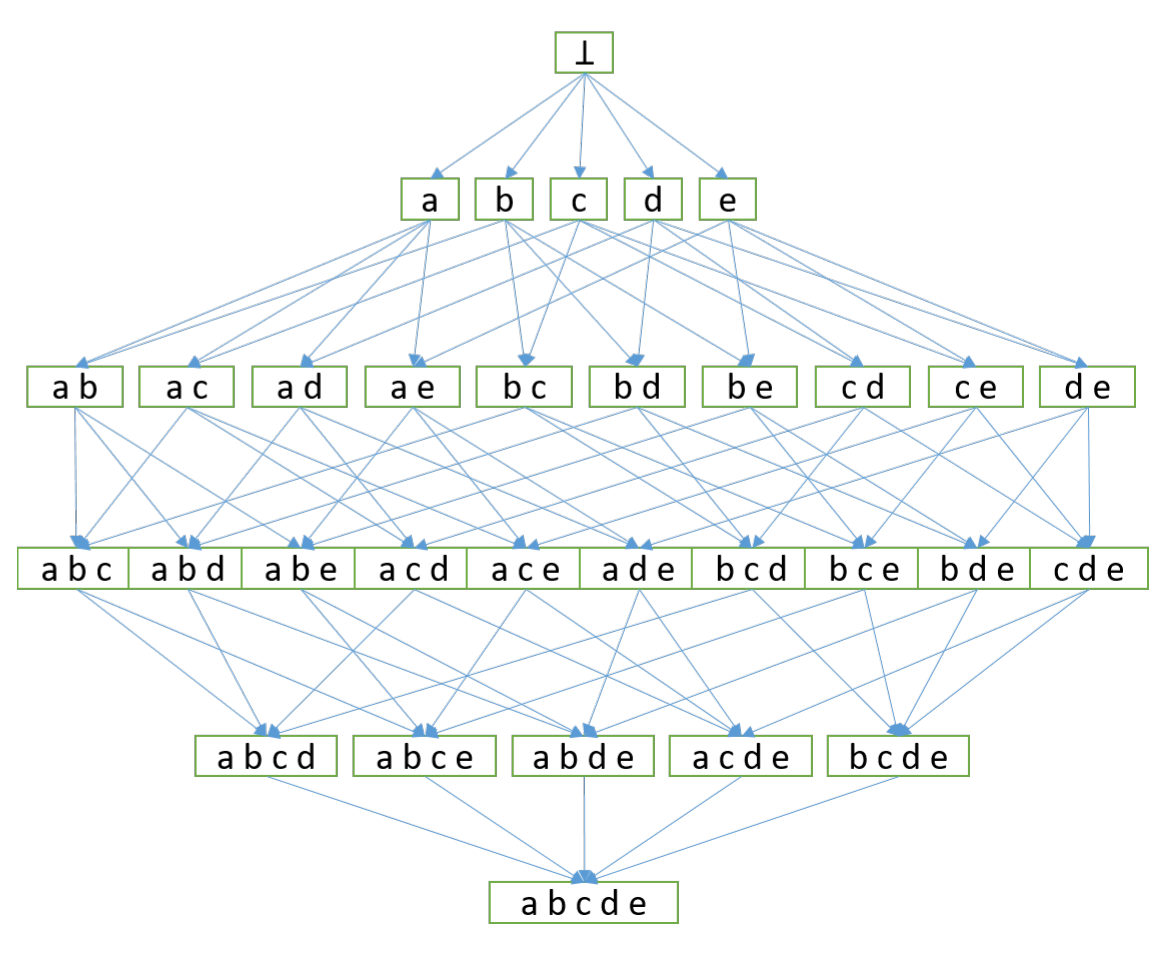
\includegraphics[width=5in]{lattices.eps}
\caption{Lattice representing the search space based on the items appearing in the example dataset $\mathcal{D}$}
\label{lattice}
\end{figure}


In this paper, we focus on closed itemsets.
Closed itemsets~\cite{ClosedPasquier1999} are a
particular and valuable subset of frequent itemsets, being
a concise but complete representation of the set of frequent itemsets. 
Precisely, an itemset $I$ is closed if none of its supersets (i.e. the set of itemsets which include $I$) has the same support count as $I$. For instance, in our running example, given a $minsup=2$, the itemset \textit{\{a,d\}} is a closed frequent itemset (support=3). The itemset \textit{\{a,c\}}, instead, is a frequent itemset (support=2), but it is not closed because of the presence of the itemset \textit{\{a,c,d\}} (support=2). 

A transactional dataset can also be represented in a vertical format, in which each
row represents an item $i$ and the list of tids of the transactions in which it appears,
also called $tidlist(\{i\})$.
For instance, the tidlist of the item \textit{a} in
the example dataset $\mathcal{D}$ is $\{1,2,4\}$.
Figure~\ref{back_TTexampledataset} reports the transposed representation of the
running example reported in Figure~\ref{back_horizontalexampledataset}. The main
advantage of the vertical format is the possibility to obtain the tidlist of
an itemset by intersecting the tidlists of the included items, without the
need of a full scan of the dataset.

\subsection{Centralized algorithms}
\label{centralized}
The search space exploration strategies of the distributed approaches are often inspired by the solutions adopted by the centralized approaches.
Hence, this section shortly introduces the main strategies of the centralized itemset mining algorithms. This introduction is useful to better understand the algorithmic choices behind the distributed algorithms.

The frequent itemset mining task is challenging in terms of execution time and memory consumption because the size of the search space is exponential with the number of items of the input dataset~\cite{goethals2003survey}.
Two main search space exploration strategies have been proposed: 
(i) level-wise or breadth-first exploration of the candidate itemsets in the lattice and 
(ii) depth-first exploration of the lattice.

The most popular representative of the breadth-first strategy is Apriori~\cite{apriori}. Starting from single items, it iteratively generates and counts the support of the candidate itemsets of size $k+1$ from the frequent itemsets of size $k$. At each iteration $k$, the supports of the candidate itemsets of length $k$ are counted by performing a new scan of the input dataset.
The search space is pruned by exploiting the downward-closure property, which guarantees that all the supersets of an infrequent itemset are infrequent
too. Specifically, the downward-closure property allows pruning the set of candidate itemsets of length $k+1$ by considering the 
frequent itemsets of length $k$.
The Apriori algorithm is significantly affected by the density of the dataset.
The higher the density of the dataset, the higher the number of frequent itemsets and hence the amount of candidate 
itemset stored in main memory. The problem becomes unfeasible when the number of candidate itemsets exceeds the size of the main memory.


More efficient and scalable solutions exploit the depth-first visit of the search space. 
FP-Growth~\cite{Han00}, which uses a prefix-tree-based main memory compressed representation of the input dataset, is the most popular depth-first based approach. 
The algorithm is based on a recursive visit of the tree-based representation of the dataset with a
``divide and conquer'' approach. In the first phase the support of each single item is
counted and only the frequent items are stored in the ``header table''. This information allows pruning the search space by avoiding the analysis of the itemsets extending infrequent items. Then, the FP-tree, that is a compact representation of the dataset, is built exploiting 
the header table and the input dataset. Specifically, each transaction is included in the FP-tree by adding or
extending a path on the tree, exploiting common prefixes. 
Once the FP-tree associated with the input dataset is built, FP-growth recursively splits the itemset mining problem 
by generating conditional FP-trees and visiting them.  Given an arbitrary prefix $p$, where $p$ is a set of items, the conditional FP-tree with respect to 
$p$, also called projected dataset with respect to $p$, is substantially the compact representation of the transactions containing  $p$. Each conditional FP-tree contains all the knowledge needed to extract all the frequent itemsets extending its prefix $p$. FP-growth decomposes the initial problem by generating one conditional FP-tree for each itemt $i$ and invoking
the itemset mining procedure on each of them, in a recursive depth-first fashion. 


FP-growth suits well dense datasets, because they can be effectively and compactly represented by means of the FP-tree data structure. Differently, with sparse datasets, the compressions benefits of the FP-tree are reduced because there will be a higher number of branches \cite{SurveyHan2007} (i.e., a large number of subproblems to generate and results to merge).

Another very popular depth-first approach is the Eclat algorithm~\cite{Zaki97newalgorithms}.
It performs the mining from a vertical
transposition of the dataset. In the vertical format, each transaction includes an item
and the transaction identifiers ($tid$) in which it appears ($tidlist$).
After the initial dataset
transposition, the search space is explored in a depth-first manner similar to
FP-growth. The algorithm is based on equivalence classes (groups of candidate itemsets
sharing a common prefix),  which allows smartly merging tidlists to select frequent itemsets. 
Prefix-based equivalence classes are mined independently, in a ``divide and conquer'' strategy, still
taking advantage of the downward closure property.
Eclat is relatively robust to dense datasets. It is less effective with sparse distributions, because the depth-first search strategy may require
generating and testing more (infrequent) candidate itemsets with respect to Apriori-like algorithms~\cite{vu2012mining}.



\section{Itemset mining parallelization strategies}
\label{parallelization}
Two main algorithmic approaches are proposed to address the parallel execution of the itemset mining algorithms by means of the MapReduce paradigm. 
They are significantly different because (i) they use different solutions to split the original problem in subproblems and (ii) make different assumptions about the data that can be stored in the main memory of each independent task. 

\begin{description}

\item[Data split approach.]  It splits the problem in ``similar'' subproblems, executing the same function on different data chunks. Specifically, each subproblem computes the local supports of all candidate itemsets on one chunk on the input dataset (i.e., each subproblem works on the complete search space but on a subset of the input data). Finally, the local results (i.e., the local supports of the candidate itemsets) emitted by each subproblem/task are merged to compute the global final result (global support of each itemset). The main assumptions of this approach are that (i) the problem can be split in ``similar' subproblems working on different chunks of the input data and (ii) the set of candidate itemsets is small enough that it can be stored in the main memory of each task.

\item[Search space split approach.]  It splits the problem by assigning to each subproblem the visit of a subset of the search space (i.e., each subproblem visits a part of the lattice). Specifically, this approach generates, from the input distributed dataset, a set of projected datasets, each one small enough to be stored in the main memory of a single task. Each projected dataset contains all the information that is needed to extract a subset of itemsets (i.e., each dataset contains all the information that is needed to explore a part of the lattice) without needing the contribution of the results of the other tasks. The final result is the union of the itemset subsets mined from each projected dataset.

\end{description}


\begin{figure}[!t]
\includegraphics[width=5in]{Approach1noniterativo.eps}
\caption{Itemset mining parallelization: Data split approach}
\label{approach1noniterativo}
\end{figure}

\begin{figure}[!t]
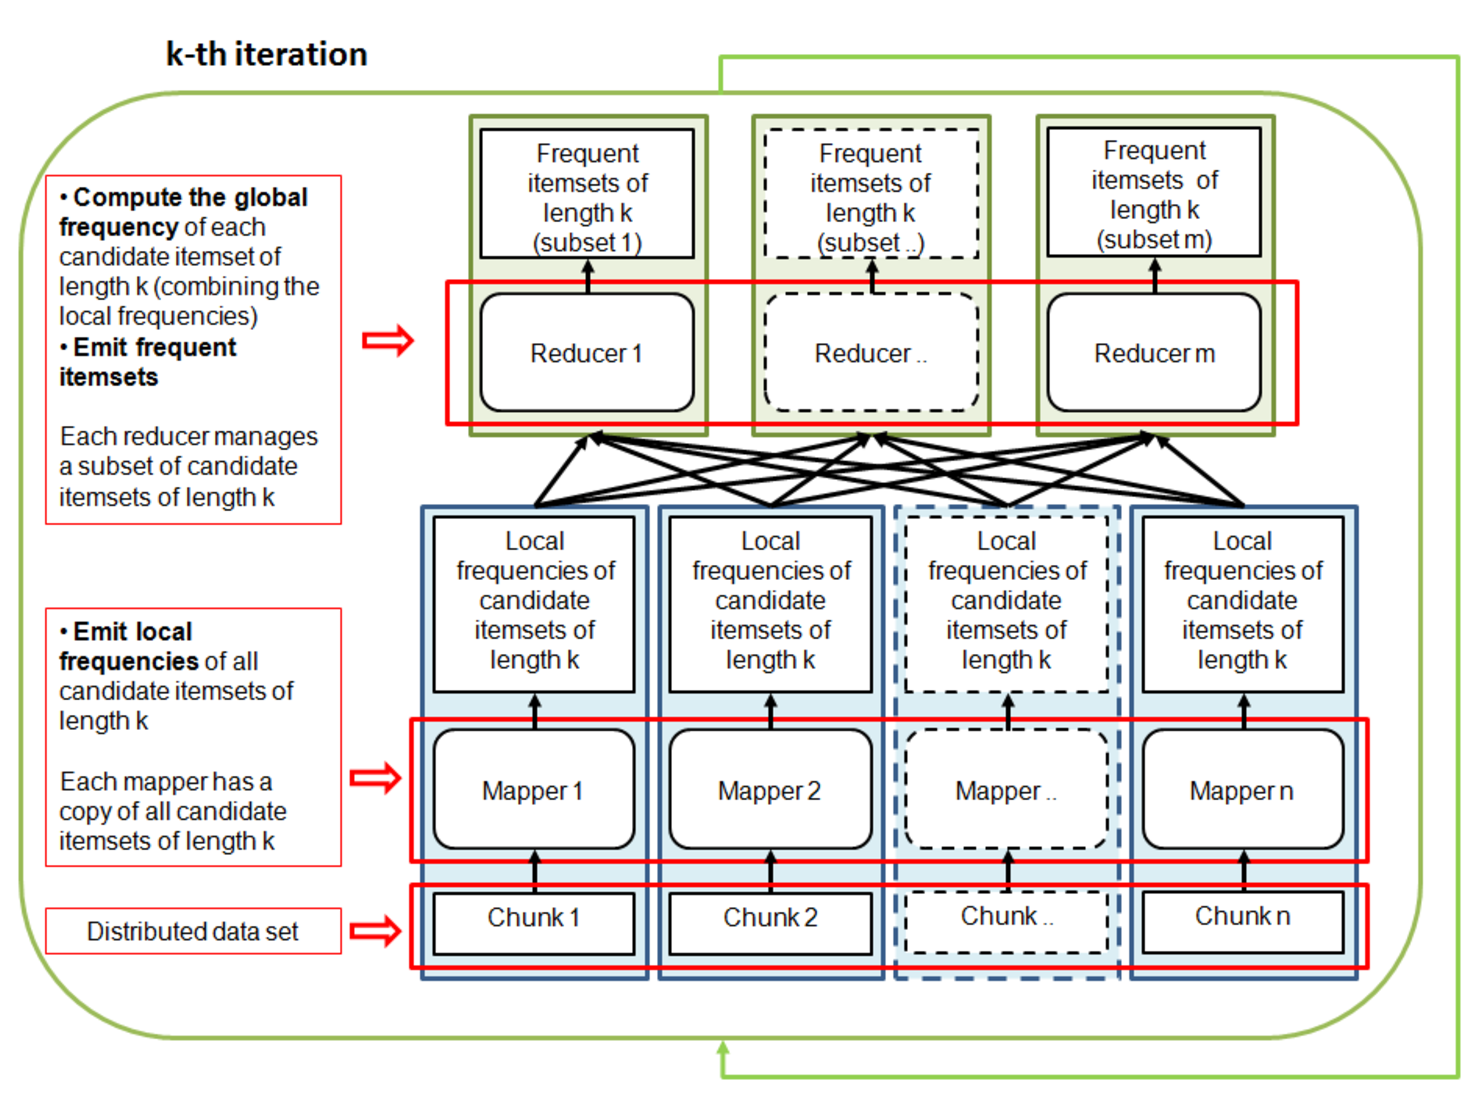
\includegraphics[width=5in]{Approach1.eps}
\caption{Itemset mining parallelization: Iterative Data split approach}
\label{approach1}
\end{figure}



\begin{figure}[!t]
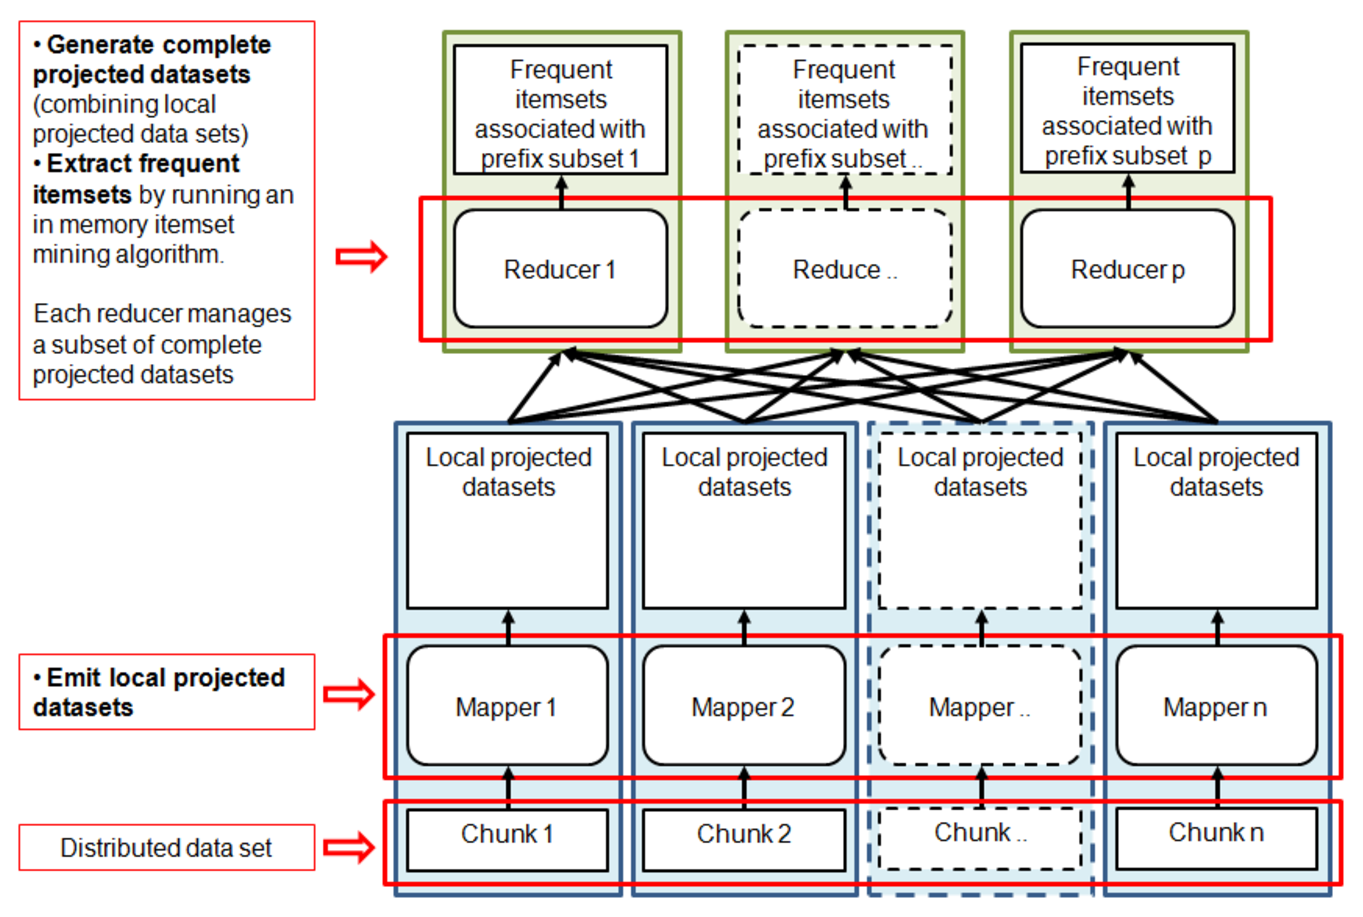
\includegraphics[width=5in]{Approach2.eps}
\caption{Itemset mining parallelization: Search space split approach}
\label{approach2}
\end{figure}


Figures~\ref{approach1noniterativo} and \ref{approach2} depict the first and the second parallelization strategies, respectively.  
In the data split approach (Figure~\ref{approach1noniterativo}), the map phase computes the local supports of the candidate itemsets in its data chunk  (i.e., each mapper runs a ``local itemset mining extraction'' on its data chunk). Then, the reduce phase merges the local supports of each candidate itemset to compute its global support. This solution requires each mapper to store a copy of the complete set of candidate itemsets (i.e., a copy of the lattice). 
This set must fit in the main memory of each mapper. Since the complete set of candidate itemsets is usually too large to be stored in the main memory of a single mapper, an iterative solution, inspired by the level-wise centralized itemset mining algorithms, is used. Figure~\ref{approach1} reports the iterative solution. 
At each iteration $k$ only the subset of candidates of length $k$ are considered and hence stored in the main memory of each mapper. This approach, thanks also to the exploitation of the apriori-principle to reduce the size of the candidate sets, allows obtaining subsets of candidate itemsets that can be loaded in the main memory of every mapper.

In the search space split approach (Figure~\ref{approach2}), the map phase generates a set of local projected datasets. Specifically each mapper generates a set of local projected datasets based on its data chunk. Each local projected dataset is the projection of the input chunk with respect to a prefix $p$.\footnote{Note that the projected datasets can overlap because the transactions associated with two distinct prefixes $p_1$ and $p_2$ can be overlapped.} Then, the reduce phase merges the local projected datasets to generate the complete projected datasets. Each complete projected dataset is provided as input to a standard centralized itemset mining algorithm running in the main memory of the reducer and the set of frequent itemsets associated to it are mined.
Each reducer is in charge of analyzing a subset of complete projected datasets by running the itemset mining phase on one complete projected dataset at a time.   
Hence, the main assumption, in this approach, is that each complete projected dataset must fit in the main memory of a single reducer. 

Table~\ref{tab:assumptions} summarizes the main characteristics of the two parallelization approaches with respect to the following criteria: 
type of split of the problem, 
usage of main memory, 
communication costs, 
load balancing, 
and maximum parallelization (i.e. maximum number of mappers and reducers).
%These are important issues to be addressed by distributed algorithms to increase their efficiency. 

%The communication cost is the amount of data sent on the network across the nodes of the cluster. The network can quickly  become the bottleneck 
%if large amount of data are sent on it. Hence, appropriate solutions must be adopted to limit it. 
%Load balancing is another important issue. It aims at assigning similar subproblems, characterized by similar execution times, to the nodes of the cluster to maximize the use of the available resources. A well-balanced application allows exploiting, simultaneously, all the available resources, whereas a non-well balanced applications is characterized by busy nodes (the ones associated with the longest tasks) and idle ones (the ones associated with the shortest tasks).

%For completeness, Table~\ref{tab:assumptions} reports both versions of Approach~1. However, the actual implementations are not based on the non-iterative version of Approach~1 because the complete set of itemsets (i.e., the complete lattice) is too large to be stored in main memory.


%\begin{table}[]
%\scriptsize
%\centering
%\caption{Comparison of the parallelization approaches.}\label{tab:assumptions}
%\begin{tabular}{|p{1.5cm}|p{3cm}|p{3cm}|p{3cm}|p{2cm}|}
%\hline {\bf Name} & {\bf Assumption} & {\bf Communication costs} & {\bf Load balancing} & {\bf Number of reads of the distributed dataset} \\
%\hline
%\hline Approach~1 (Figure~\ref{approach1noniterativo})& The complete set of candidate itemsets (i.e., the complete lattice) can be stored in the main memory of a single task. & Number of candidate itemsets $\times$ number of mappers. & Load balancing is achieved by associating the same number of itemsets to each reducer. & 1 \\
%
%\hline Approach~1 - Iterative version (Figure~\ref{approach1}) & Each candidate set of itemsets of length $k$ can be stored in the main memory of a single task. & Number of candidate itemsets $\times$ number of mappers $\times$ number of iterations. & Load balancing is achieved by associating the same number of itemsets to each reducer. & number of iterations (= size of the longest frequent itemset)\\
%\hline Approach~2 (Figure~\ref{approach2})& Each global projected dataset can be stored in the main memory of a single task. & Sum of the sizes of the local projected datasets. & Load balancing is not addressed. The tasks could be significantly unbalanced depending on the difference among the projected datasets and the related mining processes. & 1 \\
%\hline
%\end{tabular}
%\end{table}



\begin{table}[]
\scriptsize
\centering
\caption{Comparison of the parallelization approaches.}\label{tab:assumptions}
\begin{tabular}{|p{2.5cm}|p{5cm}|p{5cm}|}

\hline {\bf Criterion} & {\bf Iterative data split approach (Figure~\ref{approach1})} & {\bf Search space split approach (Figure~\ref{approach2})} \\
\hline
%\hline Type of split/Split of the search space &  All subproblems/mapper tasks analyze all the candidate itemsets of length $k$, but each one works on a different chunk of data. The final result is given by the merge of the local results.  &  Each subproblem analyzes a different subset of itemsets/a different part of the search space. The final result is the union of the local results. \\
\hline Type of split/Split of the search space &  Each subproblem analyzes a different subset of the input data and computes the local supports of 
all the candidate itemsets of length $k$ on its chunks of data. The final result is given by the merge of the local results.  &  Each subproblem analyzes a different subset of itemsets/a different part of the search space. The final result is the union of the local results. \\
\hline Usage of main memory &  The candidate set of length $k$ is stored in the main memory of a single task. & The complete projected dataset is stored in the main memory of a single task. \\
\hline Communication cost &  Number of candidate itemsets $\times$ number of mappers $\times$ number of iterations. & Sum of the sizes of the local projected datasets. \\
\hline Load balancing &  Load balancing is achieved by associating the same number of itemsets to each reducer. & The tasks could be significantly unbalanced depending on the characteristics of the projected datasets assigned to each node.\\
\hline Maximum number of mappers & Number of chunks  & Number of chunks  \\
\hline Maximum number of reducers & Number of candidate itemsets  & Number of items \\
\hline
\end{tabular}
\end{table}

%\begin{table}[]
%\scriptsize
%\centering
%\caption{Comparison of the parallelization approaches.}\label{tab:assumptions}
%\begin{tabular}{|p{2cm}|p{3.4cm}|p{3.4cm}|p{3.4cm}|}
%
%\hline {\bf Criterion} & {\bf Approach~1 (Figure~\ref{approach1noniterativo})} & {\bf Approach~1 - Iterative version (Figure~\ref{approach1})} & {\bf Approach~2 (Figure~\ref{approach2})} \\
%\hline
%\hline Type of split/Split of the search space & All subproblems/mapper tasks analyze all the candidate itemsets (i.e., work on the whole search space), but each one work on a different chunk of data. The final result is given by the merge of the local results.  & All subproblems/mapper tasks analyze all the candidate itemsets of length $k$, but each one work on a different chunk of data. The final result is given by the merge of the local results.  &  Each subproblem analyzes a different subset of itemsets/a different part of the search space. The final result if the union of the local results. \\
%\hline Use of the main memory & The complete set of candidate itemsets (i.e., the complete lattice) can be stored in the main memory of a single task.  &  Each candidate set of itemsets of length $k$ can be stored in the main memory of a single task. & Each global projected dataset can be stored in the main memory of a single task. \\
%\hline Communication costs & Number of candidate itemsets $\times$ number of mappers. &  Number of candidate itemsets $\times$ number of mappers $\times$ number of iterations. & Sum of the sizes of the local projected datasets. \\
%\hline Load balancing & Load balancing is achieved by associating the same number of itemsets to each reducer. &  Load balancing is achieved by associating the same number of itemsets to each reducer. & The tasks could be significantly unbalanced depending on the characteristics of the projected datasets assigned to each node and the related mining processes. Load balancing can not be easily achieved.\\
%%\hline Number of reads of the distributed dataset & 1 & Number of iterations (= size of the longest frequent itemset)  & 1 \\
%\hline Maximum number of mappers & Number of chunks & Number of chunks  & Number of chunks  \\
%\hline Maximum number of reducers & Number of candidate itemsets & Number of candidate itemsets  & Number of items \\
%\hline
%\end{tabular}
%\end{table}


\noindent{\bfseries Type of split/Split of the search space}. 
The main difference between the two parallelization approaches is the strategy adopted to split the problem in subproblems. This choice has a significant impact on the other criteria.

\noindent{\bfseries Usage of main memory}. 
The different usage of the main memory of the tasks impact on the reliability of the two approaches. The data split approach assumes that the candidate itemsets of length k can be stored in the main memory of each mapper. Hence, it is not able to scale on dense datasets
characterized by large candidate sets. Differently, the search space split approach assumes that each complete projected dataset can be stored in the main memory of a single task. Hence, this approach runs out of memory when large complete projected datasets are generated.  

\noindent{\bfseries Communication costs}. In a parallel MapReduce algorithm, communication costs are important, because the network can easily become the bottleneck if large amounts of data are sent on it.
The communication costs are mainly related to the outputs of the mappers which are sent to the reducers on the network. 
For the data split approach the data that is sent on the network is linear with respect 
to the number of candidate itemsets, the number of mappers, and the number of iterations.
Differently, for the search space approach, the amount of data emitted by the mappers is equal to the size of the projected datasets. 
%Since the projected datasets are overlapped the result is that the data sent across the network is potentially larger than the initial dataset\footnote{Usually, the size of the data sent on the network is not large as the initial dataset because compact trees are used to represent the projected datasets.}. 


\noindent{\bfseries Load balancing}. 
The different split of the problem in subproblems significantly impacts on load balancing. For the data split approach, the execution time of each mapper 
is linear with respect to the number of input transactions and the execution time of each reducer is linear with respect to the number of assigned itemsets.
Hence, the data split approach can easily achieve a good load balancing by assigning the same number of data chunks to each mapper and the same number of candidate itemsets to each reducer. 
Differently, the search space split approach is potentially unbalanced. In fact, each subproblem is associated with a different subset of the lattice, related to a specific projected dataset and prefix, and, depending on the data distribution, the complexity of the subproblems can significantly vary. 
A smart assignment of a set of subproblems to each node would mitigate the unbalance. However, the complexity of the subproblems is hardly inferable during the initial assignment phase.

\noindent{\bfseries Maximum number of mappers and reducers}. 
The two approaches are significantly different in terms of ``maximum parallelization degree'', at least in terms of number of maximum exploitable reducers. 
The maximum parallelization of the map phase is equal to the number of data chunks for both approaches.
% (i.e., maximum number of mappers = number of data chunks). 
Differently, the maximum parallelization of the reduce phase is equal to the number of candidate itemsets for the data split approach, because potentially each reducer could compute the global frequency of a single itemset, whereas it is equal to the number of global projected datasets for the second approach, which can be at most equal to the number of items. 
Since the number of candidate itemsets is greater than the number of items, the data split approach can potentially reach a higher degree of parallelization with respect to the search space split approach. 


%The communication costs are related to the outputs of the mappers. Since each mapper of the first approach emits one local support for each candidate itemset, the data that is sent on the network is linear with respect to the number of candidate itemsets and the number of mappers.
%Differently, for the second approach, the amount of data emitted by the mappers is equal to the size of the projected datasets. Since the projected datasets are overlapped the result is that the data sent across the network is potentially larger than the initial dataset\footnote{Usually, the size of the data sent on the network is not large as the initial dataset because compact trees are used to represent the projected datasets.}. 
%
%The different split of the problem in subproblems impacts also on load balancing. The first approach can easily achieve load balancing because all mappers perform the same operation and also all reducers perform the same operation. The only difference is given by the input data chunks and input candidate itemsets. By assigning the same number of data chunks to each mapper and the same number of candidate itemsets to each reducer, the result is that all mapper tasks are characterized by a similar execution time and also all reducers are characterized by a similar execution time. This means that the overall application is well-balanced. 
%Differently, the second approach is potentially unbalanced. In fact, each subproblem is associated with a different subspace of the search space, related to a specific projected dataset and prefix, and, depending on the data distribution, the complexity of the subproblems can significantly vary. A smart assignment of a set of subproblems to each node would mitigate the unbalance. However, the complexity of the subproblems is hardly inferable during the initial assignment phase.
%
%
%The two approaches are also different in terms of ``maximum parallelization degree'', at least in terms of number of maximum exploitable reducers. 
%The maximum parallelization of the map phase is equal to the number of data chunks for both approaches (i.e., maximum number of mappers = number of data chunks). Differently, the maximum parallelization of the reduce phase is equal to the number of candidate itemsets for the first approach, because potentially each reducer could compute the final frequency of a single itemset, whereas it is equal to the number of global projected datasets for the second approach, which can be at most 
%equal to the number of items. 
%Since the number of candidate itemsets is greater than the number of items, the first approach can reach a higher degree of parallelization with respect to the second approach. However, pay attention that a higher number of reducers corresponds also to a higher overhead related to the instantiation of the reducers. 

The two parallelization approaches are used to design efficient parallel implementations of well-known centralized itemset mining algorithms.  Specifically, the data split approach is used to implement the parallel versions of level-wise algorithms (like Apriori~\cite{apriori}), whereas the search space split approach is used to implement parallel versions of depth-first recursive approaches (like FP-growth~\cite{Han00} and Eclat~\cite{Zaki97newalgorithms}). 
%The map phase of the second approach can be seen as the first step of the recursion, that is used to generate the datasets projected with respect to prefixes composed of single items. Then, the reduce phase runs, in main memory, one instance of the mining algorithm for each projected dataset.




%{\bfseries Paolo: Capire cosa tenere della parte dopo che era la vecchia versione di questa sezione.}
%
%\textbf{Fabio: la metterei dopo l'intro degli algoritmi} In this section, we describe the main algorithmic solutions that have been exploited to address the
%parallelization of the itemset mining problem in the big data distributed environments (e.g., Hadoop and Spark).
%Many considerations are general and independent of the big data nature of the input data, whereas some other considerations and 
%algorithmic/design choices are driven by the big data characteristics of the input data (e.g., design of algorithms that exploit data locality).
%
%The parallelization and distributed execution of a generic algorithm, in the big data environment, is usually based on the split of the main task 
%in subtasks, each one working in isolation (shared-nothing) on one chunk of the data. However, this approach is not always possible and hence some algorithms 
%share small portions of data among the parallel tasks.
%
%The Hadoop-based algorithms usually parallelize the addressed problems by splitting the input datasets in independent data chucks. 
%Each chuck of the input data is assigned to a subtask that analyses the chunk of data in isolation (i.e., without needing the information 
%available in the other chunks). This is the map phase of the MapReduce programming paradigm. The outputs generated by the subtasks
%are then merged to obtain the final output (i.e., the output of the algorithm applied on the whole data). This second step is the reduce phase.
%The main assumptions of this solution are that (i) the input dataset is big (hence it cannot be sent on the network), whereas the outputs of 
%the subtasks are small and can be sent on the network and shared across the nodes of the cluster and (ii) the initial problem 
%can be split in subproblems each one working on one portion of the data and the portions are not overlapped.
%
%
%The algorithms that address the frequent itemset mining (FIM) \textbf{Fabio: FIM secondo me è piu' usato di FIMI} problem in the distributed environment can be grouped in two classes, based on how they split the problem: 
%\begin{enumerate}
%\item Data split approaches. These approaches parallelize the FIM problem by using the standard Hadoop-based approach, i.e., by splitting the data and assigning to each subtask one chunk.
%
%\item Search space split approaches. These approaches parallelize the FIM problem by splitting the search space, i.e., by assigning to each
% subtask the visit of a part of the  search space, even if this implies partial overlapping between the portions of data used by each subtask and 
% sending potentially large portions of the data on the network. 
%\end{enumerate}
%
%The algorithms of the first class exploit data locality, which is usually the most important point for the efficiency and scalability of 
%the MapReduce-based algorithms. However, when dealing with the itemset mining problem, 
%these solutions need to share common knowledge among the main memory 
%of the subtasks and the problem explodes when the amount of shared knowledge is larger than the main memory of each single task. Moreover, in this environment, they
%are iterative solutions that need to read multiple times the input dataset and this can be a problem when dealing with big data (the optimal solution
%should read only once the input dataset).
%
%%The algorithms belonging to the second class adopt a strategy that is not the ``standard'' one when the MapReduce programming paradigm is used,
%%because they are focused on the split of the search space and not on the split, without overlapping, of the input dataset.
%The algorithms belonging to the second class adopt a different strategy. While the MapReduce ``standard'' behavior assumes to split the input data in chunks and use them for the computation, in this case the search space is split in subproblems. Unfortunately, the result of this type of partitioning is that the input and the data structures of the obtained subproblems overlap. \textbf{Fabio: Dobbiamo introdurre meglio questo search space visto che ne parliamo cosi tanto}
%However,
%often these approaches are more efficient then the ones of the first class, especially when long patterns are mined (the longer the mined 
%patterns, the greater the number of times the input dataset is read when using the algorithms of the first class). 
%
%%Another important difference between the second class of algorithms and the first one is that the second class of algorithms 
%%aims at splitting the initial problem in subproblems that can be executed in ``main memory'', i.e., subproblems such that
%%the data of each subproblem can be stored in the main memory of one single task and a ``centralized' version of the mining problem can be 
%%executed in each task.
%
%Another important difference between the second class of algorithms and the first one is that such subproblems can be executed in  ``main memory''. In these cases, each subproblem is independent and is computed with a routine often inherited from a non-distributed frequent itemset mining algorithm.
%
%
%Among the 
%%available parallel big data itemset mining algorithms,
%considered algorithms
% YAFIM belongs to the first class while the two FP-Growth-based algorithms (i.e. Mahout and MLlib PFP) and DistEclat belong to the second class.
%BigFIM adopts a mixed approach (the first phase is related to the first class of algorithms and the second phase to the second class).  
%
%
%Another classification of the available algorithms is based on how they visit the search space. By using this criterion the algorithms can be classified in 
%two classes:
%\begin{enumerate}
%\item Breadth first approaches, also called level-wise approaches. These are iterative approaches that, at each iteration, visit a level of the 
%lattice of candidate itemsets/of the search space (i.e., at iteration $k$ mines the frequent itemset of length $k$).
%
%\item Depth first approaches. These approaches visit the search space by using a is a depth first strategy. 
%\end{enumerate}
%
%YAFIM belongs to the breadth first class, PFP and DistEclat belong to the Depth first approaches, while BigFIM uses a mixed approach (bread first for
%the mining of the itemset of length less than $k$ and depth first for the mining of the longer itemsets).
%\textbf{Fabio: non so se lo presenterei come due classificazione e poi associarle o direttamente come una sola perchè secondo me questi aspetti sono legatissimi}
%The groups of algorithms identified by the two classification criteria are the same because the breadth first approaches, for the itemset mining problem,
%fit well a parallelization based on the split of the input data, whereas the depth first approaches fix better a parallelization solution based on the 
%the split of the search space.
%
%


%\section{Evaluation criteria}
%\label{criteria}
%The main target of this review is to build a structured comparison among the
most popular frequent itemset miners in distributed environments.
For this reason, we define a set of criteria
which can be divided into two groups, summarized in Table~\ref{tab:evalcriteria}.

The first group, named \textit{algorithmic strategy}, is strictly related to the centralized frequent itemset algorithms from which the distributed implementations are derived. 
Itemset discovery algorithms, proposed for the distributed frameworks, are not designed from scratches to be distributed or parallelized. Often, the main contribution introduced in the domain is the implementation of well-known techniques to distributed environment. Thus, the main research efforts are moved from the algorithm design to the following points:

\begin{itemize}

\item The distribution
of tools or algorithms that were not designed to be distributed (i.e. splitting
the computation load into more than one node). In addition, data mining
algorithms are often characterized by the need of a full knowledge of the
problem or data. In other words, data mining problems are often not
"embarassingly parallelizable". This issue makes the distribution very
challenging.

\item A well-engineered transposition to distributed frameworks,
exploiting the advantages and features of the platforms. For instance,
exploiting data locality in MapReduce-based implementations provides a
fundamental performance boost. Another example is the optimized ``shuffle \&
sort'' phase, which represents the unique phase in which data can be sent to other
nodes. Transposing an algorithm into MapReduce can be very challenging because
of its limitations, whereas one of the advantages of Apache Spark over Hadoop
is a  greater flexibility.

\end{itemize}

Hence, the underlying centralized algorithms
are very important to describe and evaluate the scalable approaches. Some of
their features are directly inherited by the distributed algorithms.

Specifically, we have selected two criteria, as reported in Table~\ref{tab:evalcriteria}, directly inherited from the underlying centralized approaches, named the candidate itemset generation phase~\cite{goethals2003survey}. 

\begin{enumerate}

\item \textit{The search space exploration strategy} allows decomposing the mining task into a set of smaller tasks to dramatically reduce the computation cost. Different strategies have been exploited in performing the itemset mining as divide-and-conquer, depth-first methods or level-wise, breadth-first generation methods.  Each strategy can yield good performance when dealing with a given data distribution. 

\item \textit{The data distribution}. Each collection of data is characterized by a given distribution varying based on the number of transactions, average transaction length (average number of objects in a given transaction, and the cardinality of different objects. Datasets are
usually characterized by an inherent sparseness when a large number of transactions appear with a limited/shorter average transaction length, and a large variety of different objects/items. The sparseness in data distribution
increases with data volume and cardinality of different objects.
Although a formal and universal definition of data distribution is not yet available in the domain of itemset mining, it is well-known that a given algorithm is typically suited for a given data distribution, thus its performance are the best for some datasets or under some input parameter values and the worst in other cases. In general, the execution cost of a given algorithm tends to increase when dealing with dense datasets or large data volume with an inherent sparseness but with low support thresholds. In these both conditions, a large number of itemsets have to be generated. \end{enumerate}

The performance of the algorithms that adopt a level-wise or breadth-first exploration  (i.e. algorithms that generate candidate itemsets of length $k$ from itemsets of length $k-1$) is negatively affected by a large average transaction width, because more candidate itemsets must be examined~\cite{KumarBook}. Since average transaction width is strongly related to the input data distribution, there exists a relationship between the exploration strategy and the input dataset distribution. For example, Apriori-based algorithms~\cite{Agr94}, detailed in Subsection~\ref{bigfim}, with their breadth-first exploration approach, better fit datasets characterized by
sparse distributions, i.e. low correlation among patterns and high item cardinality.



The second set of evaluation criteria is related to the distributed nature of
the processing. They are often undervalued in the data mining context but
represent critical
issues~\cite{afrati2012designing},~\cite{leskovec2014mining}.

\begin{enumerate}

\item Communication costs: this issue is often underestimated in distributed
algorithms, but they represent the most likely bottleneck of a distributed
system~\cite{sarma2013upper}. In the design phase, most of the researchers focus
only on the computational costs and the need to split them among the nodes. The
result is that a great amount of data is sent through the network, making
communication costs much higher than computational costs.
% In addition, as already
% mentioned, many data minings algorithms were designed for centralized systems,
% ignoring these kinds of factors. However, the data locality paradigm is one of
% the reason of the effectiveness of distributed platforms such as Hadoop or
% Spark. Thus, the implementations in this review will be evaluated also through
% the care or attention devoted to this aspect.

\item Load balancing: since one of the main goals of a distributed
approach is to decrease the overall execution time, load balancing is required
to efficiently reach such objective. An unbalanced load
undermines the advantages of a parallel environment: the overall execution time
is that of the slowest, most loaded node. In a fully unbalanced environment, the
worst case scenario leads to no benefits from parallelization while still
incurring all the overheads of coordinating a rather complex distributed system.

\end{enumerate}

A review of the evaluation criteria is presented in
Table~\ref{tab:example1}. After a qualitative review of the algorithms in
Section~\ref{algorithms}, in Section~\ref{experimental} an experimental
performance evaluation is provided.

%
%\begin{table*}[]
%\scriptsize
%\centering
%\caption{Overview of valution criteria. \label{tab:evalcriteria}}
%\begin{tabular}{| c|c|c|c|}
%\hline {\bf Class Name} & {\bf Property of} & {\bf Criterion name} & {\bf Domain} \\ \hline
%\hline Algorithmic & Centralized  & The search space & $\{$Depth First,  \\
%strategy & approaches & exploration strategy & Breadth First $\}$  \\
%\hline 
%& & Data distribution & $\{$dense, sparse$\}$ \\  \hline
%
%\hline 
%Distributed & Distributed  & Communication & $\{$Yes, No$\}$ \\
%processing & approaches & cost handling & \\
%\hline 
%& & Load balancing & $\{$Yes, No$\}$ \\
%& & handling &  \\
%\hline 
%\end{tabular}
%\end{table*}


\begin{table*}[]
\scriptsize
\centering
\caption{Overview of evaluation criteria. \label{tab:evalcriteria}}
\begin{tabular}{| c|c|c|c|}
\hline \textbf{Class Name}                                                               & \textbf{Property of}                                                              & \textbf{Criterion name}                                                                           & \textbf{Domain}                                                                             \\ \hline \hline
\multirow{3}{*}{\begin{tabular}[c]{@{}c@{}}Algorithmic \\ strategy\end{tabular}}  & \multirow{3}{*}{\begin{tabular}[c]{@{}c@{}}Centralized\\ approaches\end{tabular}} & \multirow{2}{*}{\begin{tabular}[c]{@{}c@{}}The search space \\ exploration strategy\end{tabular}} & \multirow{2}{*}{\begin{tabular}[c]{@{}c@{}}\{ Depth First,\\  Breadth First\}\end{tabular}} \\
                                                                                  &                                                                                   &                                                                                                   &                                                                                             \\ \cline{3-4} 
                                                                                  &                                                                                   & Data distribution                                                                                 & \{ dense, sparse \}                                                                         \\ \hline
\multirow{4}{*}{\begin{tabular}[c]{@{}c@{}}Distributed\\ processing\end{tabular}} & \multirow{4}{*}{\begin{tabular}[c]{@{}c@{}}Distributed\\ approaches\end{tabular}} & \multirow{2}{*}{\begin{tabular}[c]{@{}c@{}}Communication\\ cost handling\end{tabular}}            & \multirow{2}{*}{\{ Yes, No \}}                                                               \\
                                                                                  &                                                                                   &                                                                                                   &                                                                                             \\ \cline{3-4} 
                                                                                  &                                                                                   & \multirow{2}{*}{\begin{tabular}[c]{@{}c@{}}Load balancing\\ handling\end{tabular}}                & \multirow{2}{*}{\{ Yes, No \}}                                                               \\
                                                                                  &                                                                                   &                                                                                                   &                                                                                             \\ \hline
\end{tabular}
\end{table*}



\section{Distributed itemset mining algorithms}
\label{algorithms}
%\begin{table}[]
%\scriptsize
%\centering
%\caption{Classification.}\label{tab:example1}
%\begin{tabular}{|c|c|c|c|c|c|}
%\hline 					& \multicolumn{5}{|c|}{\bf Distributed Algorithm/Implementation} \\
%\cline{2-6} {\bf Criterion} & {\bf Mahout PFP} & {\bf MLlib PFP} & {\bf Dist-Eclat} & {\bf BigFIM} & {\bf YAFIM} \\
%\hline
%\hline
%Search space & Depth First & Depth First & Depth First & Breadth First & Breadth First \\
%exploration  & & & & and  & \\
%strategy     & & & & Depth First & \\
%\hline
%Data  			  & Dense & Dense & Dense & Sparse & Sparse \\
%distribution	  & & & & and  &  \\
%				  & & & & dense  &  \\
%\hline
%Parallelization  & Search space & Search space & Search space & Data split & Data \\
%strategy         &  		& & & and  & split \\
%          &  		& & & Search space &  \\
%          &  		& & & split &  \\
%\hline
%Communication  & Yes & Yes & Yes & Yes  &  Yes  \\
%cost           & & & (trade-off & (trade-off &  \\
%handling       & & & with load & with load &  \\
%		       & & & balancing) & balancing) &  \\
%\hline
%Load balancing & No & No & Yes & Yes & No \\
%handling  & & & & &  \\
%\hline
%Framework  & Hadoop & Spark & Hadoop & Hadoop &  Spark  \\
%\hline
%Underlying centralized  & FP-Growth & FP-Growth & Eclat & Apiori &  Apriori \\
%algorithm  & & &  & and Eclat &  \\
%\hline
%\end{tabular}
%\end{table}



This section describes the algorithms, and available implementations, representing the state-of-the-art
solutions in the parallel frequent itemset mining context. We considered the following algorithms: YAFIM~\cite{YAFIM},
PFP~\cite{pfpgrowth},
BigFIM~\cite{bigfim}, and DistEclat~\cite{bigfim}.
The only algorithm which is lacking a publicly available implementation is YAFIM.
Among the considered algorithms, YAFIM belongs to the ones based on the data split approach, 
while PFP and DistEclat are based on the search space split approach. Finally, BigFIM mixes the two strategies, aiming at exploiting the pros of them.
For PFP we selected two popular implementations: Mahout PFP and MLlib PFP, which are based on Hadoop and Spark, respectively.  
The description of the four selected algorithms and their implementations are reported in the following subsections.

%\begin{table*}[]
%\scriptsize
%\centering
%\caption{Comparison summary. \textbf{Fabio: Aggiungere Parallelization!}\label{tab:example1}}
%\begin{tabular}{| c|c|c|c|c|c|c|}
%\hline {\bf Name} & {\bf Framework} & {\bf Underlying} & {\bf Data} & {\bf Search} & {\bf Comm.} & {\bf Load  }\\
%& & {\bf centralized} & {\bf distrib.} & {\bf strategy} & {\bf cost handling} & {\bf balance}\\
%& & {\bf algorithm} &&& & {\bf handling}\\
%\hline
%\hline Mahout PFP & Hadoop & FP-Growth & Dense & Depth First & Yes & No\\
%\hline MLlib PFP & Spark & FP-Growth & Dense & Depth First & Yes & No\\
%\hline Dist-Eclat & Hadoop & Eclat & Dense & Depth First & Yes & Yes \\
% &  &  &  &  & (trade-off with &  \\
% &  &  &  &  & load balancing) &  \\
%\hline BigFIM & Hadoop & Apriori and & Dense and  & Breadth First & Yes & Yes\\
%  &  & Eclat & sparse &  and &  (trade-off  with & \\
%   &  &  &  &Depth First  & load balancing) &  \\
%\hline YAFIM & Spark & Apriori & Sparse & Breadth First & Yes & No\\
%\hline
%\end{tabular}
%\end{table*}


%\begin{table}[]
%\scriptsize
%\centering
%\caption{Comparison summary.}\label{tab:example1}
%\begin{tabular}{|c|c|c|c|c|c|c|}
%\hline {\bf Name} & {\bf Framework} & {\bf Underlying} & {\bf Data} & {\bf Search} & {\bf Comm.} & {\bf Load  }\\
%& & {\bf centralized} & {\bf distrib.} & {\bf strategy} & {\bf cost} & {\bf balance}\\
%& & {\bf algorithm} &&& {\bf handling}& {\bf handling}\\
%\hline
%\hline Mahout PFP & Hadoop & FP-Growth & Dense & Depth First & Yes & No\\
%\hline MLlib PFP & Spark & FP-Growth & Dense & Depth First & Yes & No\\
%\hline Dist-Eclat & Hadoop & Eclat & Dense & Depth First & Yes & Yes \\
% &  &  &  &  & (trade-off with &  \\
% &  &  &  &  & load balancing) &  \\
%\hline BigFIM & Hadoop & Apriori and & Dense and  & Breadth First & Yes & Yes\\
%  &  & Eclat & sparse &  and &  (trade-off  with & \\
%   &  &  &  &Depth First  & load balancing) &  \\
%\hline YAFIM & Spark & Apriori & Sparse & Breadth First & Yes & No\\
%\hline
%\end{tabular}
%\end{table}


\subsection{YAFIM}
{\bf YAFIM}~\cite{YAFIM} is an Apriori distributed implementation developed in Spark.
%Apriori works well with sparse datasets and it is characterized by a different behavior with respect to Eclat and FP-growth: 
The iterative nature of the algorithm has always represented a challenge for its application in MapReduce-based Big Data
frameworks. The reasons are the overhead caused by the launch of new MapReduce
jobs and the requirement to read the input dataset from disk at each
iteration. YAFIM exploits Spark RDDs to cope with these issues. Precisely, it
assumes that all the dataset can be loaded into an RDD to speed up the
counting operations. Hence, after the first phase in which all the transactions
are loaded in an RDD, the algorithm starts the iterative Apriori algorithm organizing
the candidates in a hash tree to speed up the search.
Being strongly Apriori-based, it inherits the breadth-first strategy to explore and partition
the search space and the preference towards sparse data distributions.
YAFIM exploits the Spark ``broadcast variables abstraction'' feature, which allows
programmers to send subsets of shared data to each slave only once,
rather than with every job that uses those subset of data. This
implementation mitigates communication costs (reducing the inter job
communication), while load balancing is not addressed.

\subsection{Parallel FP-growth (PFP)}
\label{FP-Growth}
%FP-growth~\cite{Han00}, as mentioned, is among the most popular approaches for frequent pattern mining.
%It is based on a transposition of the
%whole dataset into a main memory compressed representation of the database
%called FP-tree. The algorithm is based on a recursive visit of the tree with a
%“divide and conquer”, partitioning-based approach. In the first phase the support of the items is
%counted to build the ``header table''. Then, the FP-tree is built exploiting the
%header table and the input dataset: each transaction is included adding or
%extending a path on the tree, exploiting common prefixes. Finally, for each
%item, it extracts the frequent itemsets from the item’s conditional FP-tree, in
%a recursive, depth first fashion. For the nature of the FP-tree, it is very robust to dense datasets. With a sparse dataset, the
%benefits of the FP-tree transposition would be reduced because there would be a
%higher number of branches and paths \cite{KumarBook} (i.e. a large number of
%subproblems to generate and results to merge).
%It is based on an FP-tree transposition of the transaction dataset and a
%recursive ``divide and conquer'' visit of the FP-tree. FP-Growth algorithm,
%instead, exploits a a main memory compressed representation of the database
%called FP-tree. The algorithm is based on a recursive visit of the tree with a
%``divide and conquer'' approach. FP-growth first phase consists of counting item
%support to build the header table. Then, the FP-tree is built exploiting the
%header table and the input dataset: each transaction is included adding or
%extending a path on the tree, exploiting common prefixes. Finally, for each
%item, it extracts the frequent itemsets from the item’s conditional FP-tree, in
%a recursive, depth first fashion.
{\bf Parallel FP-growth}~\cite{pfpgrowth}, called PFP, is a distributed implementation of FP-growth
that exploits the MapReduce paradigm to extract the $k$ most frequent closed
itemsets. It is included in the Mahout machine learning Library (version 0.9)
and it is developed on Apache Hadoop. 
PFP is based on the search space split parallelization strategy reported in Section~\ref{parallelization}. 
Specifically, the distributed algorithm is based on building independent FP-trees (i.e., projected datasets) that can be processed separately
over different nodes.

The algorithm consists of 3 MapReduce jobs.\\ 
\noindent{\it First job}. It builds the Header Table, that is used to select frequent items, in a MapReduce ``Word Count'' manner. \\
\noindent{\it Second job}. In the second job, the mappers project with respect to group of items (prefixes) all the transactions of the input dataset to generate the local projected contributions to the projected datasets. Then, the reducers aggregate the projections associated with the items of the same group and build independent complete FP-trees from them. Each complete FP-tree is managed by one reducer, which runs a local main memory FP-growth algorithm on it and extracts the frequent itemsets associated with it.  \\
\noindent{\it Third job}. Finally, the last MapReduce job selects the top $k$ frequent closed itemsets.

The independent complete FP-trees can have different characteristics and this factor has
a significant impact on the execution time of the mining tasks. As discussed in Section~\ref{parallelization},
this factor significantly impacts on load balancing. Specifically,   
when the independent complete FP-trees have different sizes and characteristics, the tasks are unbalanced because they addresses
subproblems with different complexities. This problem could be potentially solved by
splitting complex trees in sub-trees, each one associated with an independent subproblem of the initial one.
However, defining a metric to split a tree
in such a way to obtain sub-mining problems that are equivalent in terms of execution time is not easy. In fact, the execution 
time of the itemset mining process on an FP-Tree is not only related to its size (number of nodes) but also to other characteristics (e.g., number of branches
and frequency of each node). 
Depending on the dataset characteristics, the communication costs can be very high, especially when the projected the datasets overlap significantly
because in that case the overlapping part of the data is sent multiple times on the network.

Spark PFP~\cite{MLLib} represents a pure transposition of PFP to Spark. It
is included in MLlib, the Spark machine learning library. The algorithm
implementation in Spark is very close to the Hadoop sibling. The main difference, in terms of addressed problem, is that 
MLlib PFP mines all the frequent itemsets, whereas Mahout PFP mines only the top $k$ closed itemsets. 
%It is characterized by dynamic and smooth
%handling of the different stages of the algorithm, without a strict division in
%phases. Its main advantage over the Hadoop sibling is the low I/O cost,
%potentially leading to a single read of the dataset from disk, by loading the
%transactions in an RDD and processing the data in main memory, whereas the
%Hadoop-based implementation of PFP performs many more I/O operations.

Both implementations, being strongly inspired by FP-growth, keep from the
underlying centralized algorithm the features related to the search space exploration
(depth-first) and the ability to efficiently mine itemsets from dense datasets.


\subsection{DistEclat and BigFIM}
\label{bigfim}
DistEclat~\cite{bigfim} is a Hadoop-based frequent itemset mining algorithms inspired 
by the Eclat algorithm, whereas BigFIM~\cite{bigfim} is a mixed two-phase algorithm that combines an Apriori-based approach with 
an Eclat-based one.

%Apriori~\cite{Agr94} is a very popular technique. It uses a bottom up approach
%in which frequent itemset are extended on item at a time (candidate generation)
%in a level-wise, breadth-first fashion, and groups of candidates are tested against the
%dataset. The search space is reduced through the downward-closure property,
%which guarantees that all the supersets of an infrequent itemset are infrequent
%too. Hence, each iteration consists of two steps: candidate generation and
%support count. The algorithm ends when no further frequent extension are found.
%
%%The data distribution which better fits Apriori is sparse. 
%For its algorithmic design, the Apriori algorithm is much affected by dataset density.
%In fact,
%with dense distribution the average transaction width can be very large, affecting
%the algorithms complexity. In this case, the candidates length starts to
%increase, increasing the number of candidates that should be generated, stored
%in main memory and tested. In general, Apriori is very efficient at
%the first steps, when the candidates are not long, but starts to be
%computationally intensive as soon as long candidates have to be kept in memory.

%The Eclat~\cite{Zaki97newalgorithms} algorithm performs the mining from a vertical
%transposition of the dataset: in this format, each transaction includes an item
%and the transaction identifiers ($tid$) in which it appears ($tidlist$).
%After the initial dataset
%transposition, the search space is explored in a depth-first manner similar to
%FP-growth. The algorithm is based on equivalence classes (groups of itemsets
%sharing a common prefix),  which are smartly merged to obtain all the
%candidates. Prefix-based equivalence classes are mined independently, in a ``divide and conquer' strategy', still
%taking advantage of downward closure property, even if the depth-first fashion
%of tree expansion reduces the pruning benefits. The support of a ($k+1$)-candidate
%is obtained intersecting the $tidlists$ of the $k$-itemsets from which it has been
%obtained, with no need of rescanning the whole dataset.
%
%Eclat architecture makes it robust to dense datasets: the depth-first search strategy may require
%more infrequent itemsets generated and tested than, for instance, Apriori does.
%As a result, Eclat efficiency reduces for sparse data with short patterns where
%most itemsets are infrequent~\cite{vu2012mining}.

{\bf DistEclat} is a frequent itemset miner developed on Apache Hadoop. It exploits
a parallel version of the Eclat algorithm to extract a superset of closed itemsets

The algorithm mainly consists of two steps. The first step extracts $k$-sized prefixes (i.e., frequent itemsets of length $k$) with respect to which, in
the second step, the algorithm builds independent projected subtrees, each one associated with an independent subproblem. Even in this case,
the main idea is to mine these independent trees in different nodes, exploiting the search split parallelization approach discussed in 
Section~\ref{parallelization}. 

The algorithm is organized in 3 MapReduce jobs. \\ 
\noindent{\it First job}. In the initial job, a MapReduce job transposes
the dataset into a vertical representation. \\
\noindent{\it Second job}. In this MapReduce job, each mapper extracts a subset of the $k$-sized prefixes ($k$-sized itemsets)
by running Eclat on the frequent items, and the related tidlists, assigned to it. The $k$-sized prefixes and the associated tidlists are then split in groups and assigned to the mappers of the last job.  \\
\noindent{\it Third job}. Each mapper of the last mapReduce job runs the in main memory version of Eclat 
on its set of independent prefixes. The final set of frequent itemsets is obtained by merging the outputs of the last job. 

The mining of the frequent itemsets in two different steps (i.e., mining of the itemsets of length $k$ in the second job and mining of the other frequent itemsets in the last job) aims at improving the load balancing of the algorithm. 
Specifically, the split in two steps allows obtaining simpler sub-problems, which are potentially characterized by similar execution times. Hence, the application is overall well-balanced.
%Specifically, the assignment of the $k$-sized prefixes before the last phase allows redistributing simplest sub-mining problems among the nodes of the cluster. Without this phase, more complex and unbalanced problems would be assigned to each node.

DistEclat is designed to be very fast but it assumes that all the tidlists of the frequent items should be stored in main memory.
In the worst case, each mapper needs the complete dataset, in vertical format, to build all the 2-prefixes~\cite{bigfim}. This impacts 
negatively on the scalability of DistEclat with respect to the dataset size.
The algorithm inherits from the centralized version the depth-first strategy to
explore the search space and the preference for dense datasets.

{\bf BigFIM} is an Hadoop-based solution very similar to DistEclat. 
Analogously to DistEclat, BigFIM is organized in two steps: (i) extraction of the frequent itemsets 
of length less than or equal to the input parameter $k$ and (ii) execution of Eclat on the sub-problems obtained splitting the search space with respect 
to the $k$-itemsets. The difference lies in the first step, where BigFIM exploits an Apriori-based algorithm to extract frequent $k$-itemsets, i.e., it adopts the data split parallelization approach (Section~\ref{parallelization}). 
Even if BigFIM is slower than DistEclat, BigFIM is designed to run on larger datasets.
%In fact, the parallel Apriori-based algorithm used by BigFIM, based on the first parallelization strategy introduced in Section~\ref{parallelization}, 
%scales with respect to the number of transactions of the dataset. 
%However, it supposes that the candidate $k$-sized itemsets can be store in main memory. 
%Hence, it scales with respect to the number of transactions but not with respect to the number of candidate itemsets and can incur in out of memory problems with dense datasets. 
The reason is related to the first step in which, exploiting an Apriori-based approach,
the $k$-prefixes are extracted in a breadth-first fashion.  Consequently, the nodes do not have to keep large tidlists in main memory but only the set of candidate itemsets to be counted. However, this is also the most critical issue in the application of the data split parallelization approach, because, depending on the dataset density, the set of candidate itemsets may not be stored in main memory. 

Because of the two different techniques used by BigFIM in its two main steps (data split and then search space split), 
in the first step BigFIM achieves the best performance with sparse datasets, while in the second phase it better fits dense data distributions.
%: overall it does not show a data-distribution preference.

DistEclat and BigFIM are the only algorithms specifically designed for addressing 
load balancing and communication cost by means of the prefix length parameter $k$. 
In particular, the choice of the length of the prefixes
generated during the first step affects both load
balancing and communication cost. 
%The former would
%improve with a deeper level of the mining phase before the redistribution of the
%prefixes while the latter would benefit from shorter prefixes. 
%Hence, depending on the data distribution and the characteristics of the
%Hadoop cluster, DistEclat and BigFIM can be tuned to optimize load balancing and communication
%cost.
% BigFIM and DistEclat require additional inputs besides the minsup (Minimum Support),
% since they work with a customizable length of first-phase prefixes,
% and this feature could require some iterations to find
% the best value, depending on the kind of datasets and the cluster configuration.
% Tuning the prefix length allows BigFIM and DistEclat to handle both
% communication costs and load balancing.




%\begin{table*}[]
%\scriptsize
%\centering
%\caption{Algorithm analysis \label{tab:example1}}
%\begin{tabular}{| c|c|c|c|c|c|c|}
%\hline {\bf Name} & {\bf Framework} & {\bf Underlying algorithm} & {\bf Data distribution} & {\bf Search Strategy} & {\bf Communication cost handling} & {\bf Load balance handling }\\
%
%%\hline {\bf Name} & {\bf Framework} & {\bf Underlying} & {\bf Data} & {\bf Search} & {\bf Communication} & {\bf Load  }\\
%%& & {\bf algorithm} & {\bf distribution} & {\bf Strategy} & {\bf cost handling} & {\bf balance}\\
%%& & &&& & {\bf handling}\\
%\hline
%\hline PFP & Hadoop & FP-Growth & dense & Depth First & Yes & No\\
%\hline Spark PFP & Spark & FP-Growth & dense & Depth First & Yes & No\\
%\hline DistEclat & Hadoop & Eclat & dense & Depth First &  Yes (best effort withload balancing) & Yes \\
%
%\hline BigFIM & Hadoop & Apriori and  Eclat& Dense and Sparse & Breadth First and& Yes (best effort withload balancing)& Yes\\
% &&  &  &  Depth First & & \\
%\hline YAFIM & Spark & Apriori & sparse & Breadth First & Yes & No\\
%\hline
%\end{tabular}
%\end{table*}




%\input{tabella_recap.tex}



%
%\section{Evaluation criteria}
%\label{criteria}
%The main target of this review is to build a structured comparison among the
most popular frequent itemset miners in distributed environments.
For this reason, we define a set of criteria
which can be divided into two groups, summarized in Table~\ref{tab:evalcriteria}.

The first group, named \textit{algorithmic strategy}, is strictly related to the centralized frequent itemset algorithms from which the distributed implementations are derived. 
Itemset discovery algorithms, proposed for the distributed frameworks, are not designed from scratches to be distributed or parallelized. Often, the main contribution introduced in the domain is the implementation of well-known techniques to distributed environment. Thus, the main research efforts are moved from the algorithm design to the following points:

\begin{itemize}

\item The distribution
of tools or algorithms that were not designed to be distributed (i.e. splitting
the computation load into more than one node). In addition, data mining
algorithms are often characterized by the need of a full knowledge of the
problem or data. In other words, data mining problems are often not
"embarassingly parallelizable". This issue makes the distribution very
challenging.

\item A well-engineered transposition to distributed frameworks,
exploiting the advantages and features of the platforms. For instance,
exploiting data locality in MapReduce-based implementations provides a
fundamental performance boost. Another example is the optimized ``shuffle \&
sort'' phase, which represents the unique phase in which data can be sent to other
nodes. Transposing an algorithm into MapReduce can be very challenging because
of its limitations, whereas one of the advantages of Apache Spark over Hadoop
is a  greater flexibility.

\end{itemize}

Hence, the underlying centralized algorithms
are very important to describe and evaluate the scalable approaches. Some of
their features are directly inherited by the distributed algorithms.

Specifically, we have selected two criteria, as reported in Table~\ref{tab:evalcriteria}, directly inherited from the underlying centralized approaches, named the candidate itemset generation phase~\cite{goethals2003survey}. 

\begin{enumerate}

\item \textit{The search space exploration strategy} allows decomposing the mining task into a set of smaller tasks to dramatically reduce the computation cost. Different strategies have been exploited in performing the itemset mining as divide-and-conquer, depth-first methods or level-wise, breadth-first generation methods.  Each strategy can yield good performance when dealing with a given data distribution. 

\item \textit{The data distribution}. Each collection of data is characterized by a given distribution varying based on the number of transactions, average transaction length (average number of objects in a given transaction, and the cardinality of different objects. Datasets are
usually characterized by an inherent sparseness when a large number of transactions appear with a limited/shorter average transaction length, and a large variety of different objects/items. The sparseness in data distribution
increases with data volume and cardinality of different objects.
Although a formal and universal definition of data distribution is not yet available in the domain of itemset mining, it is well-known that a given algorithm is typically suited for a given data distribution, thus its performance are the best for some datasets or under some input parameter values and the worst in other cases. In general, the execution cost of a given algorithm tends to increase when dealing with dense datasets or large data volume with an inherent sparseness but with low support thresholds. In these both conditions, a large number of itemsets have to be generated. \end{enumerate}

The performance of the algorithms that adopt a level-wise or breadth-first exploration  (i.e. algorithms that generate candidate itemsets of length $k$ from itemsets of length $k-1$) is negatively affected by a large average transaction width, because more candidate itemsets must be examined~\cite{KumarBook}. Since average transaction width is strongly related to the input data distribution, there exists a relationship between the exploration strategy and the input dataset distribution. For example, Apriori-based algorithms~\cite{Agr94}, detailed in Subsection~\ref{bigfim}, with their breadth-first exploration approach, better fit datasets characterized by
sparse distributions, i.e. low correlation among patterns and high item cardinality.



The second set of evaluation criteria is related to the distributed nature of
the processing. They are often undervalued in the data mining context but
represent critical
issues~\cite{afrati2012designing},~\cite{leskovec2014mining}.

\begin{enumerate}

\item Communication costs: this issue is often underestimated in distributed
algorithms, but they represent the most likely bottleneck of a distributed
system~\cite{sarma2013upper}. In the design phase, most of the researchers focus
only on the computational costs and the need to split them among the nodes. The
result is that a great amount of data is sent through the network, making
communication costs much higher than computational costs.
% In addition, as already
% mentioned, many data minings algorithms were designed for centralized systems,
% ignoring these kinds of factors. However, the data locality paradigm is one of
% the reason of the effectiveness of distributed platforms such as Hadoop or
% Spark. Thus, the implementations in this review will be evaluated also through
% the care or attention devoted to this aspect.

\item Load balancing: since one of the main goals of a distributed
approach is to decrease the overall execution time, load balancing is required
to efficiently reach such objective. An unbalanced load
undermines the advantages of a parallel environment: the overall execution time
is that of the slowest, most loaded node. In a fully unbalanced environment, the
worst case scenario leads to no benefits from parallelization while still
incurring all the overheads of coordinating a rather complex distributed system.

\end{enumerate}

A review of the evaluation criteria is presented in
Table~\ref{tab:example1}. After a qualitative review of the algorithms in
Section~\ref{algorithms}, in Section~\ref{experimental} an experimental
performance evaluation is provided.

%
%\begin{table*}[]
%\scriptsize
%\centering
%\caption{Overview of valution criteria. \label{tab:evalcriteria}}
%\begin{tabular}{| c|c|c|c|}
%\hline {\bf Class Name} & {\bf Property of} & {\bf Criterion name} & {\bf Domain} \\ \hline
%\hline Algorithmic & Centralized  & The search space & $\{$Depth First,  \\
%strategy & approaches & exploration strategy & Breadth First $\}$  \\
%\hline 
%& & Data distribution & $\{$dense, sparse$\}$ \\  \hline
%
%\hline 
%Distributed & Distributed  & Communication & $\{$Yes, No$\}$ \\
%processing & approaches & cost handling & \\
%\hline 
%& & Load balancing & $\{$Yes, No$\}$ \\
%& & handling &  \\
%\hline 
%\end{tabular}
%\end{table*}


\begin{table*}[]
\scriptsize
\centering
\caption{Overview of evaluation criteria. \label{tab:evalcriteria}}
\begin{tabular}{| c|c|c|c|}
\hline \textbf{Class Name}                                                               & \textbf{Property of}                                                              & \textbf{Criterion name}                                                                           & \textbf{Domain}                                                                             \\ \hline \hline
\multirow{3}{*}{\begin{tabular}[c]{@{}c@{}}Algorithmic \\ strategy\end{tabular}}  & \multirow{3}{*}{\begin{tabular}[c]{@{}c@{}}Centralized\\ approaches\end{tabular}} & \multirow{2}{*}{\begin{tabular}[c]{@{}c@{}}The search space \\ exploration strategy\end{tabular}} & \multirow{2}{*}{\begin{tabular}[c]{@{}c@{}}\{ Depth First,\\  Breadth First\}\end{tabular}} \\
                                                                                  &                                                                                   &                                                                                                   &                                                                                             \\ \cline{3-4} 
                                                                                  &                                                                                   & Data distribution                                                                                 & \{ dense, sparse \}                                                                         \\ \hline
\multirow{4}{*}{\begin{tabular}[c]{@{}c@{}}Distributed\\ processing\end{tabular}} & \multirow{4}{*}{\begin{tabular}[c]{@{}c@{}}Distributed\\ approaches\end{tabular}} & \multirow{2}{*}{\begin{tabular}[c]{@{}c@{}}Communication\\ cost handling\end{tabular}}            & \multirow{2}{*}{\{ Yes, No \}}                                                               \\
                                                                                  &                                                                                   &                                                                                                   &                                                                                             \\ \cline{3-4} 
                                                                                  &                                                                                   & \multirow{2}{*}{\begin{tabular}[c]{@{}c@{}}Load balancing\\ handling\end{tabular}}                & \multirow{2}{*}{\{ Yes, No \}}                                                               \\
                                                                                  &                                                                                   &                                                                                                   &                                                                                             \\ \hline
\end{tabular}
\end{table*}


%\input{tabella_recap.tex}




\section{Experimental evaluation}
\label{experimental}
%\textbf{After the extensive algorithms description, we have seen how all the algorithms mirror different algorithmic strategies and data structures. Therefore, it is sensed to have some performances expectations related to the algorithmic choices behind the implementations. Starting from the FP-growth based implementations, we expect those to be very performant and reliable solutions. Its FP-tree structure should guarantee robustness to increasing density of data related to low minsup values or high transaction length. 
%Because of the algorithmic design of DistEclat, its performance behavior could be double-faced. We expect memory issues due to the preliminary phase, in which it is assumed that all the tidlists should be stored in all the nodes. At the same time, if the problem suits the first phase, which in case of success is very fast, we expect a further performance boost from the depth-first architecture of the second phase. 
%Different considerations holds for BigFIM. While it shares with DistEclat the second depth-first fashioned phase, the first one can easily be the bottleneck of the whole mining. Precisely, the first phase is burdened by iteration overheads, due the iterative nature of Apriori, but also high reading and communication costs \footnote{To force a certain number of mapper, the implementation of BigFIM assumes some data to travel through the network, not relying on data locality. Therefore, in the case of BigFIM, data reading cost are very connected to communication costs. We have seen that this additional exchange phase impacts the performance of the single iteration by over the 50\% of the execution time.}. At the same time, it suffers of the Apriori weakness to dense data distributions, enhanced by low minsup values.\\
%We cannot ignore critical aspects in distributed environments such as load balancing and communication costs. As already mentioned, BigFIM and DistEclat were the algorithms whose design takes more into account this aspects. DistEclat, at the cost of undermining its robustness, is an attempt to save as much as possible in terms of reading phases. BigFIM, on the contrary, strongly relies on disk for its Apriori iterations, delivering more robustness than DistEclat. Above all, the most important benefit of their two-phases architecture is the load balancing that they should be able to achieve in the second phase, i.e. when the depth-first exploration could easily be unbalanced. 
%The two FP-growth based implementations design did not focus so much on these aspects, even if, as we will see in Section~\ref{load_exp}), and
%(iii)~communication costs (Section~\ref{communication_costs}), MLlib PFP results as the more balanced algorithm while Mahout PFP the best in terms of communication costs. \\
%However, trying to avoid questioning choices which could sound strictly related to the technical implementations, it is very interesting to understand how communication costs and load balancing impact the performances in distributed frequent itemset mining domain.
%Unfortunately, the implementation of the YAFIM algorithm is not available.
%Therefore, YAFIM is not included in this experimental comparison.
%The target of experimental analysis is to extensively evaluate the behaviors of the algorithms. Specifically, it focuses on the impact of algorithmic choices against factors more related to the distributed environment. In the sake of completeness, the analysis will take into account different data distributions and use cases. An additional take-away of this analysis will be a set of hints and suggestions for the users, highlighting pros and cons in relation to the use cases. (Section~\ref{lesson}).
%}\\

In this section, the results of the experimental comparison are presented.
The behaviors of the algorithm reference implementations are compared
by considering different data distributions and use cases. 
The experimental evaluation aims at understanding the relations between 
the algorithm performance 
% (in terms of execution time, communication costs, load balancing) % commentato perché lo diciamo subito dopo
and its parallelization strategies. 
Algorithm performance are evaluated in terms of
(i)~efficiency (i.e., execution time and scalability) under different conditions
(Sections~\ref{minsup_exp}-\ref{usecases}),
(ii)~load balancing (Section~\ref{load_exp}), and
(iii)~communication costs (Section~\ref{communication_costs}).

%by providing some hints about the most suitable algorithm(s) depending
%on the use case/data distribution.

% %The frequent itemset mining domain is very complex and there are many factors
% which impact the efficiency of the mining process.
% %The data distribution of the input data set (i.e., the number of transactions
% and the average transaction length) is only one of the features affecting the
% mining, especially in real life use cases.
% %For this reason, we have tested the approaches on a set of both synthetic and
% real datasets. The first type of experiments consists on measuring the execution
% time of the mining process with different minimum support thresholds values. The
% second set evaluates the performance of the algorithms dealing with datasets of
% different average transaction length. The third set of experiments are obtained
% processing datasets with different length of expected frequent patterns while
% the forth is related to a different number of transactions.
% % %After these experiments, we evaluated the approaches in a real life use case,
% % dealing with a real web tags dataset and extracting the most frequent patterns
% % on an incremental time period. Finally, all the approaches are evaluated
% % analysing the load balance and the communication cost on the different tasks.

\subsection{Experimental setup}
The experimental evaluation includes the following four algorithms, 
which are described in Section~\ref{algorithms}:
\begin{itemize}
\item the Parallel FP-Growth implementation provided in Mahout 0.9 (named Mahout PFP in the following)~\cite{Mahout},
\item the Parallel FP-Growth implementation provided in MLlib for Spark 1.3.0 (named MLlib PFP in the following)~\cite{MLLib},
\item the June 2015 implementation of BigFIM~\cite{Bigfim_github},
\item the version of DistEclat downloaded from \cite{Bigfim_github} on September 2015.
\end{itemize}

% %The Parallel FP-Growth implementations are the ones delivered along with Mahout
% 0.9 and Apache MLlib of Spark 1.3.0, respectively based on Apache Hadoop and
% Apache Spark. Specifically, while the Mahout algorithm is ready to be used
% off-the-shelf, the Parallel FP-growth Spark implementation is not a stand alone
% class. The BigFIM benchmarks are obtained with the implementation of June 2015
% while the DistEclat experiments are executed with the implementation of
% September 2015. Unfortunately, the Apriori based algorithm YAFIM is not
% available. Therefore, YAFIM is not included in this experimental comparison.

We recall that Mahout PFP extracts the top $k$ frequent closed itemsets, BigFIM
and DistEclat extract a superset of the frequent closed itemsets,
while MLlib PFP extracts all the frequent itemsets.
To perform a fair comparison, Mahout PFP is forced to output all the closed
itemsets.
Since the extraction of the complete set of frequent itemsets is usually
more resource-intensive than dealing with only the set of frequent closed
itemsets\footnote{We recall that the complete set of frequent itemsets can be
obtained expanding and combining the closed itemsets by means of a
post-processing step.},
the execution times of Mahout PFP, BigFIM and DistEclat may increase with respect
to MLlib PFP.
However, in our experiments, the numbers of frequent itemsets and closed itemsets are in the same order of magnitude.
Therefore, the disadvantages related to the more intensive task performed
by MLlib are mitigated.


%However, for all the performed experiments, the number of frequent itemsets and
%closed itemsets is so similar that the
%difference is negligible and it does not affect our results.
% Hence, the disadvantages related to the more
%intensive task performed by MLlib PFP are irrelevant.



%The extraction of all the frequent itemsets usually is more resource intensive
%than dealing with only the frequent closed ones. The formers can be obtained
%expanding and combining the latters. For these reason, the reader should take
%into account that, in order to obtain the same output (i.e. the complete set of
%frequent closed itemsets), the current execution times of Mahout PFP, BigFIM and
%DistEclat can only increase. However, this issue, as highlighted in the next
%subsection, is strongly mitigated by the utilization of a more modern framework
%such as Spark.

We defined a common set of default parameter values for all experiments.
Specific experiments with different settings are explicitly indicated.
The default setting of each algorithm was chosen by taking into account
the physical characteristics of the Hadoop cluster,
to allow each approach to exploit the hardware and software configuration at its best.

% The following default configuration settings for the four algorithms
% have been considered.
\begin{itemize}
\item
For Mahout PFP, the default value of $k$ is set to the lowest value forcing
Mahout PFP to mine all frequent closed itemsets.
\item
For MLlib PFP the number of partitions is set to 6,000.
This value has shown to be the best tradeoff among performance
and the capacity to complete the task without memory issues.
In particular, with lower values of the the number of partitions MLlib PFP
cannot scale to very long transactions or very low $minsup$.
Higher values, instead, do not lead to better scalability, while affecting performance.
\item
The default value
of the prefix length parameter of both BigFIM and DistEclat is set to 2, which achieves a good tradeoff 
among efficiency and scalability of the two approaches.

%as the result of the following strategy:
%with a value of 1,
%BigFIM and DistEclat become too similar, since their only difference is in the
%first phase of the mining process.
%On the contrary, with prefix lengths higher than 2,
%many experiments complete the extraction in the first phase,
%without execution of the second phase.

\item We did not define a default value of $minsup$,
which is a common parameter of all algorithms, 
because it is highly related to the data distribution and the use case, 
so this parameter value is specifically discussed in each set of experiments.
\end{itemize}

% Since our aim is to describe the behaviour of the different
% approaches in different use cases to compare them, for each experiment we tried
% to select a common $minsup$ value to allow almost all the implementations
% to complete the mining task.

% % (a chart without any entry because all the approaches run out of memory is not
% significant). At the same time, we could not raise the minimum support value
% because of the risk of having meaningless output. Short itemsets like 1-itemset
% or 2-itemset, as already discussed, do not exploit the architecture of approaches such as DistEclat or
% BigFIM, which are divided in more than one phase for different length of
% itemsets. Furthermore, 1-itemets (i.e. itemsets composed of only one items) are
% not significant because they can be obtained with simpler and faster methods
% such as WordCount.


We considered both synthetic and real datasets.
The synthetic ones have been
generated by means of the IBM dataset generator~\cite{Quest}, commonly used for performance benchmarking in the
itemset mining context.
We tuned the following parameters of the IBM dataset generator to analyze
the impact of different data distributions on the performance of the
mining algorithms:
T~=~average size of transactions,
P~=~average length of maximal patterns,
I~=~number of different items,
C~=~correlation grade among patterns, and
D~=~number of transactions.
The full list of synthetic datasets is reported in Table~\ref{datasets_transactions},
where the name of each dataset consists of pairs $<$parameter,value$>$.
Finally, two real datasets have been used to simulate real-life use cases.
They are described in Section~\ref{usecases}.
% %The datasets used for the benchmarks are both synthetic and real. The synthetic
% ones have been obtained with the IBM dataset generator~\cite{Quest}, a very well
% spread generator, very common for performance benchmarking. Specifically, the
% datasets in Table~\ref{datasets_transactions} were used to study the performance
% with different minsup values and with dataset of different number of
% transactions. The datasets in Table~\ref{datasets_attributes} are used to
% evaluate the execution time of the approaches dealing with datasets with
% different average transaction length. Finally, the datasets in
% Table~\ref{datasets_real} are real dataset used to simulate real life use cases.

All the experiments, except the speedup analysis, 
were performed on a cluster of 5 nodes running the Cloudera
Distribution of Apache Hadoop (CDH5.3.1)~\cite{cloudera}.
Each cluster node is a 2.67 GHz six-core Intel(R) Xeon(R) X5650 machine
with 32~Gigabytes of main memory and SATA 7200-rpm hard disks.
The dimension of Yarn containers is set to 6~GB. This value leads to a
full exploitation of the resources of our hardware, representing a good
tradeoff between the amount of memory assigned to each task and the
level of parallelism.
Lower values would have increased the level of parallelism at the expense
of the task completion, whereas higher values would have affected
the parallelism, with very few distributed tasks.

For the speedup experiments we used a larger cluster of 30 nodes\footnote{http://bigdata.polito.it} 
with 2.5 TB of total RAM and 324 processing cores provided by Intel CPUs E5-2620 at 2.6GHz, 
running the same Cloudera Distribution of Apache Hadoop (CDH5.3.1)~\cite{cloudera}. 

From a practical point of view, all the implementations revealed to be quite easy to deploy and use. 
Actually, the only requirement for all the implementations to be run was the Hadoop/Spark installation 
(from a single machine scenario to a large cluster). 
Only the MLlib PFP implementation requires few additional steps and some coding skills, since it is delivered as a library: 
users must develop their own class and compile it.


\subsection{Impact of the minsup support threshold}
\label{minsup_exp}

\begin{table*}[t]
\scriptsize
\begin{center}
\caption{Synthetic datasets}
\label{datasets_transactions}
\begin{tabular}{|c|c|c|c|c|}
\hline
{\bf ID }& {\bf Name/IBM Generator} &  {\bf Num. of} & {\bf  Avg.} & {\bf Size} \\
{\bf  }& {\bf  parameter setting} &  {\bf different} & {\bf \# items per } & {\bf (GB) } \\
{\bf  } & {\bf } & {\bf items} & {\bf  transaction } & {\bf } \\ \hline
 \hline
1 & \textbf{T10}-P5-I100k-C0.25-\textbf{D10M} &  18001 & 10.2 &  0.5 \\ \hline
2  & \textbf{T20}-P5-I100k-C0.25-D10M  & 18011 & 19.9 & 1.2 \\ \hline
3  & \textbf{T30}-P5-I100k-C0.25-D10M  & 18011 & 29.9 & 1.8 \\ \hline
4 & \textbf{T40}-P5-I100k-C0.25-D10M  & 18010 & 39.9 & 2.4 \\ \hline
5 & \textbf{T50}-P5-I100k-C0.25-D10M  & 18014 & 49.9 & 3.0 \\ \hline
6 & \textbf{T60}-P5-I100k-C0.25-D10M  & 18010 & 59.9 & 3.5 \\ \hline
7 & \textbf{T70}-P5-I100k-C0.25-D10M  & 18016 & 69.9 & 4.1 \\ \hline
8 & \textbf{T80}-P5-I100k-C0.25-D10M  & 18012 & 79.9 & 4.7 \\ \hline
9 & \textbf{T90}-P5-I100k-C0.25-D10M  & 18014 & 89.9 & 5.3 \\ \hline
10 & \textbf{T100}-P5-I100k-C0.25-D10M & 18015 & 99.9 & 5.9 \\ \hline
11 & T10-P5-I100k-C0.25-\textbf{D50M} &  18015 & 10.2 & 3.0 \\ \hline
12 & T10-P5-I100k-C0.25-\textbf{D100M} &  18016 & 10.2 & 6.0 \\ \hline
13 & T10-P5-I100k-C0.25-\textbf{D500M} &  18017 & 10.2 &  30.4 \\ \hline
14 & T10-P5-I100k-C0.25-\textbf{D1000M} &  18017 & 10.2 &  60.9 \\ \hline
\end{tabular}
\end{center}
\end{table*}




The minimum support threshold ($minsup$) has a high impact on the complexity of
the itemset mining task. 
%Specifically, the lower the value of $minsup$, the higher the execution time of the algorithm. 
%In this section, we analyze how this
%parameter impacts on the execution time of the each algorithm and implementation.


%\begin{table*}[h!]
%\begin{center}
%\caption{Synthetic datasets used for different number of transactions}
%\label{datasets_transactions}
%\begin{tabular}{|c|c|c|c|c|}
%\hline
%{\bf ID }& {\bf IBM Generator} &  {\bf \# different } & {\bf  \# items  } & {\bf size} \\
%{\bf  }& {\bf  parameters } &  {\bf items  } & {\bf per } & {\bf (GB) } \\
%{\bf  } & {\bf } & {\bf } & {\bf  transaction } & {\bf } \\ \hline
% \hline
%1 & T10P5I100kC0.25D10000k &  18001 & 10.16827 &  0527 \\ \hline
%2 & T10P5I100kC0.25D50000k &  18015 & 10.16853 & 3043 \\ \hline
%3 & T10P5I100kC0.25D100000k &  18016 & 10.16862 & 6087 \\ \hline
%4 & T10P5I100kC0.25D500000k &  18017 & 10.16858 &  30433 \\ \hline
%5 & T10P5I100kC0.25D1000000k &  18017 & 10.16859 &  60866 \\ \hline
%\end{tabular}
%\end{center}
%\end{table*}



\begin{figure}[!t]
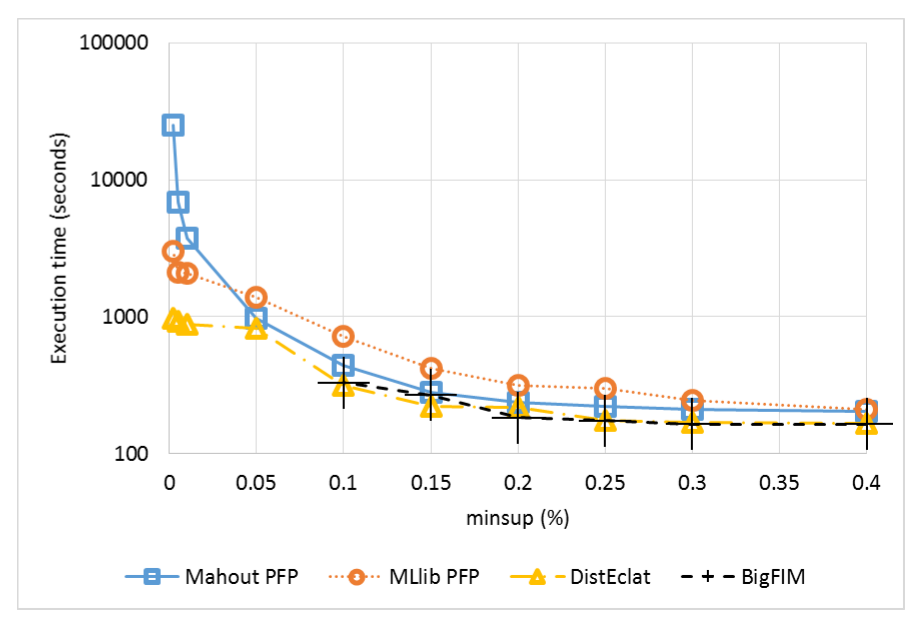
\includegraphics[width=5in]{minsup_1_log.eps}
\caption{Execution time for different $minsup$ values
(Dataset~\#1), average transaction length~10.}
\label{minsup_1}
\end{figure}


%\begin{figure}[!t]
%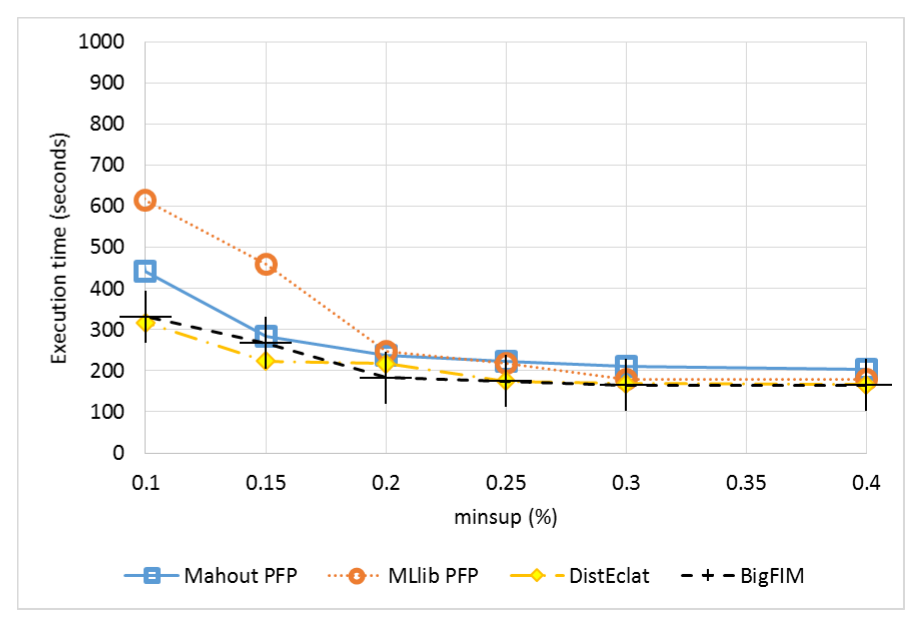
\includegraphics[width=5in]{minsup_2.eps}
%\caption{Detail of the chart in Figure~\ref{minsup_1} for high $minsup$ values (Dataset~\#1).
%[@FABIO3: da rimuovere, figura precedente ha scala logaritmica.]}
%\label{minsup_2}
%\end{figure}


\begin{figure}[!t]
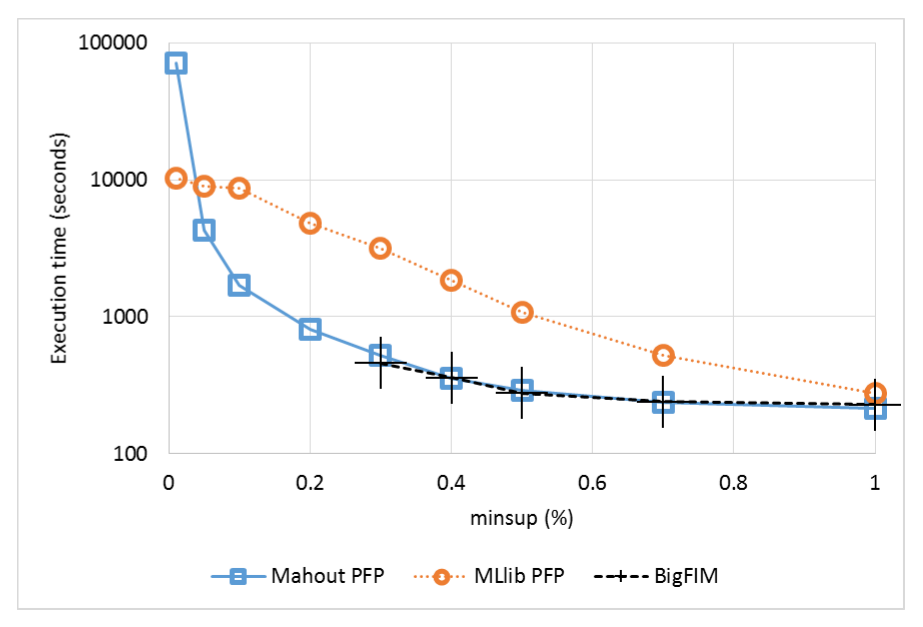
\includegraphics[width=5in]{minsup_3_log.eps}
\caption{Execution time for different $minsup$ values
(Dataset~\#3), average transaction length~30.}
\label{minsup_3}
\end{figure}



To avoid the bias due to a specific single data distribution,
two different datasets have been considered:
Dataset~\#1 and Dataset~\#3 (Table~\ref{datasets_transactions}).
They share the same average maximal pattern length (5),
the number of different items (100 thousands),
the correlation grade among patterns (0.25), and
the number of transactions (10 millions).
The difference is in the average transaction length:
10 items for Dataset~\#1 and 30 items for Dataset~\#3.
Being the other characteristics constant,
longer transactions lead to a higher dataset density,
which results into a larger number of frequent itemsets.
%Furthermore, we can test the performance degradation
%when dealing with high-dimensional datasets.


Figure~\ref{minsup_1} reports the execution time of the algorithms when varying 
the $minsup$ threshold from 0.002\% to 0.4\% and
considering Dataset~\#1. DistEclat is the fastest algorithm for all the
considered $minsup$ values. However, the improvement with respect to the
other algorithms depends on the value of $minsup$.
%When $minsup$ is greater than or equal to 0.2\%, all the implementations show
%similar performance, with BigFIM and DistEclat being slightly faster than
%Mahout PFP and MLlib PFP.
When $minsup$ is greater than or equal to 0.2\%, all the implementations show
similar performances.
The performance gap largely increases with $minsup$ values lower than 0.05\%.
%Mahout PFP becomes orders of magnitude slower than both
%DistEclat and MLlib PFP. 
BigFIM is as fast as DistEclat when $minsup$ is higher than 0.1\%, but below
this threshold BigFIM runs out of memory during the extraction of 2-itemsets.
%MLlib PFP is generally slower than Mahout PFP,
%becoming faster only for $minsup$ values below 0.05\%.
%Based on this first set of experiments, DistEclat seems to be the
%most appropriate choice, with excellent results when very low values of $minsup$ are considered,
%followed by MLlib PFP, which can reach very low $minsup$ values with
%good performance, at the expense of slightly slower performance for higher $minsup$ values.

% %In this set of experiments, different values of minimum support threshold are
% used to extract the frequent itemsets. The input datasets used are two, with two
% different transaction length: dataset \#1 with 10 items and 10 million
% transactions and dataset \#7, with 30 items and 10 million transactions
% (~\ref{datasets_transactions}).
% %With dataset \#1 and a support above 0,1 \%, all the implementations show
% similar perfomances, as shown in Figure~\ref{minsup_2}, which is an enlargement
% of the the graph in Figure~\ref{minsup_1}. Precisely, BigFIM and DistEclat prove
% to be the fastest implementations. Below this treshold, BigFIM runs out of
% memory, while Mahout PFP completes all the tasks with an execution time much
% higher than the MLlib implementation (almost 6 times).
% % %DistEclat, finally, has the best performance, completing the task with the
% % minimum wallclock time, closely followed by MLlib PFP.
% % %The experiment demostrates that DistEclat and MLlib PFP are the most reliable
% % algorithms when the minsup values start to be very low.

In the second set of experiments, we analyzed the execution time of
the algorithms for different minimum support values on Dataset~\#3,
which is characterized by a higher average transaction length
(3 times longer than Dataset~\#1),
and a larger data size on disk (4 times bigger),
with the same number of transactions (10 millions).
Since the mining task is more computationally intensive,
$minsup$ values lower than 0.01\% were
not considered in this set of experiments,
as this has proven to be a limit for most algorithms
due to memory exhaustion or too long experimental duration (days).
Results are reported in Figure~\ref{minsup_3}.
%DistEclat runs immediately out of memory
%because of the size of the input dataset,
%which is transposed in a vertical format during the first phase:
%the longer transactions prevent it from completing such step.
MLlib PFP is much slower than Mahout PFP for most $minsup$ values (0.7\% and below),
and BigFIM, as in the previous experiment,
achieves top-level performance, but cannot scale to low $minsup$ values
(the lowest is 0.3\%),
due to memory constraints during the $k$-itemset generation phase. Finally, DistEclat was not able to run because the size of the initial tidlists was already too big.\\
Overall, as expected,
DistEclat is the fastest approach when it does not run out of memory.
Mahout PFP is the most reliable implementation across almost all $minsup$ values,
even if it is not always the fastest,
sometimes with large gaps behind the top performers.
MLlib is a reasonable tradeoff choice,
as it is constantly able to complete all the tasks in a reasonable time.
%the 2nd fastest approach
%and it is able to reach the 1st or 2nd lowest $minsup$ values.
Finally, BigFIM does not present advantages over the other approaches,
being unable to reach low $minsup$ values and to provide fast executions. \\
%\textbf{Discussion:} As expected, the first phase of BigFIM is fundamental for its performance. 
%It represents the failure point when the number of candidate itemsets is too large to be stored in the main memory of the mappers. 
%At the same time, thanks to the better load balancing, given by the split of the mining in two phases balanced phases, BigFIM is able to achieve overall competitive performances (when it does not run out of memory in the first phase). Further details about load balancing behaviour can be found in Subsection \ref{load_exp}. While the failures related to mining tasks characterized by deep search space exploration was expected, 
%because of the weakness of breadth-first approach with respect to data density, for the same reasons, the good performances in terms of execution time were less expected. Probably, the competitive performances were caused by the better load balancing in the search space exploration partitioning.\\DistEclat runs easily out of memory because of the size of the input dataset,
%which is transposed in a vertical format during the first phase. 
%The longer tidlists prevent it from completing such step. Even for this algorithm, the first phase is critical. The assumption of storing almost all the input dataset in all the nodes, at the aim of saving reading phases and communication costs, revealed to be not suitable for a problem characterized by a deep search space exploration.\\
%Mahout PFP and MLlib PFP are the only algorithms
%to complete the mining tasks for all $minsup$ values.
%Precisely,
%Mahout PFP is the most suitable technique
%when dealing with minsup values over 0.05\%,
%with a perfomance 6 to 8 times faster than the MLlib sibling.
%However, with lower $minsup$ values,
%Spark MLlib becomes the fastest approach with an order of magnitude gap.
%We identified the cause of the different performance
%between the two PFP implementations
%in the different pruning strategies.
%The algorithms which extract closed itemsets, such as Mahout PFP,
%can apply more effective pruning techniques
%that are not applicable when all frequent itemsets must be extracted,
%which is the case for MLlib PFP.
%When the problem becomes deeper and more challenging, beyond the engineering differences between the two implementations, the better load balancing of the MLlib PFP makes it faster.

%their different mining phases: even if both of them extracts the same set of itemset in this specific use cases, the extraction process is different because MLlib PFP extracts all the frequent itemsets. Mahout PFP, instead, extracts only the closed ones\footnote{The differences are not reported in the paper.}.
%the Spark implementation extracts all the frequent itemsets and then selects the closed ones,
%while the Hadoop implementation directly extracts only the closed frequent itemsets.





% %Indeed, we can say that DistEclat and MLLib are the best approaches for
% different $minsup$ values analyses but are strongly affected, respectively, by
% dataset size and transaction length. When one of these features increases,
% Mahout PFP is the only algorithm able to complete the tasks.

%\begin{table*}[h!]
%\begin{center}
%\caption{Synthetic datasets used for different transaction length experiments}
%\label{datasets_attributes}
%\begin{tabular}{|c|c|c|c|c|}
%\hline
%{\bf ID }& {\bf IBM Generator} &  {\bf \# different } & {\bf  \# items  } & {\bf size} \\
%{\bf  }& {\bf  parameters } &  {\bf items  } & {\bf per } & {\bf (GB) } \\
%{\bf  } & {\bf } & {\bf } & {\bf  transaction } & {\bf } \\ \hline
% \hline
%6  & T20P5I100kC0.25D10000k  & 18011 & 29.99 & 1187 \\ \hline
%7  & T30P5I100kC0.25D10000k  & 18011 & 29.99 & 1776 \\ \hline
%8 & T40P5I100kC0.25D10000k  & 18010 & 39.98 & 2364 \\ \hline
%9 & T50P5I100kC0.25D10000k  & 18014 & 49.98 & 2953 \\ \hline
%10 & T60P5I100kC0.25D10000k  & 18010 & 59.98 & 3541 \\ \hline
%11 & T70P5I100kC0.25D10000k  & 18016 & 69.98 & 4130 \\ \hline
%12 & T80P5I100kC0.25D10000k  & 18012 & 79.98 & 4719 \\ \hline
%13 & T90P5I100kC0.25D10000k  & 18014 & 89.97 & 5307 \\ \hline
%14 & T100P5I100kC0.25D10000k & 18015 & 99.97 & 5896 \\ \hline
%\end{tabular}
%\end{center}
%\end{table*}



%\begin{table*}[h!]
%\begin{center}
%\caption{Synthetic datasets used for different pattern lengths}
%\label{datasets_patterns1}
%\begin{tabular}{|c|c|c|c|c|c|}
%\hline


%{\bf ID }& {\bf IBM Generator parameters } & {\bf Number of } & {\bf Average number of } & {\bf size} \\
%{\bf  } & {\bf } & {\bf different items } & {\bf items per transaction } & {\bf } \\ \hline
% \hline
%15 & T20P2I100kC0.25D10000k  & 8212 & 19,99 & 1.188 \\ \hline
%16 & T20P4I100kC0.25D10000k & 14976 & 19,99 & 1.187 \\ \hline
%17 & T20P6I100kC0.25D10000k  & 20727 & 19,99 &1.187 \\ \hline
%18 & T20P8I100kC0.25D10000k & 25864 & 20,03 &1.188 \\ \hline
%19 & T20P10I100kC0.25D10000k & 30215 & 20,09 &1.192 \\ \hline
%20 & T20P12I100kC0.25D10000k &  34233 & 20,26 &1.202 \\ \hline
%21 & T20P14I100kC0.25D10000k &  37672 & 20,56 & 1.221 \\ \hline
%22 & T20P16I100kC0.25D10000k &  40955 & 21,04 & 1.249 \\ \hline
%
%\end{tabular}
%\end{center}
%\end{table*}






%\begin{table*}[]
%\begin{center}
%\caption{Synthetic datasets used for different pattern lengths}
%\label{datasets_patterns2}
%\begin{tabular}{|c|c|c|c|c|c|}
%\hline
%{\bf ID }& {\bf IBM Generator parameters } & {\bf Number of transactions } & {\bf Number of } & {\bf Average number of } & {\bf size} \\
%{\bf  }& {\bf } & {\bf } & {\bf different items } & {\bf items per transaction } & {\bf } \\ \hline
% \hline
%22 & T40P2I100kC0.25D10000k & 10.000.000 & 8215 & 39,99 & 2,4 GB \\ \hline
%23 & T40P4I100kC0.25D10000k & 10.000.000 & 14,979 & 39,99 & 2,4 GB \\ \hline
%24 & T40P6I100kC0.25D10000k & 10.000.000 & 20733 & 39,98 & 2,4 GB \\ \hline
%25 & T40P8I100kC0.25D10000k & 10.000.000 & 25864 & 39,98 & 2,4 GB \\ \hline
%26 & T40P10I100kC0.25D10000k & 10.000.000 & 30220 & 39,99 & 2,4 GB \\ \hline
%27 & T40P12I100kC0.25D10000k & 10.000.000 & 34262 & 39,98 & 2,4 GB \\ \hline
%28 & T40P14I100kC0.25D10000k & 10.000.000 & 37673 & 39,98 & 2,4 GB \\ \hline
%29 & T40P16I100kC0.25D10000k & 10.000.000 & 40971 & 39,98 & 2,4 GB \\ \hline
%\end{tabular}
%\end{center}
%\end{table*}


%%
%%\begin{table*}[h!]
%%\begin{center}
%%\caption{Experimental result summary for $minsup$ impact, Section~\ref{minsup_exp}}
%%\label{minsup_resume}
%%\begin{tabular}{|c|c|c|c|c|}
%%\hline
%%\textbf{}          & \multicolumn{2}{l|}{\textbf{Transaction length: 10}} & \multicolumn{2}{l|}{\textbf{Transaction length: 30}} \\ \hline
%%\textbf{algorithm} & \textbf{lowest $minsup$}        & \textbf{speed}        & \textbf{lowest $minsup$}        & \textbf{speed}        \\ \hline
%%Mahout PFP         & 0.002 \%                       & 3rd                  & 0.01 \%                         & 2nd                 \\ \hline
%%MLlib PFP          & 0.002 \%                       & 2nd                  & 0.01 \%                         & 1st                  \\ \hline
%%BigFIM             & 0.1 \%                         & 4th        	   & 0.3 \%                         & 3rd                  \\ \hline
%%DistEclat          & 0.002 \%                       & 1st                  & -                              & -                    \\ \hline
%%\end{tabular}
%%\end{center}
%%\end{table*}
%%




\subsection{Impact of the average transaction length}
\label{attributes_exp}

\begin{figure}[!t]
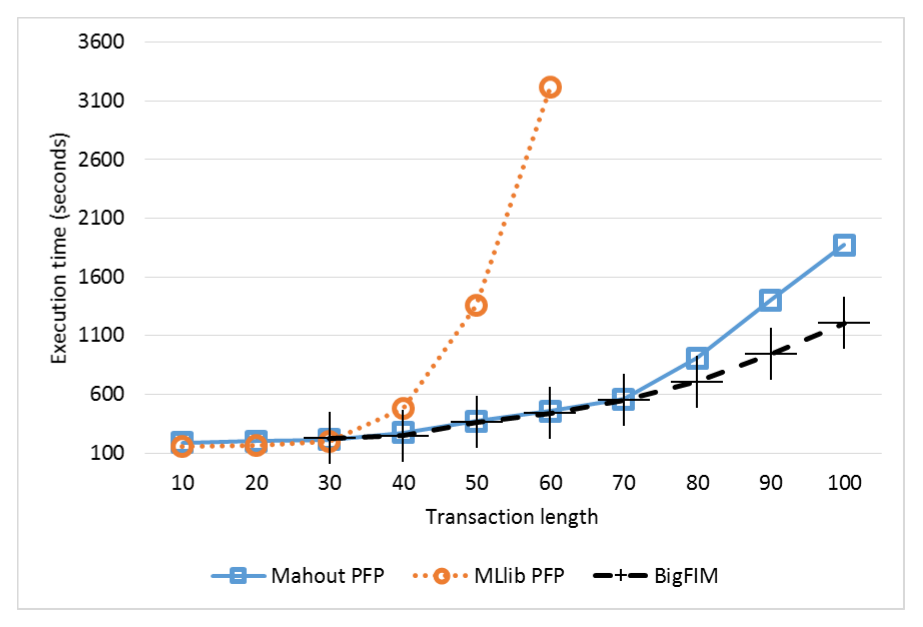
\includegraphics[width=5in]{attributes.eps}
\caption{Execution time with different average transaction lengths % with a minsup value of 1\%
(Datasets \#1--10, $minsup$ 1\%).}
\label{attributes}
\end{figure}

\begin{figure}[!t]
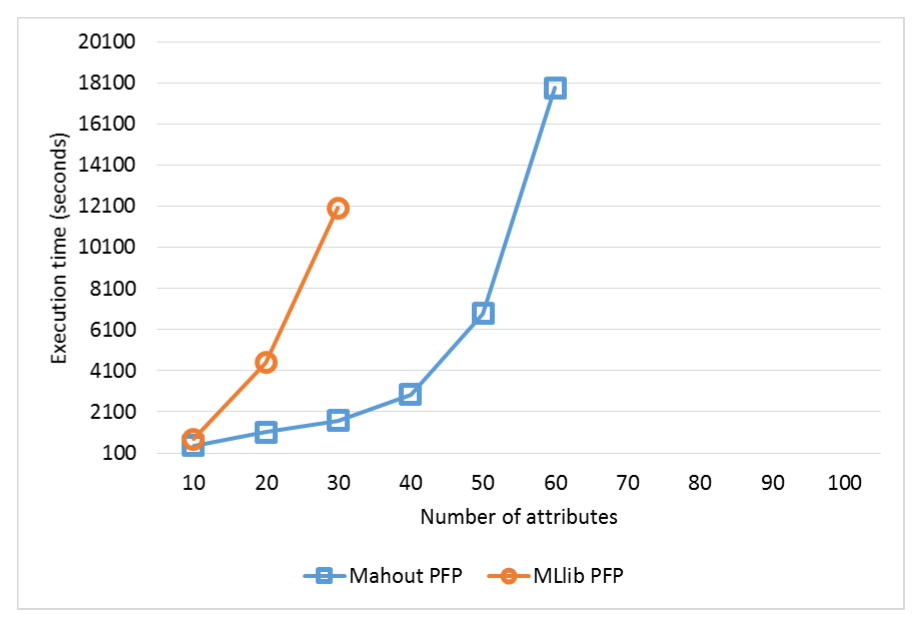
\includegraphics[width=5in]{attributes_deeper.eps}
\caption{Execution time with different average transaction lengths %with a minsup value of 0.1\%
(Datasets \#1--10, $minsup$ 0.1\%).}
\label{attributes_deeper}
\end{figure}

We analyzed the effect of different average transaction lengths,
from 10 to 100 items per transaction.
We fixed the number of transactions to 10 millions.
To this aim, Datasets \#1--10 were used (see Table~\ref{datasets_transactions}).
Longer transactions often lead to more dense datasets and a larger number of long frequent itemsets.
This generally corresponds to more computationally intensive tasks.
The execution times obtained are reported in Figure~\ref{attributes} and Figure~\ref{attributes_deeper}, with a respective {\it minsup} value of 1\% and 0.1\%.
In the experiment of Figure~\ref{attributes}, BigFIM and DistEclat execution times for transaction length of 10 and 20 are not reported because, for these configurations, no 3-itemsets are extracted and hence the two algorithms crashed\footnote{Due to the absence of a specific test, BigFIM and DistEclat crash
if no itemsets longer than the value of the prefix length parameter are mined.}.
For higher transaction lengths, DistEclat is not included since it runs out of memory
for values beyond 20 items per transaction.
The other algorithms have similar execution times for short transactions,
up to 30 items.
For longer transactions, a clear trend is shown:
(i) MLlib PFP is much slower than the others
and it is not able to scale for longer transactions,
as its execution times abruptly increase until it runs out of memory;
(ii) Mahout PFP and BigFIM have a similar trend until 70 items per transactions,
when Mahout PFP becomes slower than BigFIM.\\
The experiments of Figure~\ref{attributes_deeper}, shows a very similar trend, with exception that also BigFIM is not able to run.\\
Overall, despite the Apriori-based initial phase,
BigFIM proved to be the best scaling approach for very long transactions and a relatively high minsup. When the minsup is decreased only Mahout PFP 
is able to cope with the complexity of the task.\\
%\textbf{Discussion:} As expected (see Figure~\ref{attributes_deeper}), for more dense data distributions the number of candidate itemsets increases and BigFIM runs out of memory due to its initial Apriori phase. 
%A similar motivation holds for DistEclat failures, due to its requirement to store all the (longer) tidlists in all the nodes.
%The FP-growth based approaches are affected by the increasing length of the transactions. However, their depth-first structure revealed to be the best exploration strategy in such an environment (i.e. high number of attributes). 
%DistEclat leverages a depth-first exploration strategy as well, however it assumes that all the tidlists should be stored in all the commodity cluster nodes, which is challenging if considering the further memory requirements due to the search space exploration. 
%The difference gap between the two PFP implementations might be related to the different pruning strategies.


%Despite the Apriori-based initial phase, BigFIM shows to be the mo
%PFP is not optmized to address long transactions due to its FP-tree structure,
%whereas BigFIM is able to address denser data distributions and a large
%number of attributes.


%\begin{table*}[h!]
%\begin{center}
%\caption{Experimental result summary for transaction length impact, Section~\ref{attributes_exp}}
%\label{transaction_length_resume}
%\begin{tabular}{|c|c|c|}
%\hline
%
%\textbf{algorithm} & \textbf{reached transaction length}        & \textbf{speed}        \\ \hline
%BigFIM             & 100                        & 1st        	                  \\ \hline
%Mahout PFP         & 100                       & 2nd                          \\ \hline
%MLlib PFP          & 60                       & 3rd                                 \\ \hline
%DistEclat          & -                       & -                            \\ \hline
%\end{tabular}
%\end{center}
%\end{table*}
%


% % COMMENTO A FIGURA 5 RIMOSSA
% In order to assess this type of experiments with the ones of the Section
% \ref{minsup_exp}, we have performed a set of experiments dealing with datasets
% of both a varying transaction length (focusing on datasets with an average
% number of items from 10 to 30) and different minsup values (0.01\% and 0.05\%).
% % %We also performed a set of experiments with the same datasets lowering the
% % minimum support threshold (we considered $minsup$=0.01\% and $minsup$=0.05\%) .
% The results are reported in Figure \ref{attributes_2}.  The execution time of
% BigFIM is not reported because, as already evidenced in Section
% \ref{minsup_exp},  it is unable to complete the mining task when
% low values of minsup are considered. On the other hand, different performances
% of Mahout PFP and MLlib PFP are noticeable. When the $minsup$ is 0.05\% Mahout
% PFP is
% still faster than MLlib PFP. Indeed, when the $minsup$ value is 0.01\% MLlib
% becomes faster
% than Mahout PFP. Hence, this results confirm that MLlib is the best approach
% when dealing with very low $minsup$ values.




% %The difference between the performance of Mahout PFP and MLlib PFP, as before,
% may be caused by the difference mining processes. Since Mahout PFP
% %mines only the frequent closed itemsets, it can exploit more effective pruning
% techniques and reduce the depth of the recursive mining phase. Differently,
% %MLlib PFP, which mines all the frequent itemsets, has a deeper recursive mining
% phase, in particular when long transactions are considered.
% %The difference between the performance of Mahout PFP and MLlib PFP, as before,
% may be caused by the difference mining processes which lead to different type
% %of outputs, even if, in this specific case, the number of frequent itemsets
% matches the number of closed ones.



% \begin{figure}[!t]
% 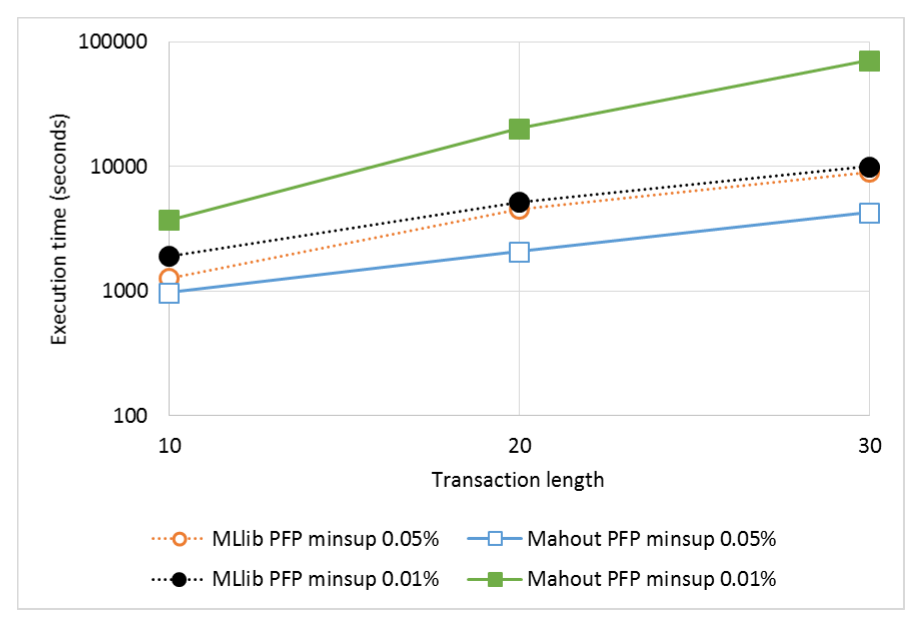
\includegraphics[width=5in]{attributes_2.eps}
% \caption{Execution time with different average transaction lengths,
% and $minsup$ values 0.01\% and 0.05\%.}
% \label{attributes_2}
% \end{figure}



% %ELIMINARE DA QUI
% %The second set of experiments studies the performance of the approaches dealing
% with datasets obtained setting different expected frequent patterns length. We
% utilised a configuration with 20 attributes and another with 40 (respectively
% detailed in tables ~\ref{datasets_patterns1} and ~\ref{datasets_patterns2}) with
% different expected patterns length. Therefore, the datasets of these evaluation
% differ for their density. A higher expected pattern length is typical of dense
% dataset distributions, while sparse datasets are characterised by many short
% itemsets.
% %The minsup value is set to 0,25\% for the first set of experiments and to
% 0,40\% for the second one. We changed the minsup values in order to have
% significative output and a good number of approaches that not run out of memory.
% %
% %In the first case, DistEclat was able to run even if it showed memory issues
% for the longest expected patterns, as illustrated in the graph in
% Figure~\ref{pattern_small}. Even in this experiment, BigFIM performances
% revealed to be the most stable of the set of algorithms for all the pattern
% length configurations, even if Mahout PFP is not far. MLlib implementation is
% able to execute all the tasks, but it shows a serious gap when the expected
% patterns are short. This is very interesting, because one can expect a behaviour
% more similar to the one of the previous experiment, where the execution time
% strongly increases together with the average transaction length of the input
% dataset. Clearly, the perforamance related to the average length of transactions
% and the average length of the expected patterns are not correlated.
% %We counted the frequent itemsets produced to understand if the performance
% degradation was reasoned by an explosion of the number of itemsets. As repored
% in Table~\ref{extracted_itemsets}, this was not the case.
% %
% %In the second case, with an average transaction length of 40 items and a minsup
% of 0,4\%, the behaviour of the algorithms is very similar, except for DistEclat
% that is not able to mine the input. BigFIM shows the best performance followed
% by Mahout PFP, which has apeak corresponding to an expected pattern length of
% 14. The behaviour is similar to the previous experiment, in which it was less
% explicit. In these cases, the number of extracted itemset is much higher than
% the previous case, as shown in Table~\ref{extracted_itemsets}. Above all, the
% high execution time is caused by a not proper load balancing. In fact, almost
% all the tasks of the mining MapReduce job of the process finish the computation
% below a minute of wall clock time, one of them reaches 3 minutes while the last
% 2 last respectively take over 8 minutes and over 32 minutes. This validates the
% assumption about Mahout PFP load balancing in subSection ~\ref{FP-Growth}.
%




%\begin{table*}[h!]
%\begin{center}
%\caption{Synthetic datasets used for different pattern lengths}
%\label{datasets}
%\begin{tabular}{|c|c|c|c|c|c|}
%\hline
%
%ID & IBM Generator  & Number of  & Number of  & Average number & size\\
% & parameters & transactions & different & of items per & \\
% & &  &  items & transaction &\\ \hline
%14 & T20P2I100kC0.25D10000k & 10.000.000 & 8212 & 19,99 & 1,2 GB \\ \hline
%15 & T20P4I100kC0.25D10000k & 10.000.000 & 14976 & 19,99 & 1,2 GB \\ \hline
%16 & T20P6I100kC0.25D10000k & 10.000.000 & 20727 & 19,99 & 1,2 GB \\ \hline
%17 & T20P8I100kC0.25D10000k & 10.000.000 & 25864 & 20,03 & 1,2 GB \\ \hline
%18 & T20P10I100kC0.25D10000k & 10.000.000 & 30215 & 20,09 & 1,2 GB \\ \hline
%19 & T20P12I100kC0.25D10000k & 10.000.000 & 34233 & 20,26 & 1,2 GB \\ \hline
%20 & T20P14I100kC0.25D10000k & 10.000.000 & 37672 & 20,56 & 1,2 GB \\ \hline
%21 & T20P16I100kC0.25D10000k & 10.000.000 & 40955 & 21,04 & 1,2 GB \\ \hline
%
%\end{tabular}
%\end{center}
%\end{table*}
%
%\begin{table*}[h!]
%\begin{center}
%\caption{Synthetic datasets used for different pattern lengths}
%\label{datasets}
%\begin{tabular}{|c|c|c|c|c|c|}
%\hline
%
%ID & IBM Generator  & Number of  & Number of  & Average number & size\\
% & parameters & transactions & different & of items per & \\
% & &  &  items & transaction &\\ \hline
%22 & T40P2I100kC0.25D10000k & 10.000.000 & 8215 & 39,99 & 2,4 GB \\ \hline
%23 & T40P4I100kC0.25D10000k & 10.000.000 & 14,979 & 39,99 & 2,4 GB \\ \hline
%24 & T40P6I100kC0.25D10000k & 10.000.000 & 20733 & 39,98 & 2,4 GB \\ \hline
%25 & T40P8I100kC0.25D10000k & 10.000.000 & 25864 & 39,98 & 2,4 GB \\ \hline
%26 & T40P10I100kC0.25D10000k & 10.000.000 & 30220 & 39,99 & 2,4 GB \\ \hline
%27 & T40P12I100kC0.25D10000k & 10.000.000 & 34262 & 39,98 & 2,4 GB \\ \hline
%28 & T40P14I100kC0.25D10000k & 10.000.000 & 37673 & 39,98 & 2,4 GB \\ \hline
%29 & T40P16I100kC0.25D10000k & 10.000.000 & 40971 & 39,98 & 2,4 GB \\ \hline
%\end{tabular}
%\end{center}
%\end{table*}




\subsection{Impact of the number of transactions}
\label{transaction_exp}

\begin{figure}[!t]
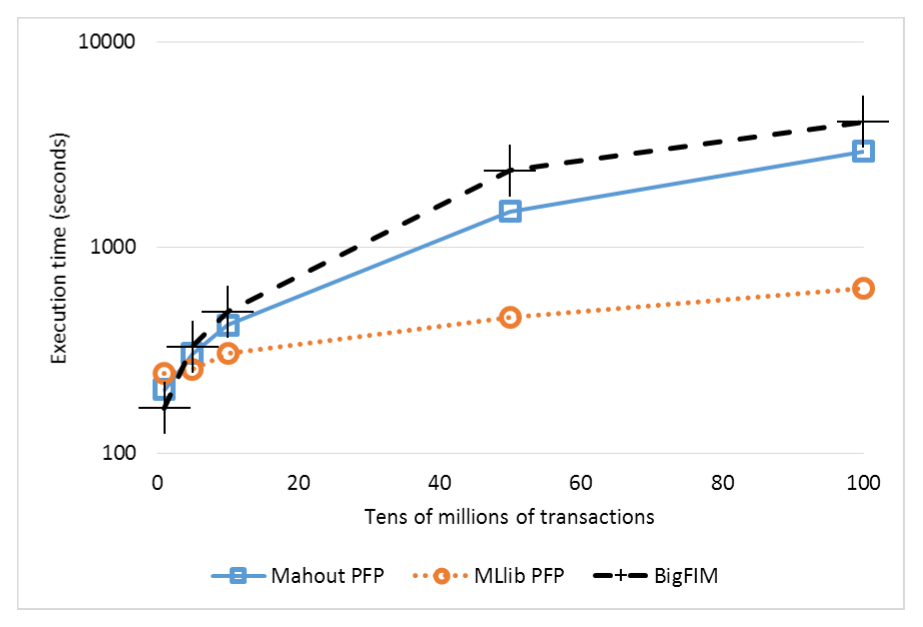
\includegraphics[width=5in]{transactions_log.eps}
\caption{Execution time with different numbers of transactions
 (Datasets \#1, \#11--14,
 $minsup$~0.4\%).}
\label{transactions}
\end{figure}

We evaluated the effect of varying the number of transactions,
i.e., the dataset size, without changing intrinsic data characteristics (e.g., 
transaction length or data distribution).
The experiments have been performed on Datasets \#1, \#11--14 have been used
(see Table~\ref{datasets_transactions}),
which have a number of transactions
ranging from 10 millions to 1 billion.
The $minsup$ is set to 0.4\%,
which is the highest value for which the mining leverages both phases of
BigFIM, and it corresponds to the highest value used
in the experiments of Section~\ref{minsup_exp}.
Since in the experiment the relative minsup threshold is fixed, from the mining point of view, the search space exploration is similar and not particularly challenging, as shown in Section~\ref{minsup_exp}. What really affects this experiment is the algorithms reliability dealing with such amounts of data.

As shown in Figure~\ref{transactions}, all the considered algorithms scale
almost linearly with respect to the dataset cardinality, with BigFIM being the slowest,
closely followed by Mahout PFP,
and with MLlib PFP being by far the fastest approach,
with execution times reduced by almost an order of magnitude. 
PFP implementations are faster than BigFIM because they read from the disk the input dataset only twice. 
BigFIM pays the iterative disk reading activities during its initial Apriori phase when the number of records
of the input dataset increases.
Finally, DistEclat fails under its assumption that the tidlists of the entire dataset should
be stored in each node, and it is not able to complete the extraction beyond
10 million transactions.
%This experiment, because of the size of the involved input dataset, should be very related to the behavior in terms of communication costs of the algorithms. As we will detail in Subsection~\ref{communication_costs}, Mahout PFP implemention is, by far, the algorithm assuming less data across the network. However, in this experiment, the performance of Mahout PFP are not the best-in-class. For the same reason, even the gap with the performances of BigFIM is not that large (since the communication costs balance differs, instead, by a factor larger than four).
%\begin{table*}[h!]
%\begin{center}
%\caption{Experimental result summary for number of transactions impact, Section~\ref{transaction_exp}}
%\label{transaction_resume}
%\begin{tabular}{|c|c|c|}
%\hline
%
%\textbf{algorithm} & \textbf{reached dataset size}        & \textbf{speed}      \\
%\textbf{algorithm} & \textbf{tens of millions of transactions}        &      \\ \hline
%MLlib PFP          & 100                       & 1st                               \\ \hline
%Mahout PFP         & 100                       & 2nd                          \\ \hline
%BigFIM             & 100                        & 3rd       	                  \\ \hline
%DistEclat          & 1                       &  -                            \\ \hline
%\end{tabular}
%\end{center}
%\end{table*}








\subsection{Scalability in terms of parallelization degree}
\label{nr_machines}



\begin{figure*}[!t]
\begin{center}
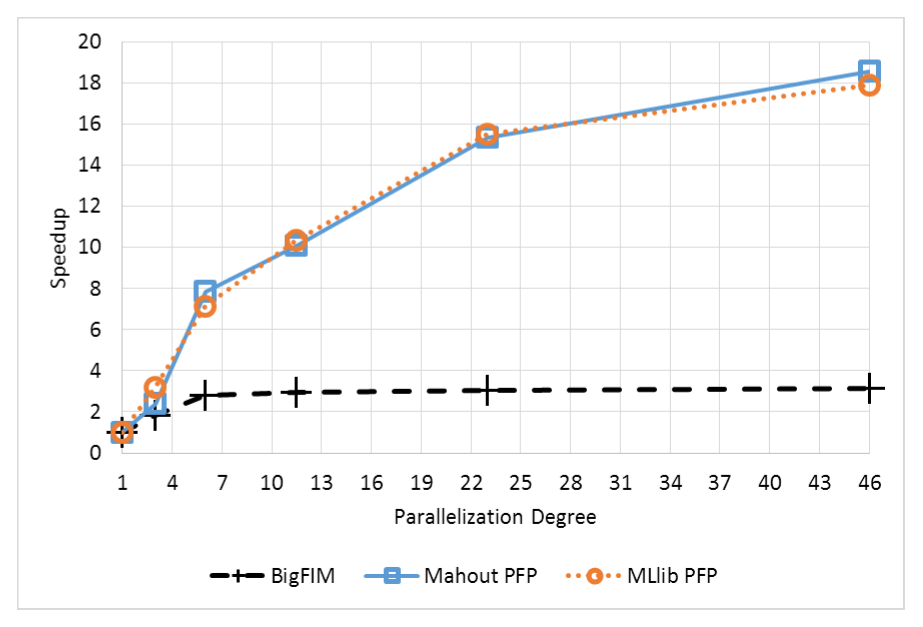
\includegraphics[width=5in]{machines_big.eps}
\caption{Speedup with different parallelization degrees (Dataset \#14,
 $minsup$~0.4\%)}
\label{nr_machines_speedup}
\end{center}
\end{figure*}


%\begin{figure*}[!t]
%\begin{center}
%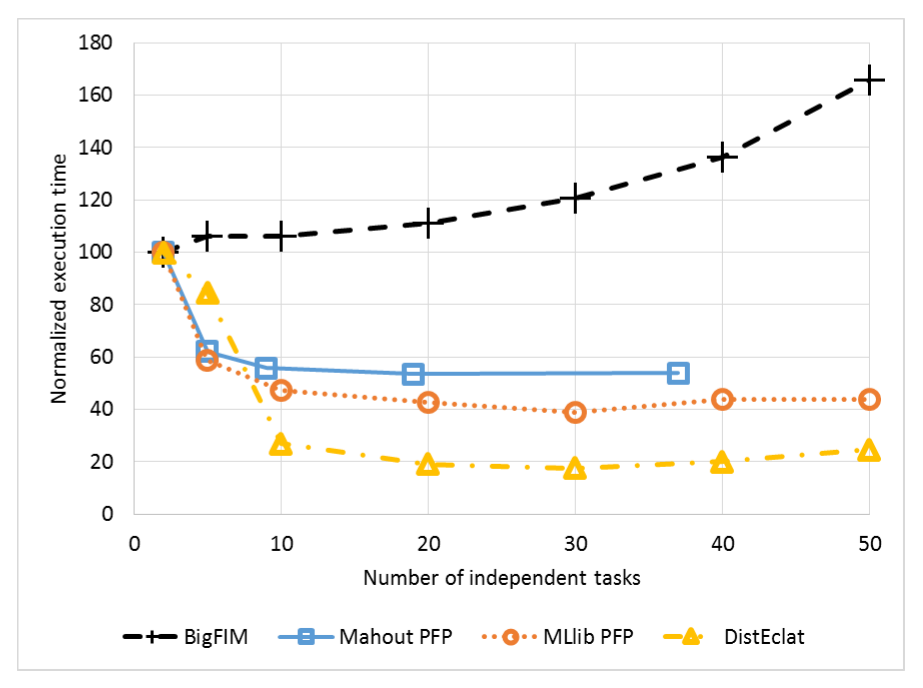
\includegraphics[width=5in]{machines_2.eps}
%\caption{Normalized execution time with different number of machines  (Dataset \#1,
% $minsup$~0.11\%,
% average transaction length~10) \textbf{Qui BigFIM va proprio male, mi chiedo se sia il caso di eliminare questo esperimento (ma perderemmo disteclat)}}
%\label{nr_machines_2}
%\end{center}
%\end{figure*}

We analyzed the speedup by running the same mining problem with increasing numbers of parallel tasks.
The dataset selection and the $minsup$ parameter choice are difficult 
since we need to identify a mining problem satisfying two conditions:
(i) allowing all the executions to complete with any number of parallel tasks, 
and, at the same time, 
(ii) being very demanding so that the distributed framework is actually exploited. 
We selected $minsup$ 0.4\% and Dataset \#14 (see Table~\ref{datasets_transactions}) 
to be light enough for condition (i) and demanding enough for condition (ii).

Figure~\ref{nr_machines_speedup} shows the speedup results. 
A parallelization degree equal to 1 corresponds to the minimal computational resource setting, i.e., the configuration with only two parallel independent tasks.
Its execution time is the reference with respect to which the speedup is computed. 
Specifically, the speedup of a configuration with a parallelization degree equal to $p$ is computed as 

$$speedup(paral\_degree=p)=\frac{Exec\_Time(paral\_degree=1)}{Exec\_Time(paral\_degree=p)}$$ 

Ideally, the speedup should be equal to the parallelization degree $p$ itself, i.e., 
increasing the number of resources (parallel tasks) of a factor $p$, should lead to a speedup equal to $p$.
%In Figure~\ref{nr_machines_speedup}, the execution time of the basic configuration are divided by the ones related to the higher degree of parallelization to obtain the speedup values.
 % (Figure~\ref{nr_machines_1}). 
%Since the problem was already too challenging for a single task, we have started from 2. In Figure~\ref{nr_machines_1} and Figure~\ref{nr_machines_speedup} are shown the performance of the algorithms leveraging different parallelization degree values.
% In In Figure~\ref{nr_machines_1}, the execution times are normalized with respect with the execution time obtained with the time obtained with the base number of machines (i.e. 2).
% ( $T_{old}/T_{new}$ ).
%for different multiplicative factors of computation improvement (since the basic parallelization degree is 2, the number of independent tasks in the x axis can be obtained by multiplying times 2)     \footnote{Please note that the Mahout-PFP curve in Figure~\ref{nr_machines_1} appears shifted with respect to the others because of the following reason. This specifical implementation does not allow to control the numbers of mappers involved in the computation, therefore we had to change input chunk size. This value allowed us to force a fixed set of possible configurations. }. 

In this experiment, it is clear that the FP-Growth-based implementations provide a better speedup. 
BigFIM, on the contrary, is not able to leverage a number of parallel tasks higher than 6.
% However, only MLlib PFP has a speedup that is close to the ideal one.
Because of the size of the dataset, DistEclat is not able to perform the mining. 
%In the previous experiments, it has demonstrated to be reliable only with mining requiring less than few minutes \footnote{Considering just the experiments in which all the algorithms complete the mining}. Repeating the same kind of scalability experiment for a mining of few minutes is not sensed because the parallelization overheads likely dominate the computation.\\
%
%Since DistEclat is not able to run this experiment, we used a smaller input file (Dataset \#1) and an even lower minsup value (0.11\%) (Figure~\ref{nr_machines_2}). Even in this case, the Breadth-first approaches (DistEclat) showed a very good scalability. BigFIM demonstrated again to have serious problems of scalability. In this experiment, in fact, the problem configuration is such that the best execution times is provided with the smaller number of computing nodes. Actually, the mining phase is quite fast (about 6 minutes), with a concrete possibility, hence, to be dominated by distribution overheads, especially with Apriori iterative nature. However, a slightly deeper minsup value leads to memory issue.\\
%\textbf{Discussion:}
%Based on the results it is clear that many of the considered algorithms are not able to properly exploit the parallelism provided by distributed frameworks. The reason 
%is probably given by the fact that they are not able to split the initial problem in a number of subproblems equal to the number of available parallel 
%tasks, or, when they are able to do so, the overhead given by the instance of the subtasks is greater than the advantages given by the parallel execution 
%of the subtasks/subproblems. 
%MLlib PFP has demonstrated to be the best approach, probably because of a finest granularity in the projection of the FP-trees than the other FP-growth-based approaches (the more are the independent subproblems generated, the better could be distributed to a high number of nodes). 
%Based on the results it is clear that many of the considered algorithms are not able to properly exploit the parallelism provided by Hadoop. The reason 
%is probably given by the fact that they are on able to split the initial problem in a number of subproblems equal to the number of available parallel 
%tasks, or when they are able to do it, the overhead given by the instance of the subtasks is greater than the advantages given by the parallel execution 
%of the subtasks/subproblems. MLlib PFP has demonstrated to be the best approach, probably because of a finest granularity in the projection of the FP-trees than the other FP-growth-based approaches (the more are the independent subproblems generated, the better could be distributed to a high number of nodes). 




%In this Section, as predictable, it is clear that the benefits of the parallelization is strongly mitigate after few tens of tasks. MLlib PFP has demonstrated to be the best approach, probably because a finest granularity in the projection of the FP-trees than the other approaches tree structures (the more are the independent structures to be mined, the better could be distributed to a high number of nodes). 
%The motivations behind this difficulties are related to the Frequent itemset mining problem, which is hardly parallelizzable. The partitions to which the problem is divided into often overlap. This leads to an overall load which is higher than load of an hypothetical centralized execution. For this reason, when the exploration of the search space deepen, the overlapping of the subproblems increases and the performances do not scale as desirable. 
%\textbf{(ANCHE QUI FORSE POTREMMO ENFATIZZARE IL FATTO CHE PURTROPPO IN QUESTO DOMINIO SI SCALA DAVVERO POCO. NON CONTINUARE A GUADAGNARE ALL'INFINITO E' LA NORMA, MA QUI ANCHE PROBLEMI MOLTO GRANDI SI FERMANO DOPO QUALCHE DECINE DI MACCHINE. CI POTREMMO ALLACCIARE ALLE RIFLESSIONI FINALI IN CUI DICIAMO CHE SI VEDE CHE QUESTI SONO PORTING E NESSUNO E' STATO DAVVERO PROGETTATO PER ANDARE DIRETTAMENTE PARALLELO.}


\subsection{Real use cases}
\label{usecases}

In the following, we analyze the performance of the mining algorithms in two
real-life scenarios:
(i) URL tagging of the Delicious dataset and
(ii) network traffic flow analysis.
The characteristics of the two datasets
are reported in Table~\ref{datasets_real}.

\begin{table*}[h!]
\scriptsize
\begin{center}
\caption{Real-life use-cases dataset characteristics}
\label{datasets_real}
\begin{tabular}{|c|c|c|c|c|c|}
\hline
{\bf ID }& {\bf Name} 	&  {\bf Num. of} 	& {\bf  Avg. \# items} 			& {\bf Size} \\
{\bf  }& {\bf  } 		&  {\bf different items} 	& {\bf  per transaction} 	& {\bf (GB) } \\
\hline
\hline
15& Delicious & 57,372,977 & 4 & 44.5 \\ \hline
16 & Netlogs & 160,941,600 & 15 & 0.61  \\ \hline
\end{tabular}
\end{center}
\end{table*}





\subsubsection{URL tagging}
\label{delicious_exp}

We evaluated the selected algorithms on the Delicious dataset~\cite{wetzker2008analyzing}, which is a
collection of web tags.
Each record represents the tag assigned by a user to a URL and it consists of
4 attributes:
date,
user id (anonymized),
tagged URL,
and tag value.
The transactional representation of the Delicious dataset includes
one transaction for each record, where each transaction is a set of four pairs
(attribute, value), i.e., one pair for each attribute.
The dataset stores more than 3 years of web tags.
It is very sparse because of the huge number of different URLs
and tags.
Additional characteristics of the dataset are reported
in Table~\ref{delicious_itemsets}.

This experiment simulates the environment of a service provider that
periodically analyzes the web tag data to extract frequent patterns: they
represent the most frequent correlations among tags, URLs, users, and dates.
Many different use cases can fit this description:
tag prediction, topic classification, trend evolution, etc.
Their evolution over time is also interesting.
To this aim, the frequent itemset extraction has been executed
cumulatively on temporally adjacent subsets of data,
whose length is a quarter of year (i.e., first quarter,
then first and second quarter, then first, second, and third quarter, and so on,
as if the data were being colleted quarterly and analyzed as a whole at the
end of each quarter).
The setting of $minsup$ in a realistic use-case proved to be a critical choice.
Too low values lead to millions of itemsets,
which become useless as they exceed the human capacity to understand the results.
However, too high $minsup$ values would discard longer itemsets,
which are more meaningful
as they better highlight more complex correlations
among the different attributes and values.
Because of the high sparsity of the dataset,
we identified the setting $minsup$=0.01\% as the best tradeoff.

\begin{table}[h]
\scriptsize
\begin{center}
\caption{Delicious dataset: cumulative number of transactions and frequent itemsets
with $minsup$~0.01\%.}
\label{delicious_itemsets}
\begin{tabular}{|c|c|c|c|}
\hline
{\bf Up to year,}	& {\bf Number of} 	& {\bf	Number of} \\
{\bf month, quarter}	& {\bf transactions} 	& {\bf	frequent itemsets} \\
\hline \hline
2003 Dec, Q4 	& 153,375	 	& 7197 \\ \hline
2004 Mar, Q1  	& 489,556		& 6013 \\ \hline
2004 Jun, Q2	& 977,515		& 5268 \\ \hline
2004 Sep, Q3 	& 2,021,261		& 5084 \\ \hline
2004 Dec, Q4 	& 4,349,209		& 4714 \\ \hline
2005 Mar, Q1	& 9,110,195		& 4099 \\ \hline
2005 Jun, Q2	& 15,388,516		& 3766 \\ \hline
2005 Sep, Q3	& 24,974,689		& 3402 \\ \hline
2005 Dec, Q4	& 41,949,956		& 3090 \\ \hline
\end{tabular}
\end{center}
\end{table}

\begin{figure}[!t]
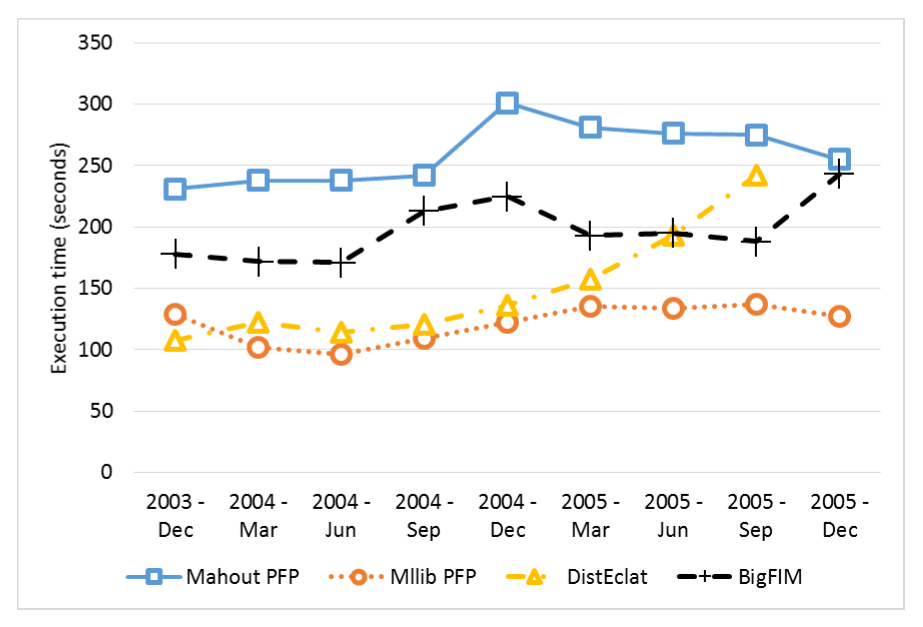
\includegraphics[width=5in]{delicious.eps}
\caption{Execution time for different periods of time on the Delicious dataset
($minsup$=0.01\%)}
\label{delicious}
\end{figure}


Table~\ref{delicious_itemsets} reports the cumulative number of
transactions for the different periods of time
(i.e., the cardinality of the input dataset) and the
number of frequent itemsets extracted with a fixed $minsup$ of 0.01\%,
while the execution times of the
different algorithms are shown in Figure~\ref{delicious}.


MLlib PFP consistently proves to be the fastest approach, with DistEclat following.
However, while DistEclat is slightly faster than MLlib PFP only with the first, smallest dataset
(up to Dec 2003, with 150 thousands transactions), when the dataset size increases,
DistEclat execution time does not scale. DistEclat eventually fails for the final
40-million-transaction dataset of Dec 2005, due to memory exhaustion.
BigFIM and Mahout PFP consistently provide 2 to 3 times higher execution times.
Apart from DistEclat, all algorithms complete the task with similar performance
despite increasing the dataset cardinality from 150 thousand transactions to 41 millions,
thanks to the constant relative $minsup$ threshold
which reduces the number of frequent itemsets
for decreasing density of the dataset.
Hence, MLlib PFP is the best choice for this dataset characterized by short transactions
(the transaction length is 4).


% %Therefore, we extracted the frequent itemset related to an incremental period
% of time covering 4 years of tags.
% %For this scope, we were forced to change the minsup values in some experiments.
% The choice of the minsup value strongly impacts the results. On one hand we did
% not want to want to extract a billion of itemsets, because they would not be
% realistically processable. On the other hand, we did not want just a list of
% items (header table) which can be obtained with the most trivial Word Count
% MapReduce implementation. Furthermore, we wanted to obtain at least some
% 3-itemsets in order to exploit the BigFIM two phases, without reducing it to a
% pure DistEclat.
% %
% %The choice was made harder by the dataset sparsity. Adding a new period of time
% to the computation corresponds to new transactions in the input datasets.
% However, adding new transactions means adding new items of such a sparse
% dataset. In few words, the sparsity of the input dataset grows up faster than
% the number of transactions. Consequently, the same minimum support thresholds
% for each scrape of dataset would not always carry to the desired ouput. It would
% lead to a very intensive task and a very high number of frequent itemsets when
% the transactions are few; it would not result low or deep enough to extract a
% significative number of itemset when the number of transactions is high, because
% of the sparsity of the dataset. For this reason, we deepened the minsup value
% for the computation related to the transaction related to the last year of tags,
% as shown in Table~\ref{delicious_itemsets}.
% %The execution time of the different algorithms are shown in the graph in
% Figure~\ref{delicious}. DistEclat revealed to be the most performant approach
% before running out of memory. This is something unexpected because the
% depth-first search strategy hardly fits sparse dataset distributions. BigFIM
% outperforms Mahout PFP while MLlib implementation revealed to be the most
% reliable solution, with an almost flat curve.



%\begin{table}[h]
%\begin{center}
%\caption{Number of tags for year and minsup used for Delicious}
%\label{delicious_itemsets}
%\begin{tabular}{|c|c|c|c|}
%\hline
%{\bf Year }	& {\bf Tags} & {\bf minsup (\%) } & {\bf	frequent itemsets } \\ \hline \hline
%2003	& 153375	 & 0.01 &	7197 \\ \hline
%2004 &	4195834	& 0.01	& 4714 \\ \hline
%2005	& 37600747	& 0.01	& 3090 \\ \hline
%2006	& 130799274	& 0.005 &	5321 \\ \hline
%\end{tabular}
%\end{center}
%\end{table}





\subsubsection{Network traffic flows}
\label{net_exp}


\begin{figure}[!t]
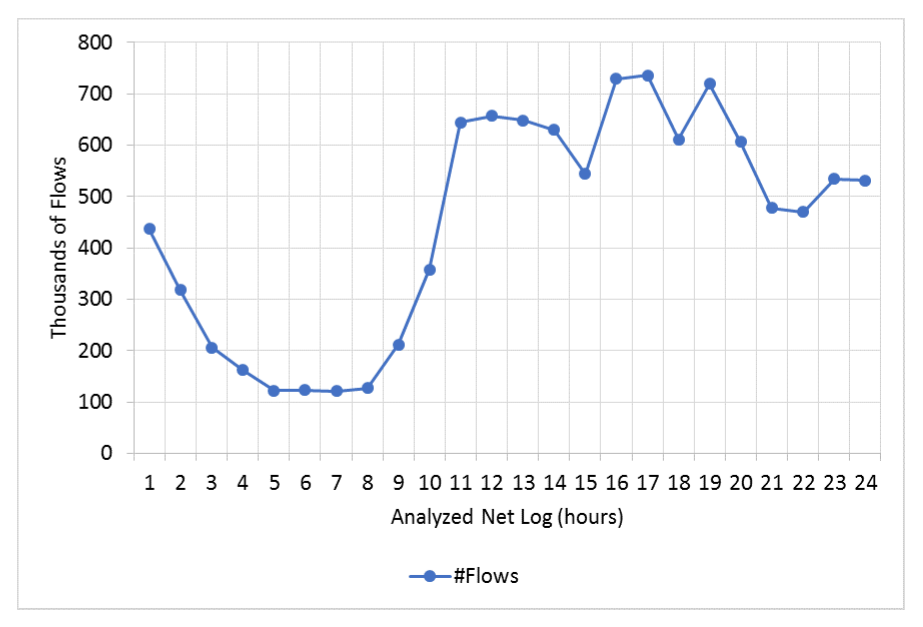
\includegraphics[width=5in]{number_flows.eps}
\caption{Number of flows for each hour of the day.}
\label{number_flows}
\end{figure}

\begin{figure}[!t]
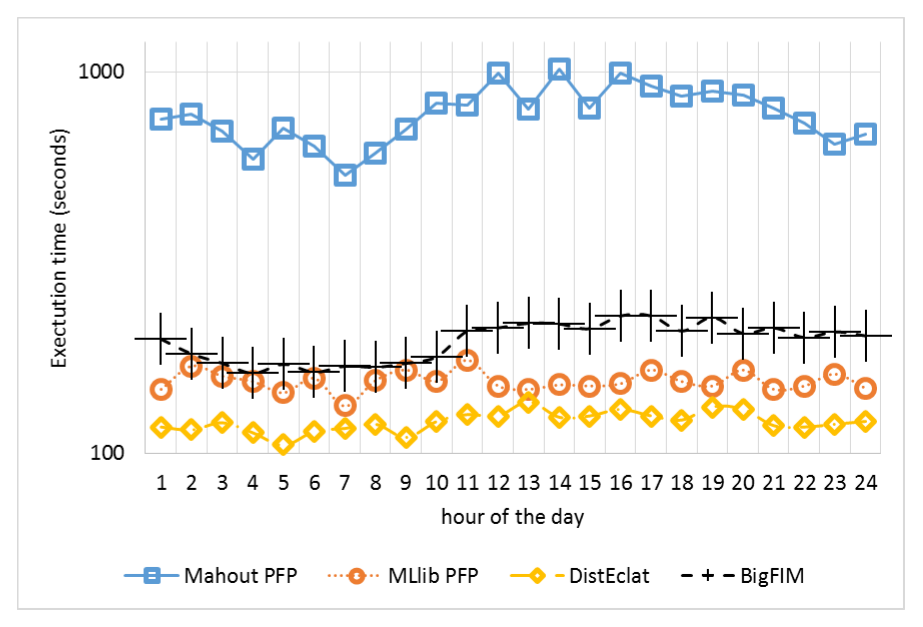
\includegraphics[width=5in]{net_logs_log.eps}
\caption{Execution time of different hours of the day.
(dataset 31, $minsup$=1\%)}
\label{net}
\end{figure}


\begin{table}[h!]
\scriptsize
\begin{center}
\caption{Network traffic flows: number of transactions and frequent itemsets
with $minsup$~0.1\%.}
\label{netlog_itemsets}
\begin{tabular}{|c|c|c|}
\hline
{\bf Hour of}	& {\bf Number of} 	& {\bf	Number of} \\
{\bf the day}	& {\bf transactions} 	& {\bf	frequent itemsets} \\
\hline \hline
0.00  & 437,417 & 166,217 \\ \hline
1.00  & 318,289 & 173,960 \\ \hline
2.00  & 205,930 & 163,266 \\ \hline
3.00  & 162,593 & 166,344 \\ \hline
4.00  & 122,102 & 157,069 \\ \hline
5.00  & 123,683 & 164,493 \\ \hline
6.00  & 121,346 & 170,129 \\ \hline
7.00  & 127,056 & 159,921 \\ \hline
8.00  & 211,641 & 169,751 \\ \hline
9.00  & 357,838 & 187,912 \\ \hline
10.00 & 644,408 & 191,867 \\ \hline
11.00 & 656,965 & 183,021 \\ \hline
12.00 & 648,206 & 184,279 \\ \hline
13.00 & 630,434 & 180,384 \\ \hline
14.00 & 544,572 & 175,252 \\ \hline
15.00 & 729,518 & 192,992 \\ \hline
16.00 & 735,850 & 189,160 \\ \hline
17.00 & 611,582 & 177,808 \\ \hline
18.00 & 719,537 & 179,228 \\ \hline
19.00 & 607,043 & 174,783 \\ \hline
20.00 & 477,760 & 161,153 \\ \hline
21.00 & 470,291 & 159,065 \\ \hline
22.00 & 534,103 & 144,212 \\ \hline
23.00 & 531,276 & 164,516 \\ \hline
\end{tabular}
\end{center}
\end{table}

This use case entails the analysis of a network environment by
using a network traffic log dataset, where each transaction represents a TCP flow.
A network flow is a bidirectional communication between a client and a server.
The dataset has been gathered through Tstat~\cite{Tstat,Tstat2}, a popular
internet traffic sniffer broadly used in
literature~\cite{giordano2015youlighter,ApilettiBCCG13},
by performing a one day capture in three different vantage points
of a nation-wide Internet Service Provider in Italy.
Each transaction of the dataset is associated with
a flow and consists of pairs $(flow~feature, value)$. These features can be
categorical (e.g., TCP Port, Window Scale) or numerical (e.g., RTT,
Number of packets, Number of bytes). Numerical attributes have been discretized by using the same
approach adopted in~\cite{ApilettiBCCG13}.
Finally, we have divided the set of flows (i.e., the set of transactions)
in 1-hour slots, generating 24 sub-datasets.
The number of flows in each sub-dataset
is reported in Figure~\ref{number_flows}.

In this use case, the network administrator is interested in performing hourly
analysis to shape the hourly network traffic.
Hence, we evaluated the performance of the four algorithms,
comparing their execution time, on the 24 hourly sub-datasets.
For all the 24 experiments $minsup$ was set to 1\%, which was
the tradeoff value allowing all the algorithms to complete the extraction.

The results are reported in Figure~\ref{net}, where the performance of the
different approaches show a clear trend: DistEclat always achieves the
lowest execution time, followed by MLlib PFP and BigFIM.
Mahout PFP is the slowest.
The execution time is almost independent of the dataset cardinality,
as it slightly changes throughout the day.
The low dataset size (less than 1~Gigabyte overall)
and cardinality (less than 1~million transactions) make this the ideal
use case for DistEclat, which strongly exploits in-memory computation.



\subsection{Load balancing}
\label{load_exp}


\begin{figure*}[!t]
\begin{center}
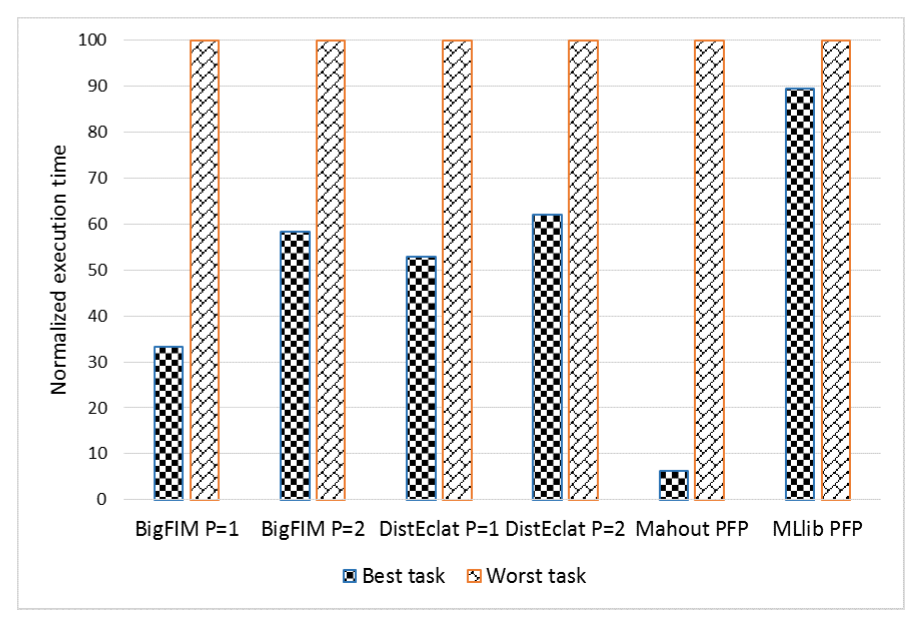
\includegraphics[width=5in]{load_balance_big_2.eps}
\caption{Normalized execution time of the most unbalanced tasks.}
\label{load_balance_big}
\end{center}
\end{figure*}

%\begin{figure*}[!t]
%\begin{center}
%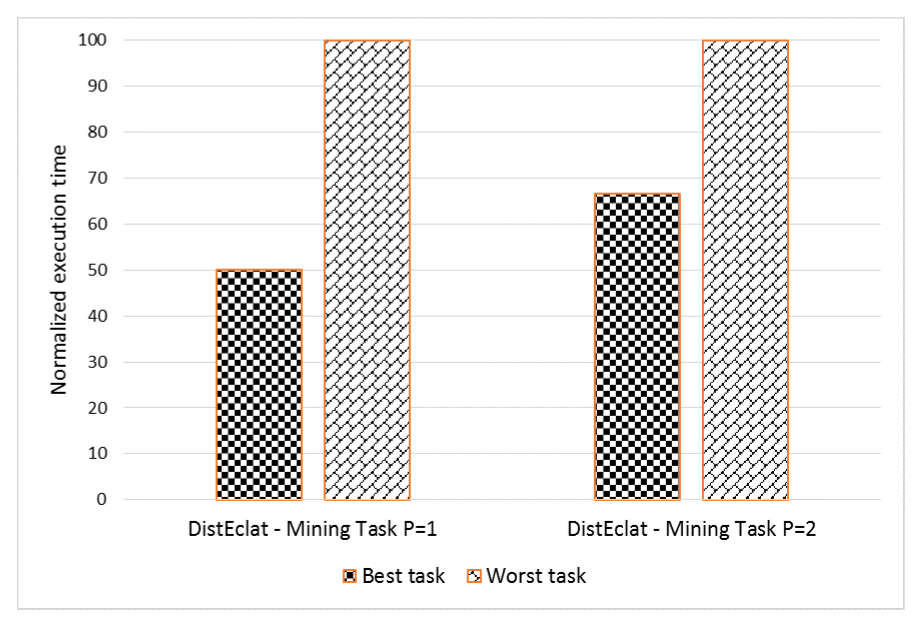
\includegraphics[width=5in]{load_balance_disteclat.eps}
%\caption{Normalized execution time of the most unbalanced tasks of DistEclat.}
%\label{load_balance_disteclat}
%\end{center}
%\end{figure*}

%In this section, experiments address the evaluation of the load balancing
%strategies of the different approaches, an often underestimated issue
%in the distributed data mining bibliography (see Section~\ref{criteria}).
% %The reason is related to the trend to implement in distributed environment
% families of algorithms which were not designed to be distributed.
% %%An example of a bad load balance is what shown in subSection
% ~\ref{attributes_exp} with Mahout PFP: a single task, with an execution period
% more than 30 times higher to the average wallclock time, slows down the whole
% process. On the other hand, approaches such as BigFIM or DistEclat were
% developed taking into account load balance.

We analyzed load balancing on a 1-hour-long subset of the
network log dataset (Table~\ref{datasets_real}) with a fixed $minsup$ of 1\%.
We consider the most unbalanced jobs of each algorithm
and compare the execution times of the fastest and the slowest tasks.
To this aim, we are not interested in the absolute execution time,
but rather in the normalized execution times, where the slowest task is
assigned a value of 100, and the fastest task is compared to such value,
as reported in Figure~\ref{load_balance_big}.

MLlib PFP achieves the best load balancing, with comparable
execution times for all tasks throughout all nodes,
whose difference is in the order of 10\%.
Mahout PFP, instead, shows the worst load balancing issues,
with differences as high as 90\%. The difference between MLlib PFP and Mahout PFP can be correlated to the 
granularity of the subproblems. The smaller the subproblems, the better the load balancing
because their execution times are more similar. MLlib PFP allows specifying the number of partitions, i.e., of subproblems, which obviously impacts on the 
granularity of each subproblem. Hence, setting opportunely this parameter, a good load balancing result is achieved. Differently, 
Mahout PFP automatically sets the number of subproblems and the current heuristic used to set it does not seem to work well on the considered datasets
(unbalanced subproblems are generated).

We included BigFIM and DistEclat with 2 different
first-phase prefix sizes.
For these algorithms, the experiment confirms that a configuration with longer prefixes
leads to a more balanced mining tasks than a configuration with short-sized prefixes,
as mentioned in Subsection~\ref{bigfim}.
%
%For BigFIM, the experiment confirms that a configuration with longer prefixes
%leads to a more balanced mining tasks than a configuration with short-sized prefixes,
%as mentioned in Subsection~\ref{bigfim}.
%Regarding DistEclat, instead, the behavior is the opposite,
%but the values are misleading: considering only the second phase of DistEclat,
%where the trees are mined, as shown in Figure~\ref{load_balance_disteclat},
%the longer the prefixes, the more balanced the mining tasks.
%Hence, DistEclat shows a medium-balanced overall behavior with 1-sized prefixes
%(50\% difference between fastest and slowest tasks),
%a good load balancing for the second phase with 2-sized prefixes (30\% difference),
%and a bad load balancing for the first phase, which affects the overall behavior,
%leading to a final 60\% difference, due to the distribution of the prefixes to
%the different nodes, their expansion and pruning.\\



%\textbf{Discussion:} Given the results of this experiment, the main motivation behind the good performances of BigFIM across all the previous experiments, despite its first phase, is its load balancing, especially with respect to Mahout PFP. As already mentioned, unfortunately, the way used to achieve this good load balancing is critical, because it exposes the algorithm to the cons of an Apriori-like approach (i.e. higher reading and communication costs and weakness with respect to dense problems). 


\subsection{Communication costs}
\label{communication_costs}

\begin{figure*}[!t]
\begin{center}
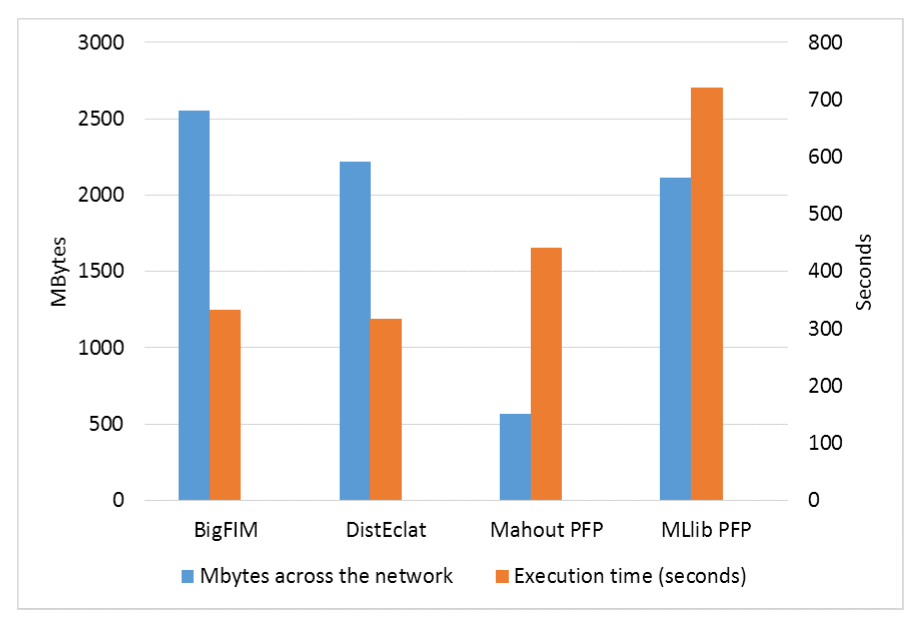
\includegraphics[width=5in]{comm_costs.eps}
\caption{Communication costs and performance for each algorithm,
Datasets~\#1, $minsup$~0.1\%.
The graph reports an average between transmitted and reveiced data.}
\label{comm_costs}
\end{center}
\end{figure*}

%\begin{table*}[h!]
%\begin{center}
%\caption{Execution times for the experiments in Figure~\ref{comm_costs},
%Datasets~\#1, $minsup$~0.1\%.}
%\label{time_comm_costs}
%\begin{tabular}{|c|c|}
%\hline
%{\bf Algorithm }& {\bf Execution time (seconds)}  \\ \hline
% \hline
%BigFIM & 332\\  \hline
%DistEclat &  317 \\ \hline
%Mahout PFP  &442\\ \hline
%MLlib PFP &  614 \\ \hline
%
%\end{tabular}
%\end{center}
%\end{table*}

%\begin{figure*}[!t]
%\begin{center}
%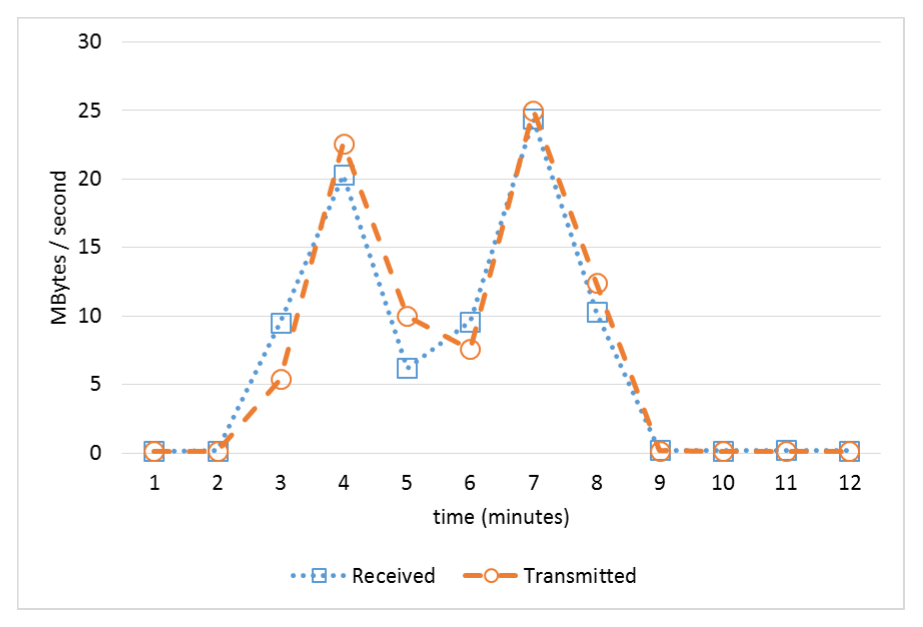
\includegraphics[width=5in]{comm_costs_bigfim.eps}
%\caption{Communication costs of BigFIM, Datasets~\#1, $minsup$~0.1\%.
%The graph reports both transmitted and reveiced data.}
%\label{comm_costs_bigfim}
%\end{center}
%\end{figure*}
%
%\begin{figure*}[!t]
%\begin{center}
%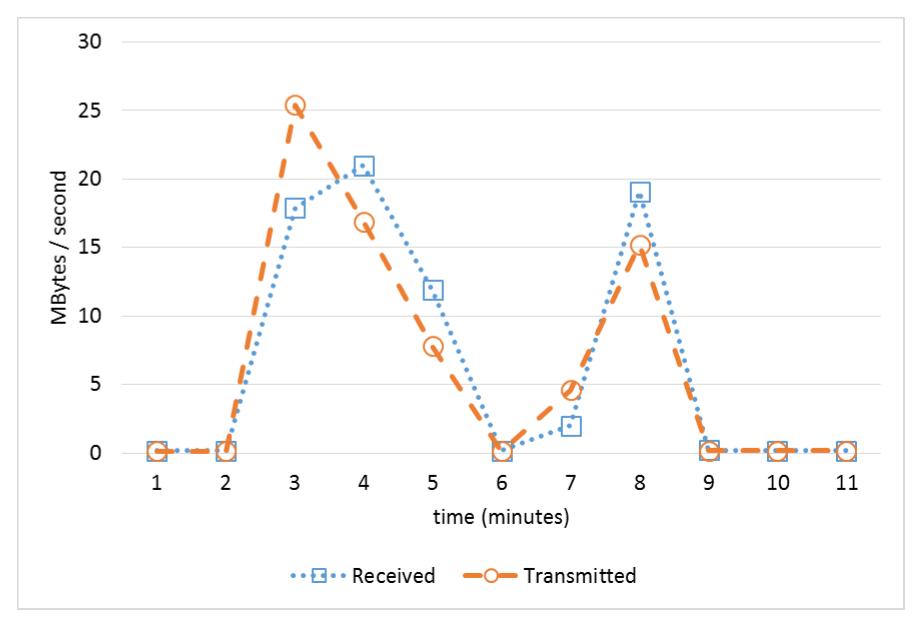
\includegraphics[width=5in]{comm_costs_disteclat.eps}
%\caption{Communication costs of DistEclat, Datasets~\#1, $minsup$~0.1\%.
%The graph reports both transmitted and reveiced data.}
%\label{comm_costs_disteclat}
%\end{center}
%\end{figure*}
%
%\begin{figure*}[!t]
%\begin{center}
%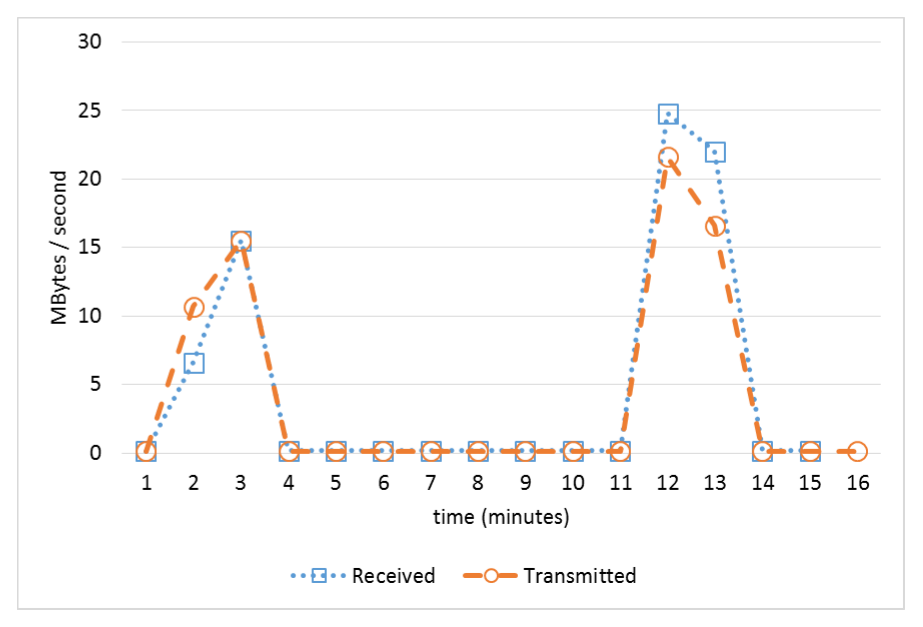
\includegraphics[width=5in]{comm_costs_mllib.eps}
%\caption{Communication costs of MLlib PFP, Datasets~\#1, $minsup$~0.1\%.
%The graph reports both transmitted and reveiced data.}
%\label{comm_costs_mllib}
%\end{center}
%\end{figure*}
%
%\begin{figure*}[!t]
%\begin{center}
%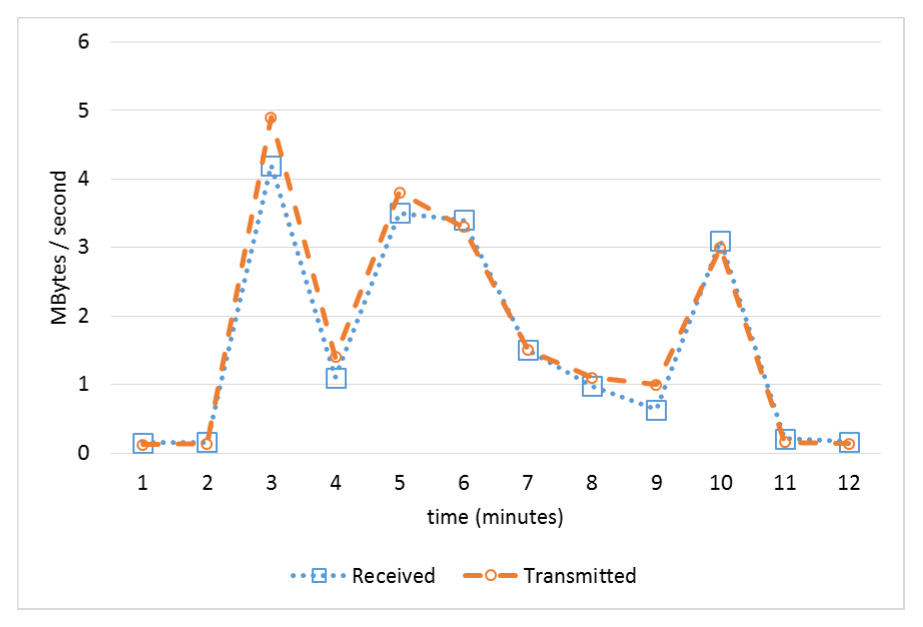
\includegraphics[width=5in]{comm_costs_pfp.eps}
%\caption{Communication costs of Mahout PFP, Datasets~\#1, $minsup$~0.1\%.
%The graph reports both transmitted and reveiced data.
%}
%\label{comm_costs_pfp}
%\end{center}
%\end{figure*}




To evaluate the communication cost, we measure the amount of data transmitted and received
through the nodes network interfaces. This information has been retrieved
by means of the utilities provided by the Cloudera Manager tool.

The experiments have been performed on Dataset~\#1 with a fixed $minsup$ value of 0.1\%,
which was the lowest value for which all algorithms completed the extraction.
Figure~\ref{comm_costs} reports, for each algorithm, the average value
among transmitted and received traffic, compared to the total execution time.
Firstly, the two measures do not seem to be correlated:
higher communication costs are associated with low execution times
for BigFIM and DistEclat, whereas MLlib reports both measures with high values.
Mahout PFP has a communication cost 4 to 5 times lower than all the others,
which exchange an average of 2~Gigabytes of data.
Mahout PFP average communication cost is around 0.5~Gigabytes,
which is approximately the dataset size.
The difference between DistEclat and BigFIM is not large because with only 2-length prefixes just an extra iteration is done by BigFIM.
Even though Mahout PFP is the most communication-cost optimized implementation,
the very low amount of data sent through the network is related
to the adoption of compression techniques, which lead to higher execution times.
%To address this issue,
%we measured the communication costs of the first phase of BigFIM and Mahout PFP
%in word-count toy application. 
%BigFIM generates into the network an
%amount of data more than 5 times larger than Mahout PFP.
%However, at the same time, the execution time of BigFIM initial phase is
%almost 3 times faster than those of Mahout PFP.

%\textbf{Discussion: }These results are consistent with the aformentioned direction. Load Balancing and Communication costs, the main issues in distributed algorithm environment, in this specific scenario do not have the same impact. On the contrary, while the communication costs analysis could be misleading if compared with wall-clock time performances, the behavior of the algorithms in terms of load balancing respect the execution time ranking. We specifically mean MLlib PFP, often the most performant approach, and Mahout PFP, in some experiments unexpectedly outperformed by algorithms theoretically slower. 



\subsection{Discussion}

The experiments confirm that the performance of the data-split-based algorithms
(i.e., BigFIM in its first phase) is highly affected by the number of candidate itemsets, 
which must be stored in the temporary main memory of each task. 
Specifically, BigFIM crashes during its Apriori-based phase when low $minsup$ values or dense datasets are considered,
due to the large number of generated candidate itemsets. 
This issue does not affect the approaches based on the search split strategy (Mahout PFP and MLlib PFP), 
since they do not need to store candidate itemsets as an intermediate result.
Hence, Mahout PFP and MLlib PFP proved to be more suitable than BigFIM to process large dataset sizes, high-density datasets, and low $minsup$ thresholds. 
DistEclat deserves a separate consideration: even if it is based on the search space approach, 
it often runs out of memory,
because in its initial job it needs to store the $tidlists$ of all frequent items in main memory 
and this operation becomes easily unfeasible when large or dense datasets are considered. 
%Hence, DistEclat is exploitable only when relatively small datasets are considered and in that condition it is also the faster algorithm.

Experiments also highlight the predominant importance of load balancing in the itemset mining problem, 
in particular when comparing BigFIM to Mahout PFP. 
Since the initial mining phase of BigFIM is based on the data split parallelization approach,
it reads many times the input dataset (differently than Mahout PFP).
Moreover, BigFIM is also characterized by greater communication costs than Mahout PFP. 
These two factors should impact significantly on the execution time of BigFIM. 
Instead, 
not only the execution time of BigFIM is comparable with that of Mahout PFP 
with 1000-million record datasets (Figure~\ref{transactions}),
but BigFIM is also even faster than Mahout PFP in specific cases, e.g., 
with datasets with an average number of items per transaction greater than 70 (Figure~\ref{attributes}).
The rationale of 	such results is the better load balancing of BigFIM with respect to Mahout PFP. 
Results highlight that load balancing seems to be predominant on the number of dataset reads (I/O costs) and communication costs in the parallelization of the itemset mining problem.





%\textbf{DA RIMUOVERE, confermato (Daniele). Discussion (Versione preparata da Fabio. Da Eliminare una volta verificato che non ci sia qualche parte interessante che non ho riportato nella nuova versione}
%
%In Section~\ref{minsup_exp}, measuring the impact of \textbf{minsup threshold}, we have seen that, as expected, the first phase of BigFIM is fundamental for its scalability. 
%It represents the failure point when the number of candidate itemsets is too large to be stored in the main memory of the mappers. 
%At the same time, thanks to the better load balancing, given by the split of the mining in two balanced phases, BigFIM is able to achieve overall competitive performances (when it does not run out of memory in the first phase). While the failures related to mining tasks characterized by deep search space exploration was expected, because of the weakness of breadth-first approach with respect to data density, for the same reasons, the good performances of BigFIM in terms of execution time were less expected. Probably, the competitive performances were caused by the better load balancing in the search space exploration partitioning.
%
%DistEclat runs easily out of memory because of the size of the input dataset,
%which is transposed in a vertical format during the first phase. 
%The longer tidlists prevent it from completing such step. Even for this algorithm, the first phase is critical. The assumption of storing almost all the input dataset in all the nodes, at the aim of saving reading phases and communication costs, revealed to be not suitable for a problem characterized by a deep search space exploration.
%
%Mahout PFP and MLlib PFP are the only algorithms
%to complete the mining tasks for all $minsup$ values.
%Precisely, Mahout PFP is the most suitable technique
%when dealing with minsup values over 0.05\%,
%with a performance 6 to 8 times faster than the MLlib sibling.
%However, with lower $minsup$ values,
%Spark MLlib becomes the fastest approach with an order of magnitude gap.
%We identified the cause of the different performance
%between the two PFP implementations
%in the different pruning strategies.
%The algorithms which extract closed itemsets, such as Mahout PFP,
%can apply more effective pruning techniques
%that are not applicable when all frequent itemsets must be extracted,
%which is the case for MLlib PFP.
%When the problem becomes deeper and more challenging, beyond the engineering differences between the two implementations, the better load balancing of the MLlib PFP makes it faster.
%
%In Section~\ref{attributes_exp}, instead, we have measured the impact of \textbf{the length of the transactions} on the mining performances. As expected (see Figure~\ref{attributes_deeper}), for more dense data distributions the number of candidate itemsets increases and BigFIM runs out of memory due to its initial Apriori phase. 
%A similar motivation holds for DistEclat failures, due to its requirement to store all the (longer) tidlists in all the nodes.
%The FP-growth based approaches are affected by the increasing length of the transactions. However, their depth-first structure revealed to be the best exploration strategy in such an environment (i.e. high number of attributes). 
%DistEclat leverages a depth-first exploration strategy as well, however it assumes that all the tidlists should be stored in all the commodity cluster nodes, which is challenging if considering the further memory requirements due to the search space exploration. 
%
%In Section~\ref{nr_machines} the \textbf{speedup} achieved by the algorithms with different \textbf{degrees of parallelization} is evaluated. Based on the results it is clear that many of the considered algorithms are not able to properly exploit the parallelism provided by distributed frameworks. The reason 
%is probably given by the fact that they are not able to split the initial problem in a number of subproblems equal to the number of available parallel 
%tasks, or, when they are able to do so, the overhead given by the instance of the subtasks is greater than the advantages given by the parallel execution 
%of the subtasks/subproblems.
%
%\textbf{Load balance}, one the most important distributed features, is evaluated in Section~\ref{load_exp}.
% Given the results of this experiment, the main motivation behind the good performances of BigFIM across all the previous experiments, despite its first phase, is its load balancing, especially with respect to Mahout PFP. 
%As already mentioned, unfortunately, the way used to achieve this good load balancing is critical, because it exposes the algorithm to the cons of an Apriori-like approach (i.e. higher reading and communication costs and weakness with respect to dense problems). 
%
%Finally, Section~\ref{communication_costs}, analyzes the \textbf{communications costs} related to the mining, in terms of data transmitted in the commodity cluster network. These results suggest that Load Balancing and Communication costs, the main issues in distributed algorithm environment, in this specific scenario do not have the same impact. On the contrary, while the communication costs analysis could be misleading if compared with wall-clock time performances, the behavior of the algorithms in terms of load balancing respects the execution time ranking. For instance, Mahout PFP, in some experiments is unexpectedly outperformed by algorithms with higher communication costs. 
%
%

%\textbf{Discussion (Fabio: Recap di tutte le discussion precedenti che sono state commentate)}
%
%In Section~\ref{minsup_exp}, measuring the impact of \textbf{minsup threshold}, we have seen that, as expected, the first phase of BigFIM is fundamental for its scalability. 
%It represents the failure point when the number of candidate itemsets is too large to be stored in the main memory of the mappers. 
%At the same time, thanks to the better load balancing, given by the split of the mining in two balanced phases, BigFIM is able to achieve overall competitive performances (when it does not run out of memory in the first phase). While the failures related to mining tasks characterized by deep search space exploration was expected, because of the weakness of breadth-first approach with respect to data density, for the same reasons, the good performances of BigFIM in terms of execution time were less expected. Probably, the competitive performances were caused by the better load balancing in the search space exploration partitioning.
%
%DistEclat runs easily out of memory because of the size of the input dataset,
%which is transposed in a vertical format during the first phase. 
%The longer tidlists prevent it from completing such step. Even for this algorithm, the first phase is critical. The assumption of storing almost all the input dataset in all the nodes, at the aim of saving reading phases and communication costs, revealed to be not suitable for a problem characterized by a deep search space exploration.
%
%Mahout PFP and MLlib PFP are the only algorithms
%to complete the mining tasks for all $minsup$ values.
%Precisely, Mahout PFP is the most suitable technique
%when dealing with minsup values over 0.05\%,
%with a performance 6 to 8 times faster than the MLlib sibling.
%However, with lower $minsup$ values,
%Spark MLlib becomes the fastest approach with an order of magnitude gap.
%We identified the cause of the different performance
%between the two PFP implementations
%in the different pruning strategies.
%The algorithms which extract closed itemsets, such as Mahout PFP,
%can apply more effective pruning techniques
%that are not applicable when all frequent itemsets must be extracted,
%which is the case for MLlib PFP.
%When the problem becomes deeper and more challenging, beyond the engineering differences between the two implementations, the better load balancing of the MLlib PFP makes it faster.
%
%In Section~\ref{attributes_exp}, instead, we have measured the impact of \textbf{the length of the transactions} on the mining performances. As expected (see Figure~\ref{attributes_deeper}), for more dense data distributions the number of candidate itemsets increases and BigFIM runs out of memory due to its initial Apriori phase. 
%A similar motivation holds for DistEclat failures, due to its requirement to store all the (longer) tidlists in all the nodes.
%The FP-growth based approaches are affected by the increasing length of the transactions. However, their depth-first structure revealed to be the best exploration strategy in such an environment (i.e. high number of attributes). 
%DistEclat leverages a depth-first exploration strategy as well, however it assumes that all the tidlists should be stored in all the commodity cluster nodes, which is challenging if considering the further memory requirements due to the search space exploration. 
%
%In Section~\ref{nr_machines} the \textbf{speedup} achieved by the algorithms with different \textbf{degrees of parallelization} is evaluated. Based on the results it is clear that many of the considered algorithms are not able to properly exploit the parallelism provided by distributed frameworks. The reason 
%is probably given by the fact that they are not able to split the initial problem in a number of subproblems equal to the number of available parallel 
%tasks, or, when they are able to do so, the overhead given by the instance of the subtasks is greater than the advantages given by the parallel execution 
%of the subtasks/subproblems.
%
%\textbf{Load balance}, one the most important distributed features, is evaluated in Section~\ref{load_exp}.
% Given the results of this experiment, the main motivation behind the good performances of BigFIM across all the previous experiments, despite its first phase, is its load balancing, especially with respect to Mahout PFP. 
%As already mentioned, unfortunately, the way used to achieve this good load balancing is critical, because it exposes the algorithm to the cons of an Apriori-like approach (i.e. higher reading and communication costs and weakness with respect to dense problems). 
%
%Finally, Section~\ref{communication_costs}, analyzes the \textbf{communications costs} related to the mining, in terms of data transmitted in the commodity cluster network. These results suggest that Load Balancing and Communication costs, the main issues in distributed algorithm environment, in this specific scenario do not have the same impact. On the contrary, while the communication costs analysis could be misleading if compared with wall-clock time performances, the behavior of the algorithms in terms of load balancing respects the execution time ranking. For instance, Mahout PFP, in some experiments is unexpectedly outperformed by algorithms with higher communication costs. 
%




%%\\
%\textbf{fabio: eliminerei da qui in poi}
%Investigating deeper into the specific algorithm communication-cost analisys,
%Figures~\ref{comm_costs_bigfim},~\ref{comm_costs_disteclat},~\ref{comm_costs_mllib},~\ref{comm_costs_pfp}
%show the data exchanged throughout the whole execution time
%of each algorithm.
%
%BigFIM and DistEclat, in
%Figure~\ref{comm_costs_bigfim},~\ref{comm_costs_disteclat}, have a similar
%behaviour, with the communication costs grouped into two main phases.
%The first phase is related to the prefix extraction,
%while the second one matches the prefix preparation and prefix tree mining.
%BigFIM saturates the network link capacity (25~Megabytes/s, corresponding to
%a 100~Mbit/s full duplex Ethernet interface) during the second phase peak
%at minute 7 for both sent and received data,
%whereas DistEclat reaches such point during the first phase at minute 3,
%in trasmitted data only.
%BigFIM is also continuously exchanging data through the network during the
%mining process, whereas DistEclat pauses the network data exchange at minute 6.
%% %The choice of doing the main tasks of each job (prefix mining and prefix
%% expansion) in the map phase, without a full exploitation of data locality,
%% strongly affects communication costs. On the other hand, for instance, Mahout
%% PFP first phase, in which the header table is obtained through a basic
%% WordCount, each mapper exploits data locality working on its shard of the
%% dataset.
%Also the MLlib PFP implementation (Figure~\ref{comm_costs_mllib})
%presents two phases: differently from BigFIM and DistEclat, the middle ``pause'',
%dividing the first shuffling phase and the second materialization phase,
%is very long and lasts from minute 4 to minute 11,
%it is immediately followed by a peak reaching the network capacity
%at minute 12.
%Mahout PFP communication costs, instead, (Figure~\ref{comm_costs_pfp})
%consists of three phases:
%the first is related to the counting part,
%the second one corresponds to the mining phase,
%while the last one is related to the aggregation of the results.
%The peak in network data exchange is as low as 5~Mbytes/s.
%
%
%
%%
%% %However, interestingly, the behaviour does not affect the execution time of
%% this mining experiment, in which the considered implementation is outperformed
%% by BigFIM and DistEclat as shown in Table~\ref{time_comm_costs}. The reason is
%% partially related to an unfair load balancing, sinche the longest mining task
%% lasts more than three times the execution time of the fastest ones.
%
%
%%
%%
%%\section{Lessons learned FABIO: LE  METTEREI DOPO LE OPEN ISSUES}
%%\label{lesson}
%%
%%\textbf{Da Modificare: - modificare alcuni risultati legati a bigfim;  - aggiungere per il secondo reviewer le istruzioni su quanto sia facile utilizzarli; -esplicitare meglio i failures scenario visto che li ha richiesti}
%%
%%The reported experiments provide a wide view of the different behaviours of the
%%algorithms, dealing with diverse types of problems.
%%With this section, we aim at supporting the reader
%%in a conscious choice of the most suitable approach,
%%depending on the use case at hand.
%%Pursuing this target, we measured the real-life performance
%%of the openly-available frequent-pattern mining implementations
%%for the most popular distributed platforms (i.e., Hadoop and Spark).
%%They have been tested on many different datasets
%%characterised by different values of
%%minimum support ($minsup$),
%%transaction length (dimensionality),
%%number of transactions (cardinality),
%%and dataset density,
%%besides two real-life use cases.
%%Perfomance in terms of execution time, load balancing, and communication cost
%%have been evaluated:
%%a one-table summary of the results is reported in Table~\ref{all_resume}.
%%As a result of the described experience,
%%the following general suggestions emerge:
%%
%%\begin{itemize}
%% \item
%% Without prior knowledge of dataset density, dimensionality
%% (average transaction length), and cardinality (number of transactions),
%% \textbf{Mahout PFP} is the algorithm that best guarantees
%% the mining task completion,
%% at the expense of longer execution times.
%% Mahout PFP is the only algorithm able to always reach the experimental limits.
%% Furthermore, it exchanges very few data across the network of the cluster.
%% \item
%% When the dataset size is small with respect to the available memory,
%% \textbf{DistEclat} has proven to be among the fastest approaches,
%% and also to be able to reach the lowest experimental $minsup$ values.
%% DistEclat experiments showed that it cannot scale for large or
%% high-dimensional datasets, but when it can complete the itemset extraction,
%% it is very fast.
%% \item
%% On most real-world use cases, with limited dimensionality
%% (up to 60 items per transaction on average), \textbf{MLlib PFP}
%% has proven to be the most reasonable tradeoff choice,
%% with fast execution times and optimal scalability to very large datasets.
%% \item
%% Finally, for high-dimensional datasets, \textbf{BigFIM} resulted
%% the fastest approach,
%% but it cannot cope with $minsup$ values as low as the others.
%%\end{itemize}
%%
%%\begin{table*}[h!]
%%\scriptsize
%%\begin{center}
%%\caption{
%%Summary of the limits identified by the experimental evaluation of the
%%algorithms (lowest $minsup$, maximum transaction length,
%%largest dataset cardinality).
%%The faster algorithm for each experiment is marked in bold.
%%}
%%\label{all_resume}
%%\begin{tabular}{|c|c|c|c|c|}
%%\hline
%%& Section \ref{minsup_exp} & Section \ref{minsup_exp} & Section \ref{attributes_exp}& Section  \ref{transaction_exp} \\ \hline
%%% & Transaction & Transaction& Minsup value: 1\% & Minsup value 0.4 \% \\
%%% &  length: 10 & length: 30 &  &  \\ \hline
%%% & 10M transactions & 10M transactions &  10M transactions &  Transaction length 10 \\ \hline
%%% & Dataset \#1 & Dataset &  Dataset &  Dataset \\ \hline
%%           & $minsup$ & $minsup$ & transaction  & millions of   \\
%%           &          &          & length       & transactions  \\ \hline
%%Mahout PFP & 0.002\% & 0.01\%    & 100          & 100 		\\ \hline
%%MLlib PFP  & 0.002\% & \textbf{0.01\%}   & 60		& \textbf{100} 	\\ \hline
%%BigFIM     & 0.1\%   & 0.3\%     & \textbf{100} 	& 100 		\\ \hline
%%DistEclat  & \textbf{0.002\%}& - 	 & - 		& 1 		\\ \hline
%%\end{tabular}
%%\end{center}
%%\end{table*}
%%
%%%\begin{table*}[h!]
%%%\begin{center}
%%%\caption{Experimental result summary.
%%%\textbf{@FABIO8: qui secondo me devi fare una colonna per ogni subsection sperimentale,
%%%es. colonna ``valore minimo di $minsup$, Section X.Y'' e riporti i valori limite,
%%%ecc. con le altre subsection... cos\`i invece non mi piace, non \`e immediato
%%%da capire... e poi magari metterei un asterisco sul metodo pi\`u veloce
%%%(o i due pi\`u veloci se sono molto simili) in ogni colonna.
%%%Se non \`e chiaro ci sentiamo.}
%%%}
%%%\label{all_resume}
%%%\begin{tabular}{|c|c|c|c|c|}
%%%\hline
%%%           & Transaction & Transaction& Minsup value: 1\% & Minsup value 0.4 \% \\
%%%  &  length: 10 & length: 30 &  &  \\ \hline
%%%            & 10M transactions & 10M transactions &  10M transactions &  Transaction length 10 \\ \hline
%%%Algorithm  & Lowest minsup:                           & Lowest minsup:                             & Max. transaction           & Max. number of   \\
%%%  &                       &                             &  length:           & transactions (millions):   \\ \hline
%%%Mahout PFP & 0.002 \%                                  & 0.01 \%                                   & 100                                  & 100                                         \\ \hline
%%%MLlib PFP  & 0.002 \%                                  & 0.01 \%                                   & 60                                   & 100                                         \\ \hline
%%%BigFIM     & 0.1 \%                                    & 0.3 \%                                    & 100                                  & 100                                         \\ \hline
%%%DistEclat  & 0.002 \%                                  & -                                         & -                                    & 1                                           \\ \hline
%%%\end{tabular}
%%%\end{center}
%%%\end{table*}
%
%
%
%

\section{Lessons Learned}
\label{lesson}


The reported experiments provide a wide view of the different behaviours of the
algorithms in various experimental settings.
With this section, we aim at supporting the reader
in a conscious choice of the most suitable approach,
depending on the use case at hand.
Pursuing this target, we measured the real-life performance
of the openly-available frequent-pattern mining implementations
for the most popular distributed platforms (i.e., Hadoop and Spark).
They have been tested on many different datasets
characterized by different values of
minimum support ($minsup$),
transaction length (dimensionality),
number of transactions (cardinality),
and dataset density,
besides two real-life use cases.
Performance in terms of execution time, load balancing, and communication cost
have been evaluated:
a one-table summary of the results is reported in Table~\ref{all_resume}.
As a result of the described experience,
the following general suggestions emerge:

\begin{itemize}
 \item {\bf High reliability.}
 Without prior knowledge of dataset density, dimensionality
 (average transaction length), and cardinality (number of transactions),
 \textbf{Mahout PFP} is the algorithm that best guarantees
 the mining task completion,
 at the expense of longer execution times.
 Mahout PFP is the only algorithm able to always reach the experimental limits.


 \item {\bf High cardinality and low-dimensional data.}
 On most real-world use cases, with limited dimensionality
 (up to 60 items per transaction on average), \textbf{MLlib PFP}
 has proven to be the most reasonable tradeoff choice,
 with fast execution times and optimal scalability to very large datasets.

 \item {\bf High-dimensional data.}
 For high-dimensional datasets, \textbf{BigFIM} resulted
 the fastest approach, but it cannot cope with $minsup$ values as low as the others. In those cases, \textbf{Mahout PFP} represents the only option.

 \item {\bf Limited dataset size.}
 When the dataset size is small with respect to the available memory,
 \textbf{DistEclat} has proven to be among the fastest approaches,
 and also to be able to reach the lowest experimental $minsup$ values.
 DistEclat experiments showed that it cannot scale for large or
 high-dimensional datasets, but when it can complete the itemset extraction,
 it is very fast.

\end{itemize}

%From an even more practical point of view, all the implementations revealed to be quite easy to deploy and use. 
%Actually, the only requirement for all the implementations to be run was the Hadoop/Spark installation 
%(from a single machine scenario to a large cluster). 
%Only the MLlib PFP implementation requires few additional steps, since it is delivered as a library requiring some coding skills: 
%the users should develop their own class and compile it.

\begin{table*}[h!]
\scriptsize
\begin{center}
\caption{
Summary of the limits identified by the experimental evaluation of the
algorithms (lowest $minsup$, maximum transaction length,
largest dataset cardinality).
The faster algorithm for each experiment is marked in bold.
}
\label{all_resume}
\begin{tabular}{|c|c|c|c|c|}
\hline
& Section \ref{minsup_exp} & Section \ref{minsup_exp} & Section \ref{attributes_exp}& Section  \ref{transaction_exp} \\ \hline
% & Transaction & Transaction& Minsup value: 1\% & Minsup value 0.4 \% \\
% &  length: 10 & length: 30 &  &  \\ \hline
% & 10M transactions & 10M transactions &  10M transactions &  Transaction length 10 \\ \hline
% & Dataset \#1 & Dataset &  Dataset &  Dataset \\ \hline
           & $minsup$ & $minsup$ & transaction  & millions of   \\
           &          &          & length       & transactions  \\ \hline
Mahout PFP & 0.002\% & 0.01\%    & \textbf{100 (0.1\%)}          & 100 		\\ \hline
MLlib PFP  & 0.002\% & \textbf{0.01\%}   & 60		& \textbf{100} 	\\ \hline
BigFIM     & 0.1\%   & 0.3\%     & 100 (1\%) 	& 100 		\\ \hline
DistEclat  & \textbf{0.002\%}& - 	 & - 		& 1 		\\ \hline
\end{tabular}
\end{center}
\end{table*}

%\begin{table*}[h!]
%\begin{center}
%\caption{Experimental result summary.
%\textbf{@FABIO8: qui secondo me devi fare una colonna per ogni subsection sperimentale,
%es. colonna ``valore minimo di $minsup$, Section X.Y'' e riporti i valori limite,
%ecc. con le altre subsection... cos\`i invece non mi piace, non \`e immediato
%da capire... e poi magari metterei un asterisco sul metodo pi\`u veloce
%(o i due pi\`u veloci se sono molto simili) in ogni colonna.
%Se non \`e chiaro ci sentiamo.}
%}
%\label{all_resume}
%\begin{tabular}{|c|c|c|c|c|}
%\hline
%           & Transaction & Transaction& Minsup value: 1\% & Minsup value 0.4 \% \\
%  &  length: 10 & length: 30 &  &  \\ \hline
%            & 10M transactions & 10M transactions &  10M transactions &  Transaction length 10 \\ \hline
%Algorithm  & Lowest minsup:                           & Lowest minsup:                             & Max. transaction           & Max. number of   \\
%  &                       &                             &  length:           & transactions (millions):   \\ \hline
%Mahout PFP & 0.002 \%                                  & 0.01 \%                                   & 100                                  & 100                                         \\ \hline
%MLlib PFP  & 0.002 \%                                  & 0.01 \%                                   & 60                                   & 100                                         \\ \hline
%BigFIM     & 0.1 \%                                    & 0.3 \%                                    & 100                                  & 100                                         \\ \hline
%DistEclat  & 0.002 \%                                  & -                                         & -                                    & 1                                           \\ \hline
%\end{tabular}
%\end{center}
%\end{table*}






\section{Open research issues}
\label{openissues}
%
Following the analysis of the state-of-the-art in frequent itemset mining
algorithms for distributed computing frameworks, and the in-depth experimental
evaluation discussed in Section~\ref{experimental},
we can deduce that different efficient and scalable
algorithms have been designed and developed during the last years.
However, despite the technological advancements, there is still room for
improvements. Specifically,
some open problems, summarized below, should be addressed to support
a more effective and efficient data mining process on Big Data collections.

\textbf{Algorithm selection.}
Many algorithms have been proposed in literature
to efficiently extract correlations among data in the form of frequent itemsets,
as discussed in this review.
However, to apply one of the above algorithms for the analysis of a given
dataset, the analyst needs to identify
the best algorithm suitable for her use case,
able to efficiently deal with the
underlying data characteristics.
The selection process is mainly based on the analyst expertise and must be
handpicked for a given dataset.
Thus, innovative and effective techniques that can intelligently and
automatically support the analyst in the identification of the best algorithm
for the current use case analysis are needed.

\textbf{Parameter setting.}
The performance of the available algorithms to extract frequent
itemsets depends on the choice of the input parameters, like the support
threshold, which dramatically impacts the execution time based on the data
distribution characteristics. The optimal trade-off between execution time and
result accuracy must be manually selected for any given application, based on
the
analysts expertise.
To extract meaningful and interesting itemsets while maintaining the
number of extracted results within manageable limits, a large number of
experiments should be performed and the results
manually evaluated by domain experts.
The whole process is time consuming and requires a considerable
amount of effort and skills. Thus, new scalable approaches
capable of self-configuring to automatically extract actionable
knowledge from massive data repositories
are needed.

\textbf{Missing support for really high-dimensional datasets}
The performance analysis have included a mining experiments on datasets with 
up to 100 dimensions. Even if BigFIM has outperformed the competitors, its performances
are still very weak for low minimum support values. On the other hand, 100-features dataset certainly
do not represent a state-of-the-art high dimensional problem, which can be instead characterized by thousands of million of dimensions.
Thus, arises from the review is a concrete lack of a real scalable implementation which focus on the number of
items per transaction. 

\textbf{Full exploitation of computational capabilities of distributed
frameworks.}
Up to now, data mining algorithms have been mainly designed to be
optimized when running on centralized architectures.
Furthermore, recursive primitives cannot be easily translated into
distributed approaches,
thus the efficiency of the current distributed
implementations are limited.
There is room for novel approaches natively
designed to be distributed, able to efficiently address the itemset
mining discovery and to fully exploit computational capabilities of
distributed frameworks.




%Following the analysis of the state-of-the-art in frequent itemset mining
%algorithms for distributed computing frameworks, and the in-depth experimental
%evaluation discussed in Section~\ref{experimental},
%we can deduce that different efficient and scalable
%algorithms have been designed and developed during the last years.
%The review followed a structured analysis. After a theoretical description of the algorithmic design choices
%in terms of exploration and distribution of the search space, we introduced two aspects more related to distributed environment, such as Load Balancing and Communication costs. After this initial theoretical phase, we have largely put to the test all the algorithms in several possible use cases, leveraging both synthetic and real datasets. Indeed, the experiments results, in some cases, did not achieve the expectations related to theoretical analysis. These events allowed us to better understand  the impact of the aforementioned aspects on the final performances and, in general, on distributed frequent itemset mining domain.

%This type of analysis, which is, to our knowledge, unique in the state of the art, allowed us to extract very interesting take-aways and open questions. 

The comparative study presented in this review highlighted interesting research directions to enhance distributed itemset mining algorithms for Big Data.


\textbf{Smarter load balancing techniques.} 
The experimental evaluation allowed us to show that load balancing issues significantly affect distributed itemset mining performance, more than communication and I/O costs (e.g., reading the dataset many times). 
Specifically, the different complexity among the task-level sub-problems leads to load unbalance in the cluster 
(i.e., some sub-problems are more computationally expensive and time consuming than others causing inefficient resource usage).
%the largest sub-problems could be still too complex to be analyzed in a single task causing worse performance or the bottleneck in memory allocation).
Load balancing improvements should be addressed in the design of new distributed frequent itemset mining algorithms. 
In that context, we believe that a new research direction to investigate is the definition of variable-length prefixes, 
with respect to which the mining sub-problems are defined, 
hence leading to a more balanced exploration of the search space. 

%\textbf{Innovative scheduling schema.} 
%{\bf Paolo. Ci\`o che \`e descritto dopo non mi sembra sia un problema di scheduling. Non mi torna. Da discutere.}
%{\bf Paolo. Questa parte va rivista in base a come Elena sta modificando le lettere. Sar\`a molto piu smorzato nelle lettere e quindi bisogna capire come cambiare questo punto.}
%The experiments highlighted the unreliability of approaches optimizing reading phases and communications cost in the sake of performance. In the frequent itemset mining domain, the input datasets are often much smaller than the data structures the algorithms should keep in memory. Given this peculiarity, reading costs hardly dominate the overall performance. 
%The reduction of the communication costs should be addressed in the design of innovative scheduling schema to give a higher priority to appropriate tasks 
%\textbf{PER FABIO: NON HO CAPITO cosa volevate dire. RIESCI A FINIRE LA FRASE?}
%\textbf{Fabio: Non sono d'accordo sull'evoluzione di questo paragrafo. Non so se l'hai trovato già così ma secondo me lo scheduling centra poco. La versione che avevo scritto io forse è troppo prolissa. Forse la versione di Elena nella lettera è equilibrata.. te la cito: the experiments highlighted the unreliability of approaches optimizing reading phases and communications cost in the sake of performance. In the frequent itemset mining domain, the input datasets are often much smaller than the data structures the algorithms should keep in memory. Given this peculiarity, reading costs hardly dominate the overall performance. Hence, a higher priority should be given to an appropriate and balanced handling of the inner structures exploited for the itemsets extraction. }



%However, despite the technological advancements, there is still room for
%improvements. Specifically,
%some open problems, summarized below, should be addressed to support
%a more effective and efficient data mining process on Big Data collections.



\textbf{Self-tuning itemset mining frameworks.} 
As discussed in the paper, different algorithms have been proposed in literature
to discover frequent itemsets. 
However, the efficient exploitation of each algorithm strongly depends on specific skills and expertise. 
The analyst is required to select the best method to efficiently deal with the
underlying data characteristics, 
and manually configure it 
(e.g., from input parameters settings, such as the $minsup$ threshold, the $k$ parameter of BigFIM, etc., to distributed frameworks tuning).
%The optimal trade-off between execution time and
%result accuracy {\bf Paolo. Cos'è l'accuracy per gli itemset?} must be manually selected for any given application, based on
%the analysts expertise.
Thus, state-of-the-art algorithms may become ineffective because of the inefficient hand-picked choices 
of the inappropriate specific implementations, and cumbersome parameter-configuration sessions.
The improvements in algorithm usability should be addressed by designing innovative self-tuning itemset mining 
frameworks, capable of intelligently selecting the most appropriate itemset extraction algorithm 
and automatically configuring it.



% \textbf{Full exploitation of computational capabilities of distributed frameworks.}
% Up to now, data mining algorithms have been mainly designed to be optimized when running on centralized architectures.
% Furthermore, recursive primitives cannot be easily translated into distributed approaches,
% thus the efficiency of the current distributed implementations are limited.
% There is room for novel approaches natively designed to be distributed, able to efficiently address the itemset
% mining discovery and to fully exploit computational capabilities of distributed frameworks.


\section*{Acknowledgement}
The research leading to these results has received funding from the European
Union under the FP7 Grant Agreement n. 619633 (Project ``ONTIC'').

%% The Appendices part is started with the command \appendix;
%% appendix sections are then done as normal sections
%% \appendix

%% \section{}
%% \label{}

%% If you have bibdatabase file and want bibtex to generate the
%% bibitems, please use
%%
%\bibliographystyle{elsarticle-num}
%\bibliography{biblio}{}
\begin{thebibliography}{10}
\expandafter\ifx\csname url\endcsname\relax
  \def\url#1{\texttt{#1}}\fi
\expandafter\ifx\csname urlprefix\endcsname\relax\def\urlprefix{URL }\fi
\expandafter\ifx\csname href\endcsname\relax
  \def\href#1#2{#2} \def\path#1{#1}\fi

\bibitem{DBLP:journals/bdr/Al-JarrahYMKT15}
O.~Y. Al{-}Jarrah, P.~D. Yoo, S.~Muhaidat, G.~K. Karagiannidis, K.~Taha,
  Efficient machine learning for big data: {A} review, Big Data Research 2~(3)
  (2015) 87--93.

\bibitem{Xu_2005SurveyClustering}
R.~Xu, D.~Wunsch, II, Survey of clustering algorithms, Trans. Neur. Netw.
  16~(3) (2005) 645--678.

\bibitem{Han_2007SurveyFIM}
J.~Han, H.~Cheng, D.~Xin, X.~Yan, Frequent pattern mining: Current status and
  future directions, Data Min. Knowl. Discov. 15~(1) (2007) 55--86.

\bibitem{AggarwalBookClassification}
C.~C. Aggarwal, Data Classification: Algorithms and Applications, 1st Edition,
  Chapman \& Hall/CRC, 2014.

\bibitem{HDFS}
D.~Borthakur, The hadoop distributed file system: Architecture and design,
  Hadoop Project 11 (2007) 21.

\bibitem{Zaharia_spark}
M.~Zaharia, M.~Chowdhury, T.~Das, A.~Dave, J.~Ma, M.~McCauley, M.~J. Franklin,
  S.~Shenker, I.~Stoica, Resilient distributed datasets: A fault-tolerant
  abstraction for in-memory cluster computing, in: NSDI'12, 2012, pp. 2--2.

\bibitem{ApilettiBCCG13}
D.~Apiletti, E.~Baralis, T.~Cerquitelli, S.~Chiusano, L.~Grimaudo, Searum: {A}
  cloud-based service for association rule mining, in: 12th {IEEE}
  International Conference on Trust, Security and Privacy in Computing and
  Communications, TrustCom 2013 / 11th {IEEE} International Symposium on
  Parallel and Distributed Processing with Applications, {ISPA-13} / 12th
  {IEEE} International Conference on Ubiquitous Computing and Communications,
  IUCC-2013, Melbourne, Australia, July 16-18, 2013, 2013, pp. 1283--1290.

\bibitem{META-TIST-2015}
D.~Antonelli, E.~Baralis, G.~Bruno, L.~Cagliero, T.~Cerquitelli, S.~Chiusano,
  P.~Garza, N.~A. Mahoto, {MeTA: Characterization of Medical Treatments at
  Different Abstraction Levels}, {ACM} {TIST} 6~(4) (2015) 57.

\bibitem{DBLP:conf/sigmod/CongXPTY04}
G.~Cong, A.~K.~H. Tung, X.~Xu, F.~Pan, J.~Yang,
  \href{http://doi.acm.org/10.1145/1007568.1007587}{{FARMER:} finding
  interesting rule groups in microarray datasets}, in: G.~Weikum, A.~C.
  K{\"{o}}nig, S.~De{\ss}loch (Eds.), Proceedings of the {ACM} {SIGMOD}
  International Conference on Management of Data, Paris, France, June 13-18,
  2004, {ACM}, 2004, pp. 143--154.
\newblock \href {http://dx.doi.org/10.1145/1007568.1007587}
  {\path{doi:10.1145/1007568.1007587}}.
\newline\urlprefix\url{http://doi.acm.org/10.1145/1007568.1007587}

\bibitem{NostroENDM2016_senzacrossref}
T.~Cerquitelli, E.~D. Corso,
  \href{http://ceur-ws.org/Vol-1558/paper15.pdf}{Characterizing thermal energy
  consumption through exploratory data mining algorithms}, in: Proceedings of
  the Workshops of the {EDBT/ICDT} 2016 Joint Conference, {EDBT/ICDT} Workshops
  2016, Bordeaux, France, March 15, 2016., 2016, pp. 1--8.
\newline\urlprefix\url{http://ceur-ws.org/Vol-1558/paper15.pdf}

\bibitem{zaianeimage}
M.~L. Antonie, O.~R. Zaiane, A.~Coman, Application of data mining techniques
  for medical image classification, In MDM/KDD.

\bibitem{BCOpenLinkedData}
E.~Baralis, G.~Bruno, T.~Cerquitelli, S.~Chiusano, A.~Fiori, A.~Grand,
  Semi-automatic knowledge extraction to enrich open linked data, Cases on
  Open-Linked Data and Semantic Web Applications / Patricia Ordoñez de Pablos.

\bibitem{BaralisCFG15}
E.~Baralis, L.~Cagliero, A.~Fiori, P.~Garza, Mwi-sum: {A} multilingual
  summarizer based on frequent weighted itemsets, {ACM} Trans. Inf. Syst.
  34~(1) (2015) 5.

\bibitem{DBLP:journals/cg/LopesPPM07}
A.~de~Andrade~Lopes, R.~Pinho, F.~V. Paulovich, R.~Minghim,
  \href{http://dx.doi.org/10.1016/j.cag.2007.01.023}{Visual text mining using
  association rules}, Computers {\&} Graphics 31~(3) (2007) 316--326.
\newblock \href {http://dx.doi.org/10.1016/j.cag.2007.01.023}
  {\path{doi:10.1016/j.cag.2007.01.023}}.
\newline\urlprefix\url{http://dx.doi.org/10.1016/j.cag.2007.01.023}

\bibitem{Mampaey:2011:TMI:2020408.2020499}
M.~Mampaey, N.~Tatti, J.~Vreeken,
  \href{http://doi.acm.org/10.1145/2020408.2020499}{Tell me what i need to
  know: Succinctly summarizing data with itemsets}, in: Proceedings of the 17th
  ACM SIGKDD International Conference on Knowledge Discovery and Data Mining,
  KDD '11, ACM, New York, NY, USA, 2011, pp. 573--581.
\newblock \href {http://dx.doi.org/10.1145/2020408.2020499}
  {\path{doi:10.1145/2020408.2020499}}.
\newline\urlprefix\url{http://doi.acm.org/10.1145/2020408.2020499}

\bibitem{ArticoloMapReduceGoogle}
J.~Dean, S.~Ghemawat, Mapreduce: simplified data processing on large clusters,
  in: OSDI'04, 2004, pp. 10--10.

\bibitem{Mahout}
\href{http://mahout.apache.org/}{{The Apache Mahout machine learning library,
  last Accessed: 16/10/2015}} (2013).
\newline\urlprefix\url{http://mahout.apache.org/}

\bibitem{madlib}
\href{http://madlib.net/}{{MADlib: Big Data Machine Learning in SQL, last
  Accessed: 16/10/2015}}.
\newline\urlprefix\url{http://madlib.net/}

\bibitem{MLLib}
\href{https://spark.apache.org/mllib/}{{The Apache Spark scalable machine
  learning library, last Accessed: 16/10/2015}} (2015).
\newline\urlprefix\url{https://spark.apache.org/mllib/}

\bibitem{SurveyHan2007}
J.~Han, H.~Cheng, D.~Xin, X.~Yan, Frequent pattern mining: current status and
  future directions, Data Mining and Knowledge Discovery 15~(1) (2007) 55--86.

\bibitem{goethals2003survey}
B.~Goethals, Survey on frequent pattern mining, Univ. of Helsinki.

\bibitem{ClosedPasquier1999}
N.~Pasquier, Y.~Bastide, R.~Taouil, L.~Lakhal,
  \href{http://dl.acm.org/citation.cfm?id=645503.656256}{Discovering frequent
  closed itemsets for association rules}, in: Proceedings of the 7th
  International Conference on Database Theory, ICDT '99, Springer-Verlag,
  London, UK, UK, 1999, pp. 398--416.
\newline\urlprefix\url{http://dl.acm.org/citation.cfm?id=645503.656256}

\bibitem{apriori}
R.~Agrawal, R.~Srikant,
  \href{http://dl.acm.org/citation.cfm?id=645920.672836}{Fast algorithms for
  mining association rules in large databases}, in: Proceedings of the 20th
  International Conference on Very Large Data Bases, VLDB '94, Morgan Kaufmann
  Publishers Inc., San Francisco, CA, USA, 1994, pp. 487--499.
\newline\urlprefix\url{http://dl.acm.org/citation.cfm?id=645920.672836}

\bibitem{Han00}
J.~Han, J.~Pei, Y.~Yin, Mining frequent patterns without candidate generation,
  in: SIGMOD '00, 2000, pp. 1--12.

\bibitem{Zaki97newalgorithms}
M.~J. Zaki, S.~Parthasarathy, M.~Ogihara, W.~Li, New algorithms for fast
  discovery of association rules, in: KDD'97, AAAI Press, 1997, pp. 283--286.

\bibitem{vu2012mining}
L.~Vu, G.~Alaghband, Mining frequent patterns based on data characteristics,
  in: Proceedings of 2012 International Conference on Information and Knowledge
  Engineering, 2012, pp. 369--375.

\bibitem{YAFIM}
H.~Qiu, R.~Gu, C.~Yuan, Y.~Huang, {YAFIM}: A parallel frequent itemset mining
  algorithm with spark, in: IPDPSW'14, 2014, pp. 1664--1671.

\bibitem{pfpgrowth}
H.~Li, Y.~Wang, D.~Zhang, M.~Zhang, E.~Y. Chang, {PFP}: parallel fp-growth for
  query recommendation, in: RecSys'08, 2008, pp. 107--114.

\bibitem{bigfim}
S.~Moens, E.~Aksehirli, B.~Goethals, Frequent itemset mining for big data, in:
  SML: BigData 2013 Workshop on Scalable Machine Learning, IEEE, 2013.

\bibitem{Bigfim_github}
S.~Moens, E.~Aksehirli, , B.~Goethals, Dist-eclat and bigfim,
  \url{https://github.com/ua-adrem/bigfim} (2013).

\bibitem{Quest}
N.~Agrawal, T.~Imielinski, A.~Swami, Database mining: A performance
  perspective, In IEEE TKDE 5~(6).

\bibitem{cloudera}
\href{http://www.cloudera.com}{{Cloudera, last Accessed: 16/10/2015}}.
\newline\urlprefix\url{http://www.cloudera.com}

\bibitem{wetzker2008analyzing}
R.~Wetzker, C.~Zimmermann, C.~Bauckhage, Analyzing social bookmarking systems:
  A del.icio.us cookbook, in: Mining Social Data (MSoDa) Workshop Proceedings,
  ECAI 2008, 2008, pp. 26--30.

\bibitem{Tstat}
A.~Finamore, M.~Mellia, M.~Meo, M.~Munaf\`o, D.~Rossi, Experiences of internet
  traffic monitoring with tstat, IEEE Network 25~(3) (2011) 8--14.

\bibitem{Tstat2}
M.~Mellia, M.~Meo, L.~Muscariello, D.~Rossi, Passive analysis of tcp anomalies,
  Computer Networks 52~(14) (2008) 2663--2676.

\bibitem{giordano2015youlighter}
D.~Giordano, S.~Traverso, L.~Grimaudo, M.~Mellia, E.~Baralis, A.~Tongaonkar,
  S.~Saha, Youlighter: An unsupervised methodology to unveil youtube cdn
  changes, arXiv preprint arXiv:1503.05426.

\end{thebibliography}

\end{document}
%\endinput
%%
%% End of file `elsarticle-template-num.tex'.
